%这个模板在自己写的基础上参考了李杰的分析模板,做了结构的调整,优化了公司竞争优势,增加了公司成长能力分析的部分,比较具备逻辑性
%\documentclass[UTF8,a4paper,zihao=-4]{ctexart} %设置了A4纸张和小四字号,这个mac也可以用
\documentclass[UTF8,a4paper,zihao=-4,fontset = windows]{ctexart} %设置了A4纸张和小四字号和windows字体
\usepackage{graphicx,epigraph}
\setmainfont{Times New Roman} %设置英文字体为Times New Roman
\title{\textbf{巴菲特论投资}} %标题加粗
\author{沃伦·巴菲特   \\
        王琛(整理)}
\date{\today}
\begin{document}
\maketitle
\tableofcontents
\newpage

在 1973 年中,以不到当时内在价值四分之一的
价格买进《华盛顿邮报》的股权,计算价格/价值比并不需要有独到的眼光,大部份的证券分析师、经纪人与
媒体经营者跟我们一样估计该公司的价值约在四亿到五亿美元之间,但当时其仅一亿的股票
市值却是随处可见,我们的优势是我们态度,我们从本杰明.格雷厄姆那里学到成功投
资的关键是在买进好的公司股票在其股价相对于代表的实际价值被低估的时候。

另一方面,在 1970 年代早期大部份的机构投资人却认为企业价值与他们考量买进卖出的价格并无太大关联,现在
看来当然令人难以置信,然而当时他们受到知名的商学院所提出的新理论所惑,“股票市场
具有完全的效率,因此计算企业的价值对于投资活动一点也不重要”,事后想想我们实在欠
这些学者太多了,在不管是桥牌、西洋棋或是选股等斗智的竞赛中,还有什么比当对手被告知思考是白费力气的一件事能让我们更有
利\footnote{原文刊登于1985、1997年致股东信。}?

\section{市场先生}
%\subsection{对市场先生的看法}

每当查理跟我为伯克希尔旗下的保险公司买进股票(扣除套利交易,后面会再详述),我
们采取的态度就好象是我们买下的是一家私人企业一样,我们着重于这家公司的经济前景、
经营阶层以及我们支付的价格,我们从来就没有考虑再把这些股份卖出,相反地只要能够预
期这家公司的价值能够稳定地增加,我们愿意无限期地持有这些股份,在投资时我们从不把
自己当作是市场的分析师、总体经济分析师或是证券分析师,而是企业的分析师。

我们的方式在交易热络的股票市场相当管用,因为市场时不时就会突然浮现令人垂涎
三尺的投资机会,但这价格其实并不太重要,因为就算是我们持有的股票停止交易很长一段
时间我们也不在意,就像是世界百科全书或是费区海默同样没有每天的报价,最后一点,我
们的经济利益取决于我们所拥有的公司本身的经济利益,不管我们持有的是全部或者是部份
股权都一样。

本杰明.格雷厄姆是我的老师,也是我的朋友,很久以前讲过一段有关对于市场波动心
态的谈话,是我认为对于投资获利最有帮助的一席话,他说投资人可以试着将股票市场的波
动当作是一位市场先生每天给你的报价,他就像是一家私人企业的合伙人,不管怎样,市场
先生每天都会报个价格要买下你的股份或是将手中股份卖给你。

即使是你们所共同拥有的合伙企业经营稳定变化不大,市场先生每天还是会固定提出报
价,同时市场先生有一个毛病,那就是他的情绪很不稳定,当他高兴时,往往只看到合伙企
业好的一面,所以为了避免手中的股份被你买走,他会提出一个很高的价格,甚至想要从你
手中买下你拥有的股份;但有时候,当他觉得沮丧时,眼中看到的只是这家企业的一堆问题,
这时他会提出一个非常低的报价要把股份卖给你,因为他很怕你会将手中的股份塞给他。

市场先生还有一个很可爱的特点,那就是他不在乎受到冷落,若今天他提出的报价不被
接受,隔天他还是会上门重新报价,要不要交易完全由你自主,所以在这种情况下,他的行
为举止越失措,你可能得到的好处也就越多。

但就像辛蒂瑞拉参加的化妆舞会一样,你务必注意午夜前的钟响,否则马车将会变回番
瓜,市场先生是来给你服务的,千万不要受他的诱惑反而被他所导引,你要利用的是他饱饱
的口袋,而不是草包般的脑袋,如果他有一天突然傻傻地出现在你面前,你可以选择视而不
见或好好地加以利用,但是要是你占不到他的便宜反而被他愚蠢的想法所吸引,则你的下场
可能会很凄惨;事实上若是你没有把握能够比市场先生更清楚地衡量企业的价值,你最好不
要跟他玩格雷厄姆这样的游戏,就像是打牌一样,若是你没有办法在 30 分钟内看出谁是肉
脚,那么那个肉脚很可能就是你!

市场先生理论在现今的投资世界内或许显得有些过时,尤其是在那些大谈市场效率理
论、动态避险与 beta 值的专家学者眼中更是如此,他们会对那些深奥的课题感兴趣是可以
理解的,因为这对于渴望投资建议的追求者来说,是相当具吸引力的,就像是没有一位名医
可以单靠“吃两颗阿斯匹宁”这类简单有效的建议成名致富的。
这当然是股市秘籍存在的价值,但就我个人的看法,投资成功不是靠晦涩难解的公式、
计算机运算或是股票行情板上股票上下的跳动,相反地投资人要能成功,惟有凭借着优异的
商业判断同时避免自己的想法、行为,受到容易煽动人心的市场情绪所影响,以我个人的经
验来说,要能够免除市场诱惑,最好的方法就是将格雷厄姆的市场先生理论铭记在心。

追随格雷厄姆的教诲,查理跟我着眼的是投资组合本身的经营成果,以此来判断投资是
否成功,而不是他们每天或是每年的股价变化,短期间市场或许会忽略一家经营成功的企业,
但最后这些公司终将获得市场的肯定,就像格雷厄姆所说的:“短期而言,股票市场是一个
投票机,但长期来说,它却是一个体重机”一家成功的公司是否很快地就被发现并不是重点,
重要的是只要这家公司的内在价值能够以稳定地速度成长才是关键,事实上越晚被发现有时
好处更多,因为我们就有更多的机会以便宜的价格买进它的股份。

当然有时市场也会高估一家企业的价值,在这种情况下,我们会考虑把股份出售,另外
有时虽然公司股价合理或甚至略微低估,但若是我们发现有更被低估的投资标的或是我们觉
得比较熟悉了解的公司时,我们也会考虑出售股份。

然而,我们必须强调的是我们不会因为被投资公司的股价上涨或是因为我们已经持有一
段时间,就把它们给处分掉,在华尔街名言中,最可笑的莫过于是“赚钱的人是不会破产的”,
我们很愿意无限期的持有一家公司的股份,只要这家公司所运用的资金可以产生令人满意的
报酬、管理阶层优秀能干且正直,同时市场对于其股价没有过度的高估。

但是,这不包含我们保险公司所拥有的三家企业,即使它们的股价再怎么涨,我们也不会
卖,事实上我们把这些投资与前面那些具控制权的公司一样地看待,它们不像是一般的商品
可以卖来卖去,反而像是伯克希尔企业的一部份,不管市场先生提出再怎么高的天价也一样,
只是在此我要加一条但书,除非因为我们的保险公司发生巨额亏损,必须出售部份的持股来
弥补亏损,当然我们会尽所能避免这种情况发生。

当然,查理跟我决定要拥有并持有一家公司的股份,是同时综合了个人想法与财务方面的
考量,对某些人来说,我们这样的做法可能有点不合常规,(查理跟我长期以来一直遵从奥
美广告创办人大卫奥美的建议,在年轻时发展出你自己的特异风格,这样子等你到老时,人
们就不会觉得你是个怪胎),的确,近年来在交易频繁的华尔街,我们的态度看起来有些特
立独行,在那个竞技场内,所有的公司与股份,都不过是交易的筹码而已。

然而,我们的态度是,选择适合我们的个性以及我们想要的方式度过一生。 英国前首相丘吉尔曾说:“ 你塑造你的房子,然后,房子塑造你。” 我们知道何种方式是我们所希望被塑造的。为了这个原因,我们宁愿与我们喜欢与尊重的人合作,获得 100\%的回报,也不愿意与那些无趣或不喜欢的人合作,获得 110\% 的回报。

\rule{10cm}{0.4pt}
%\subsection{对市场波动的看法}

一则小测试︰如果你打算一辈子吃汉堡维生,自己又没有养牛,那么你是希望牛肉价格
上涨或是下跌呢?同样的要是你时不时会换车,自己又不是卖车的,你会希望车子的价格
上涨或是下跌呢?这些问题的答案很显然显而易见。

最后我再问各位一个问题︰假设你预估未来五年内可以存一笔钱,那么你希望这期间的
股票市场是涨还是跌?这时许多投资人对于这个问题的答案就可能是错的,虽然他们在未来
的期间内会陆续买进股票,不过当股价涨时他们会感到高兴,股价跌时反而觉得沮丧,这种
感觉相当于当你去买汉堡吃时,看到汉堡涨价却欣喜若狂,这样的反应实在是没有什么道理,
只有在短期间准备卖股票的人才应该感到高兴,准备买股票的人应该期待的是股价的下滑。

对于不准备卖股票的伯克希尔股东来说,这样的选择再明显也不过了,首先就算他们将
赚来的每一分钱都花掉,伯克希尔也会自动帮他们存钱,因为伯克希尔会透过将所赚得的盈
余再投资其它事业与股票,所以只要我们买进这些投资标的的成本越低,他们将来间接所获
得的报酬自然而然就越高。

此外,伯克希尔许多重要的投资部位都持续不断地买回自家公司的股份,在这种情况下,
股票价格越低对我们越有利,因为这代表同样的一笔钱可以买进更多的股份,从而间接提高
我们持股的比例,举例来说,过去几年可口可乐、华盛顿邮报与富国银行皆以非常低的价格
大量买回自家股票,其所带来的效益要比在现在的高价再进行有利的多。

每年度结束,大约有 97\%的伯克希尔股东会选择继续持有本公司的股份,这些人都是储
蓄爱好者,所以每当股市下跌时,他们都会感到高兴,因为这代表我们以及被投资公司的资
金可以作更好的运用。

所以下次当你看到“股市爆跌-投资人损失不贷”的新闻头条时,就知道应该要改成“股
市爆跌-不投资的人损失不贷而投资的人赚翻了”,虽然记者常常忘记这样的真理,不过只要
有卖方就代表会有买方,一方损失就代表有另一方会得利,就像是高尔夫球场上常讲的,每
当一个柏忌出现时,就会有人在旁边暗爽。

当初我们靠着在 1970 与 1980 年代股价低迷时所做的一些投资,确实让我们赚了不少,
这是一个对股市短暂过客不利却对股市长期住户有利的市场,近几年来,我们在那个年代所
做的一些投资决策陆续获得了验证,不过现在我们却找不到类似的机会,身为企业资金的积
蓄者,伯克希尔致力于寻找资金合理运用的方法,不过以现在的状况来看,我们可能还需要
一段时间才能再找到真正让我们感到兴奋的投资机会。
\section[戳穿标准教条]{戳穿标准教条\footnote{原文刊登于1988、1993、1986、1991、1987年致股东信。}}
%\subsection{有效市场理论}

前面提到的套利活动使得我们有必要讨论一下“有效市场理论”,这种理论在近年来变得非
常热门,尤其在 1970 年代的学术圈被奉为圣旨,基本上它认为分析股票是没有用的,因为
所有公开的信息皆已反应在其股价之上,换句话说,市场永远知道所有的事,学校教有效市
场理论的教授因此做了一个推论,比喻说任何一个人射飞镖随机所选出来的股票组合可以媲
美华尔街最聪明、最努力的证券分析师所选出来的投资组合,令人惊讶的是市场效率理论不
但为学术界所拥抱,更被许多投资专家与企业经理人所接受,正确地观察到市场常常是具有
效率的,他们就以此认为市场永远都具有效率,这中间的假设差异,简直有天壤之别。

就我个人过去在格雷厄姆-纽曼公司、巴菲特合伙企业与伯克希尔公司连续 63 年的套利
经验来看,说明了有效市场理论有多么的愚蠢(当然还有其它一堆证据),当初在格雷厄姆- 纽曼公司上班时,我将该公司 1926 年到 1956 年的套利成果做了一番研究,每年平均 20\%的
投资报酬率,之后从 1956 年开始我在巴菲特合伙企业与之后的伯克希尔公司,运用格雷厄
姆的套利原则,虽然我并没有仔细地去算,但 1956 年到 1988 年间的投资报酬率应该也有超
过 20\%,(当然之后的投资环境比起格雷厄姆当时要好的许多,因为当时他遇到过 1929-1932
年的经济大萧条)。

所有的条件皆已具备来公平测试投资组合的表现:(1)三个公司 63 年来买卖了上百种不
同的股票证券;(2)结果应该不会因为某个特别好的个案所扭曲;(3)我们不需要故意隐瞒事实
或是宣扬我们的产品优秀或是经营者眼光独到,我们只是从事高度公开的个案;(4)我们的套
利部份可以很容易就被追查到,他们并不是事后才特别挑选出来的。

过去63年来,大盘整体的投资报酬(加计股利)大概只有10\%,意思是说若当初投入1,000
美元的话,现在可以获得405,000美元,但是若投资报酬率改为20\%的话,现在却会变成9,700
万美元,统计上如此大的差异使得我们不禁好奇的想要怀疑,然而理论支持者从来就不会去
注意理论与现实如此地不相符,确实现在他们讲话已不如过去那么大声,但据我所知却没有
任何一个人愿意承认错误,不管他们已经误导了多少个学生,有效市场理论还是继续在各个
企管名校间列为投资课程的重要教材之一,很显然的,死不悔改、甚而曲解神意,不是只有
神学家才做的出来。

自然而然,这些遇人不淑的学生与被骗的投资专家在接受有效市场理论后,对于我们与
其它格雷厄姆的追随者实在有莫大的帮助,在任何的竞赛中,不管是投资、心智或是体能方
面,要是遇到对手被告知思考与尝试是没有用的,对我们来说等于是占尽了优势,从一个自
私的观点来看,格雷厄姆学派应该祈祷有效市场理论能够在校园中永为流传。

说了那么多,最后还是要提出一个警告,最近套利看起来相当容易,但它却不是永远都
保证有 20\%报酬的投资活动,现在的市场比起过去来的有效率许多,除了我们过去 63 年所
真正掌握的套利活动之外,还有更多是因为价格合理而因此被舍弃掉的。

一个投资者很难只靠单一一种投资类别或投资风格而创造超人的利益,他只能靠着仔细
评估事实并持续地遵照原则才能赚取超额利润,就套利投资本身而言,并没有比选择利用飞
镖选股的策略好到哪里去。

\rule{10cm}{0.4pt} %划横线分割

当我们拥有具备杰出管理层的杰出企业的股份时,我们喜欢的持有时间是永远。 有些人在持有的公司表现稍好之时, 就会匆忙卖出变现利润, 但他们却坚定 地 持有那些表现不佳的公司,我们与这些人截然相反。 彼得· 林奇( Peter Lynch) 将这种行为恰当地比喻为“ 剪除鲜花, 浇灌杂草”。

\rule{10cm}{0.4pt}

我们持续将投资集中在少数我们能够了解的公司之上,只有少部份是我们想要长期投入
的,因为当我们好不容易找到这样的公司时,我们会想要达到一定的参与程度,我们同意
Mae West 的看法,“好东西当然是多多益善”。

不过我们还是坚持相信:离开原本就熟悉且表现优异稳定的公司,实在是
非常不智之举,这类的公司实在是很难找到更好的替代。

有趣的是企业经理人在认定何者才是自己本业时,从来就不会搞不清楚情况,母公司是
不会单纯因为价格因素就将自己旗下最优秀的子公司给卖掉,公司总裁一定会问,为什么要
把我皇冠上的珠宝给变卖掉,不过当场景转换到其个人的投资组合时,他却又会毫不犹豫地,
甚至是情急地从这家公司换到另一家公司,靠的不过是股票经纪人肤浅的几句话语,其中最
烂的一句当属:“你不会因为获利而破产”。你能想象要是一家公司的总裁用类似的方式建议
董事会将最有潜力的子公司给卖掉时,后者会如何反应。就我个人的观点,适用于企业经营
的原则也同样适用于股票投资,投资人在持有一家公司的股票所展现的韧性应当与一家公司
的老板持有公司全部的股权一样。

先前我曾经提到若是在 1919 年以 40 美元投资可口可乐会获得怎样的成果,1938 年在
可乐问世达 50 年且早已成为代表美国的产品之后,财富杂志对该公司做了一次详尽的专访,
在文章的第二段作者写到:每年都会有许多重量型的投资人看好可口可乐,并对于其过去的
辉煌记录表示敬意,但也都做下自己太晚发现的结论,认为该公司已达巅峰,前方的道路充
满了竞争与挑战。

没错,1938 年确实充满了竞争,而 1993 年也是,不过值得注意的是 1938 年可口可乐
一年总共卖出二亿箱的饮料(若是将当时加仑装改成现在 192 盎司的箱子),但是到了 1993
年该公司一年卖出饮料高达 107 亿箱,对这家当时已经成为市场领导者的公司,在后来将近
50 年期间总共又成长了 50 倍,对于 1938 年加入的投资者来说,Party 根本还没有结束,虽
然在 1919 年投资 40 美元在可口可乐股票的投资人(含将所收到的股利再投资),到了 1938
年可获得 3,277 美元,但是若是在 1938 年重新以 40 美元投资可口可乐股票,时至 1993 年
底,还是照样可以成长到 25,000 美元。

我忍不住想要在引用 1938 年财富杂志的报导:“实在是很难在找到像可口可乐这样规模
而且又能持续十年保持不变的产品内容”,如今又过了 55 个年头,可口可乐的产品线虽然变
得更广泛,但令人印象深刻的是这种形容词还依旧适用。

查理跟我老早以前便明了在一个人的投资生涯中,做出上百个小一点投资决策是件很辛
苦的一件事,这种想法随着伯克希尔资金规模日益扩大而益形明显,而放眼投资世界中,可
以大幅影响本公司投资成效的机会已越来越少,因此我们决定采取一种只要求自己在少数的
时候够聪明就好,而不是每回都要非常的聪明,所以我们现在只要求每年出现一次好的投资
主意就可以了(查理提醒我今年该轮到我了)。

我们采取的这种策略排除了依照普通分散风险的教条,许多学者便会言之凿凿的说我们
这种策略比起一般传统的投资风险要高的许多,这点我们不敢苟同,我们相信集中持股的做
法同样可以大幅降低风险,只要投资人在买进股份之前,能够加强本身对于企业的认知以及
对于竞争能力熟悉的程度,在这里我们将风险定义与一般字典里的一样,系指损失或受伤的
可能性。

然而在学术界,却喜欢将投资的风险给予不同的定义,坚持把它当作是股票价格相对波
动的程度,也就是个别投资相较于全体投资波动的幅度,运用数据库与统计方法,这些学者
能够计算出一只股票“精确”的 Beta 值,代表其过去相对波动的幅度,然后根据这项公式
建立一套晦涩难解的投资与资金分配理论,为了渴望找出可以衡量风险的单一统计值。但他
们却忘了一项基本的原则,宁愿要模糊的正确,也不要精确的错误。

对于企业的所有权人来说,这是我们认为公司股东应该有的想法,学术界对于风险的定
义实在是有点离谱,甚至于有点荒谬。举例来说,根据 Beta 理论,若是有一种股票的价格
相对于大盘下跌的幅度更高,就像是我们在 1973 年买进华盛顿邮报股份时一样,那么其风
险远比原来高股价时还要更高,那么要是哪天有人愿意以极低的价格把整家公司卖给你时,
你是否也会认为这样的风险太高,而予以拒绝呢?

事实上,真正的投资人喜欢波动都还来不及,本杰明·格雷厄姆在《聪明的投资者》一书的
第八章便有所解释,他引用了市场先生理论,市场先生每天都会出现在你面前,只要你愿意
都可以从他那里买进或卖出你的投资,只要他老兄越沮丧,投资人拥有的机会也就越多,这
是由于只要市场波动的幅度越大,一些超低的价格就更有机会会出现在一些好公司身上,很
难想象这种低价的优惠会被投资人视为对其有害,对于投资人来说,你完全可以无视于他的
存在或是好好地利用这种愚蠢的行为。

在评估风险时,Beta 理论学者根本就不屑于了解这家公司到底是在做什么,他的竞争
对手在干嘛,或是他们到底借了多少钱来营运,他们甚至不愿意知道公司的名字叫什么,他
们在乎的只是这家公司的历史股价。相对地,我们从不管这家公司过去股价的历史,反而希
望尽量能够得到有助于我们了解这家公司的资讯,另外在我们买进股份之后,我们一点也不
在意这家公司的股份在未来的一、两年内是否有交易,就像是我们根本就不需要持有 100%
股权的喜诗糖果或是布朗鞋业的股票报价来证明我们的权益是否存在,同样地我们也不需要
持有 7\%的可口可乐每日的股票行情。

我们认为投资人应该真正评估的风险,是他们从一项投资在其预计持有的期间内所收到
的税后收入加总(也包含出售股份所得),是否能够让他保有原来投资时拥有的购买力,再加
上合理的利率,虽然这样的风险无法做到像工程般的精确,但它至少可以做到足以做出有效
判断的程度,在做评估时主要的因素有下列几点:
\textit{
\begin{itemize}
    \item [1)] 
    可以评估这家公司长期经济特征的确定性;
    \item [2)]
    可以评估这家公司管理层能力的确定性,包括实现全部商业潜能和明智运用企业现金流的能力;
    \item [3)]
    公司管理阶层将企业获得的利益确实回报给股东而非中饱私囊可以衡量的程度;
    \item [4)]
    购买这家公司的价格;
    \item [5)]
    投资人的净购买力所得,须考虑扣除税负与通货膨胀等部份。
\end{itemize}
}
这些因素对于许多分析师来说,可能是丈二和尚摸不着头脑,因为他们根本无法从现有
的数据库中找到这些信息,但是取得这些精确数字的难度高并不代表他们就不重要或是无法
克服,就像是司法正义一样,Stewart 法官发现他根本无法找到何谓猥亵的标准,不过他还
是坚称,只要我一看到就知道是不是,同样地对于投资人来说,不需靠精确的公式或是股价
历史,而只要运用不太精确但却有用的方式,就可以看到潜藏在某些投资里的风险。

就长期而言,可口可乐与吉列所面临的产业风险,要比任何计算机公司或是通路商小得
多,可口可乐占全世界饮料销售量的 44\%,吉列则拥有 60\%的刮胡刀市场占有率(以销售额
计),除了称霸口香糖的箭牌公司之外,我看不出还有那家公司可以像他们一样长期以来享
有傲视全球的竞争力。

更重要的,可口可乐与吉列近年来也确实一点一滴地在增加他们全球市场的占有率,品
牌的力量、产品的特质与配销通路的优势,使得他们拥有超强的竞争力,就像是树立起高耸
的护城河来保卫其经济城堡,相对的,一般公司却要每天耗尽心思去打没有意义的游击战,
就像是彼得.林奇所说的,对于那些只会销售量相似产品的公司来说,大家应该在其股票上
加印这句警语-“竞争有害于人类的利益”。

可口可乐与吉列的竞争力在一般产业观察家眼中实在是显而易见的,然而其股票的
Beta 值却与一般平庸、完全没有竞争优势的公司相似,难道只因为这样我们就该认为在衡
量公司所面临的产业风险时,完全不须考虑他们所享有的竞争优势吗?或者就可以说持有一
家公司部分所有权-也就是股票的风险,与公司长期所面临的营运风险一点关系都没有?我
们认为这些说法,包含衡量投资风险的 Beta 公式在内,一点道理都没有。

Beta 学者所架构的理论根本就没有能力去分辨,销售宠物玩具或呼拉圈的玩具公司与
销售大富翁或芭比娃娃的玩具公司,所隐藏的风险有何不同?但对一般普通的投资人来说,
只要他略懂得消费者行为以及形成企业长期竞争优势或弱势的原因的话,就可以很明确的看
出两者的差别,当然每个投资人都会犯错,但只要将自己集中在相对少数,容易了解的投资
个案上,一个理性、知性与耐性兼具的投资人一定能够将投资风险限定在可接受的范围之内。

当然有许多产业,连查理或是我可能都无法判断到底我们在玩的是宠物玩具或芭比娃
娃,甚至在花了许多年时间努力的研究这些产业之后,我们还是无法解决这个问题。有时是
因为我们本身知识上的缺陷,阻碍了我们对事情的了解,有时则是因为产业特性的关系。例
如对于一家随时都必须面临快速变迁技术的公司来说,我们根本就无法对其长期的竞争力做
出任何的评断,人类在三十年前,是否就能预知现在电视制造或计算机产业的演进,当然不
能,就算是大部分钻研于这方面领域的投资人与企业经理人也没有办法,那么为什么查理跟
我要觉得应该要有去预测其它产业快速变迁前景的能力呢?我们宁愿挑些简单一点的,一个
人坐的舒舒服服就好了,为什么还要费事去挨稻草里的针呢?

当然,有些投资策略,例如我们从事多年的套利活动,就必须将风险分散,若是单一交
易的风险过高,就必须将资源分散到几个各自独立的个案之上,如此一来,虽然每个个案都
有可能导致损失或伤害,但只要你确信每个独立的个案经过机率的加权平均能够让你获致满
意的报酬就行了,许多创业投资者用的就是这种方法,若是你也打算这样做的话,记得采取
与赌场老板搞轮盘游戏同样的心态,那就是鼓励大家持续不断的下注,因为长期而言,机率
对庄家有利,但千万要拒绝单一一次的大赌注。

另外一种需要分散风险的特殊情况是,当投资人并没有对任何单一产业特别的熟悉,不
过他却对美国整体产业前景有信心,则这类的投资人应该分散持有许多公司的股份,同时将
投入的时点拉长,例如,透过定期投资指数基金,一个什么都不懂的投资人通常都能打败大
部分的专业经理人,很奇怪的是,当愚昧的金钱了解到自己的极限之后,它就不再愚昧了。

另一方面,若你是稍具常识的投资人,能够了解产业经济的话,应该就能够找出五到十
家股价合理并享有长期竞争优势的公司,此时一般分散风险的理论对你来说就一点意义也没
有,要是那样做反而会伤害到你的投资成果并增加你的风险,我实在不了解那些投资人为什
么要把钱摆在他排名第 20 的股票上,而不是把钱集中在排名最前面,最熟悉了解同时风险
最小,获利可能最大的投资之上,或许这就是先知梅西·卫斯特所说的:“好事物越多,就越
精彩”。

\rule{10cm}{0.4pt}

大家要特别注意的是我们会将三项投资列为长期持有的投资组合,分别是资本城/ABC、盖可
保险与华盛顿邮报,即便这些股票目前的价格看起来有些高估,我们也不打算把它们卖掉,
就像即使有人出再高的价格,我们也不打算卖喜诗糖果或水牛城报纸一样。

这种态度现今看起来有点老套过时,现在当红的基金经理人所谓的企业组合,大多是为了迎合华尔街的喜好,
列出适合再造的对象,(奇怪的是企业重组的定义范围却只限于拋弃被锁定的企业,但却不
包含其经理人与负责人本身,憎恨罪恶却深爱犯罪者,这种理论在财富五百强企业流传地跟
救世军一样普遍。)

基金经理人更是患上了多动症,他们的行为在股票交易时间大声叫嚣让不断念经的
苦行僧看起来显得安静许多,事实上“机构投资者”这个名词听起来,跟超级大虾米、女性泥巴
摔角手、收费便宜的律师,同时并列自相矛盾的修饰名词。

尽管这种对于购并案的乐衷横扫整个美国金融界与企业界,但我们还是坚持这种至死不
分离的政策,这是查理跟我唯一能够感到自在的方式,事实证明这种方式长期下来让我们有
不错的获利,也让我们的经理人与被投资公司专注于本业之上而免于分心。

\rule{10cm}{0.4pt}

我们以不变应万变的做法主要是反应我们把股票市场当作是财富重新分配的中心,而钱
通常由积极的份子流到有耐性的投资人手中。(我嘴巴可能闭的不够紧,我认为最近几件事情
显示许多“躺着赚钱的有钱人”招到许多攻击,因为他们好象没做什么事就使得本身的财富暴
涨,而在此同时过去那些“积极活跃的有钱人”,如房地产大亨、企业购并家与石油钻探大亨等,
却眼睁睁地看着自己的财产一点一滴地缩水。)

我们还是持续地在寻找大型的企业,那种令人容易了解、具有持续性且让人垂涎三尺的
事业,并且由有能力与才干并以股东利益为优先的经营阶层,虽然这些重要的要求并不一定
保证结果就会令人满意,当然我们一定要以合理的价格投资并且确保我们的被投资公司绩效
表现与我们当初所评估的一致,这样的投资方法-寻找产业的超级明星,是我们唯一能够成
功的机会,查理跟我的天资实在是有限,以我们目前操作的资金规模,实在是无法靠着买卖
一些平凡普通的企业来赚取足够的利益,当然我们也不认为其它人就有办法能以这种小蜜蜂
飞到西、飞到东的方法成功,事实上我们认为将这些短线进出如此频繁的法人机构称为投资
人,就好象是把一个每天寻找一夜情的花花公子称作为浪漫情人一样。

今天假设我的投资天地仅限于比如说奥玛哈地区的私人企业,那么首先我们会仔细地评
估每家企业长期的竞争力,第二我会再评估经营者的特质,之后再以合理的价格买进一小部
份的股权,既然我不可能雨露均沾地去买镇上所有公司的股权,那么为什么伯克希尔在面对
全美一大堆上市大公司时,就要采取不同的态度?既然要找到好的事业并加上好的经理人是
如此的困难,那为什么我们要拋弃那些已经被证明过的投资对象呢?(通常我喜欢把它们称
做是狠角色),我们的座右铭是如果你第一次就成功了,那就不要费力再去试别的了。

著名经济学家凯恩斯,他的投资绩效跟他的理论思想一样杰出,在 1934 年 8 月 15 日他
曾经写了一封信给生意伙伴 F.C.Scott,上面写到:“随着时光的流逝,我越来越相信正确的投
资方式是将大部分的资金投入在自己了解且相信的事业之上,而不是将资金分散到自己不懂
且没有特别信心的一大堆公司上,每个人的知识与经验一定有其限度,就我本身而言,很难
同时有两三家以上的公司可以让我感到完全的放心。”

\rule{10cm}{0.4pt}

1987 年股市的表现精彩连连,但最后指数却没有太大的进展,
道琼斯指数整个年度只涨了 2.3\%,你知道这就好象是在坐云霄飞车一样,市场先生在十月
以前爆跳如雷,但之后却突然收敛了下来。

市场上有些所谓专业的投资人,掌管着数以亿万计的资金,就是这些人造成市场的动荡,
他们不去研究企业下一步发展的方向,反而专研于其它基金经理人下一步的动向,对他们来
说,股票只不过是赌博交易的筹码,就像是大富翁里的棋子一样。

他们的做法发展到极致,便形成所谓的投资组合保险,一个在 1986 到 1987 年间广为基
金经理人所接受的一种策略,这种策略只不过是像投机者停损单一样,当投资组合或是类似
指数期货价格下跌时就必须处分持股,这种策略不管如此,只要下跌到一定程度便会涌出一
大堆卖单,根据一份研究报告显示:有高达 600 亿到 900 亿的股票投资在 1987 年十月中面
临一触即发的险境。

若是你认为投资顾问是被请来投资的,那你就大错特错了,在买下一家农场后,一个理
性的主人会不会叫其不动产经纪人开始寻求可能的买主,只因为隔壁的农场最近卖出的价格
更低一些?或是你会不会一早起来就想要把你的房子卖掉,只因为几分钟前你听到隔壁的房
子以比以前便宜的价格脱手。

这样的举动正是投资组合风险理论告诉退休基金或是学术单位当他们持有福特或是通
用电气部份股权时,应该要做的动作,因为这些公司的价值越被低估,你就越应该赶快把他
们处分掉,根据逻辑推论,这种方法还要求投资机构在股价反弹时再把他们买回来,一想到
有这么多的资金,掌握在整天沉溺在爱莉丝梦游仙境般的经理人手中,也难怪股票市场会有
如此不寻常的表现。

然而许多评论家在观察最近所发生的事时,归纳出一个不正确的结论,他们喜欢说由于
股票市场掌握在这些投资大户手上,所以小额投资人根本一点机会也没有,这种结论实在是
大大地错误,不管资金多寡,这样的市场绝对有利于任何投资者,只要他能够坚持自己的投
资理念,事实上由手握重金的基金经理人所造成的市场波动,反而使得真正的投资人有更好
的机会可以去贯彻其明智的投资行动,只要他在面临股市波动时,不会因为财务或心理因素
而被迫在不当的时机出脱手中持股,他就很难会受到伤害。

\section[多余的“价值投资”]{多余的“价值投资”\footnote{原文刊登于1987、1992、1985年致股东信。}}

我们实在看不出买下并控制一家企业或是购买部份股权有什么基本上的
差异,每次我们都试着买进一些长期看好的公司,我们的目标是以合理的价格买到绩优的企
业,而不是以便宜的价格买进平庸的公司,查理跟我发现买到货真价实的东西才是我们真正
应该做的。

必须特别注意的是,本人虽然以反应快速着称,不过却花了二十年才明白要买下好企业
的重要性,刚开始我努力寻找便宜的货色,不幸的是真的让我找到了一些,所得到的教训是
在农具机械、三流百货公司与新英格兰纺织工厂等经济形态上上了一课。

当然查理跟我确实会误判一家企业的基础竞争力,结果是我们面临了一大堆问题与挑
战,不管是买下全部或是部份的股权,当然后者要脱身相对容易一点,(确实企业很可能会
被误判,一位欧洲记者被派驻到美国采访卡内基,发了一封电报给他的编辑主管说到,老天
你一定不敢相信经营博物馆竟然可以赚那么多钱)。在进行取得控制权或是部份股权投资时,我们不但试着去找一家好公司,同时最好是能
够由品格与才能兼具且为我们喜爱的管理者经营,如果是看错了人,在具控制权的情况下,
我们还有机会发挥影响力来改变,事实上这种优势有点不太实际,因为更换管理阶层,就像
是结束婚姻关系一样,过程是相当的费时痛苦且要看运气,不论如何,我们三家永恒的股权
投资在这点是不太可能发生的,有汤姆·墨菲和 Dan Burke 在资本城,Bill Snyder 和 Lou
Simpson 在盖可保险,凯瑟琳·格雷厄姆和 Dick Simmons 在华盛顿邮报,我们实在想不出有
更好的接替人选。

我必须说明控制一家公司有二个主要的优点,首先当我们控制一家公司我们便有分配资
金与资源的权力,相较之下,若是部份股权投资则完全没有说话的余地,这点非常重要,因
为大部分的公司经营者,并不擅长于做资金分配,之所以如此并不让人讶异,因为大部分的
老板之所以能够成功是靠着他们在行销、生产、工程、行政管理方面的专长。

而一旦成为 CEO 之后,他们马上必须面临许多新的责任与挑战,包括要做资金分配的决
策,这是一项他们以前从未面对艰巨且重要的任务,打个比方,这就好象是一位深具天分的
音乐家,没有安排让他到卡内基音乐厅演奏,却反而任命他为联邦准备理事会主席一般。

CEO 缺乏资金分配的能力可不是一件小事,一家公司若是每年保留 10\%的盈余在公司的
话,经过十年后,他所要掌管的资金等于增加了 60\%。

某些体认到自己缺乏这方面能力的 CEO(当然也有很多不这样认为),会转向部属、管理
顾问或是投资银行家寻求建议,查理跟我时常观察这种帮忙最后的结果,总的来说,我们认
为大多数的情况并不能解决问题,反而是让问题变得更严重。

结果你就会发现在美国企业一大堆不明智的资本分配决策一再重复的发生(这也是为什
么你常常听到组织重整再造的原因),然而在伯克希尔我们算是比较幸运,在一家我们不具
控制权的股权投资方面,大部分的公司资金运用还算得当,有的甚至还相当的杰出。

第二项优点是相较于部份投资,取得控制权的投资享有租税上的优惠,伯克希尔身为一
家控股公司,在投资部份股权时,必须吸收相当大的租税成本,相较之下,持有控制股权的
投资则没有这种情况,这种租税弱势发生在我们身上由来已久,但过去几年的税法修订,使
得这种情形更雪上加霜,同样的获利,若发生在我们持有 80\%以上股权的公司,要比其它部
份股权投资的效益要高出 50\%以上。

不过这种劣势有时可以由另一项优势所抵消掉,有时候股票市场让我们可以以不可思议
的价格买到绩优公司部份的股权,远低于协议买下整家公司取得控制权的平均价格,举例来
说,我们在 1973 年以每股 5.63 元买下华盛顿邮报的股票,该公司在 1987 年的每股盈余是
10.3 元,同样地,我们分别在 1976、1979 与 1980 年以每股 6.67 元的平均价格买下盖可保
险的部份股权,到了去年其每股税后的营业利益是 9.01 元,从这些情况看来,市场先生实
在是一位非常大方的好朋友。

\rule{10cm}{0.4pt}

我们在股权投资的策略跟 15 年前的 1977 年度报告的那套一样,并没有多大的变化,在
选择股票投资所采用的评估方式与买下一整家企业的情况没什么两样,我们希望投资的对象:\textit{(1)是我们所能理解的;(2)具有长期的远景;(3)由才德兼具的人所经营;(4)非常吸引人的价
格。但考量目前市场的情况与公司的资金规模,我们现在决定将“非常吸引人的价格”改成
“吸引人的价格”。}


或许你又会问,那么到底应该如何判断价格够不够吸引人呢?在回答这个问题时,大部
分的分析师通常都会选择两种看起来对立的方法,“价值法”与“成长法”,事实上有许多投
资专家会将这两种方法交替运用,就像是轮流换穿衣物一样。

我们觉得这种观念似是而非(为此我个人必须承认,好几年前我也是采用这种方法),基
本上我们认为这两种方法本为一体,在计算一家公司的价值时,成长当然是一件很重要的因
素,这个变量将会使得所计算出来的价值从很小到极大,所造成的影响有可能是正面的,也
有可能是负面的。

此外,我们也认为所谓的“价值投资”根本就是废话,若是所投入的资金不是为了换取
追求相对应的价值的话,那还算是投资吗?明明知道所付出的成本已经高出其所应有的价
值,而只是寄希望在短期之内可以用更高的价格卖出根本就是投机的行为(当然这种行为一
点都不会违法,也不违反道德,只是就我们的观点来说,只是在玩吹气球游戏而已)。

不管适不适当,“价值投资”这个名词常常被人引用,一般而言,它代表投资人以较低
的股价/净值比或是本益比或是高的股利收益率买进投资标的,很不幸的是,就算是具备以
上所有的特点,投资人还是很难确保所买到的投资标的确有此价值,从而确信他的投资是依
照取得企业价值的原意在进行;相对地,以较高的股价/净值比或是本益比或是低的股利收
益率买进投资标的,也不一定就代表不是一项有”价值”的投资。

同样的就企业成长本身而言,也很难保证就一定代表价值,当然成长通常会对价值有正
面的影响,有时是相当重要的一项前提,但这种影响却不是绝对,例如投资人以往将大笔的
资金投入到国内的航空业来支持获利无望(或是悲惨)的成长,对于这些投资人来说,应该会
希望莱特兄弟当初没有驾着小鹰号成功起飞,航空产业越发达,这些投资人就越悲惨。

成长只有当企业把资金投入到可以增加更多报酬的活动上,投资人才有可能受惠,换句
话说:\textit{只有当每投入的一块钱可以在未来创造超过一块钱的价值时,成长才有意义,至于那
些需要资金但却只能创造出低报酬的公司,成长对于投资人来说反而是有害的}。

在约翰·伯尔·威廉姆斯 50 年前所写的投资价值理论当中,老早便已提出计算价值的
公式。我把它浓缩列示如下:今天任何股票、债券或是企业的价值,都将取决于其未来年度
剩余年限的现金流入与流出,以一个适当的利率加以折现后所得的期望值,特别注意这个公
式对于股票与债券皆一体适用,不过这里有一点很重要但却很难克服差异的差异,那就是债
券有债票与到期日可以清楚的定义未来的现金流入,但是就股票而言,投资者必须自己去分
析未来可能得到的票息,更重要的是管理阶层的品质对于债券的影响相当有限,顶多因为公
司无能或是诚信明显不足而延迟债息的发放,但是对于股票投资者来说,管理阶层的能力将
大大影响未来票息发放的能力。

根据这种现金流量折现的公式计算,投资人应该选择的是价钱最低的那一种投资,不论
他的盈余变化大不大、营收有没有成长,与现在的盈余以及帐面价值差多少,虽然大部分的
状况下,投资股票所算出来的价值会比债券要来的划算,但是这却不是绝对,要是当债券所
算出来的价值高于股票,则投资人应该买的就是债券。

今天先不管价格多少,最值得拥有的企业是那种在一段长的期间可以将大笔的资金运用
在相当高报酬的投资上,最不值得拥有的企业是那种跟前面那个例子完全相反的,在一段长
的期间将大笔的资金运用在相当低报酬的投资之上,不幸的是,第一类的企业可遇不可求,
大部分拥有高报酬的企业都不需要太多的资金,这类企业的股东通常会因为公司发放大量的
股利或是买回自家公司的股份而大大地受惠。

虽然评估股权投资的数学计算式并不难,但是即使是一个经验老到、聪明过人的分析师,
在估计未来年度票息时也很容易发生错误,在伯克希尔我们试图以两种方法来解决这个问
题:

\textit{首先},我们试着坚守在我们自认为了解的产业之上,这表示他们本身通常相当简单且稳定,
如果企业很复杂而产业环境也一直在变,我们实在是没有足够的聪明才智去预测其未来的现
金流量,碰巧的是,这个缺点一点也不会让我们感到困扰,就投资而言,人们应该注意的,
重要的不是他到底知道多少,而是应该注意自己到底有多少是不知道的,投资人不需要花太
多时间去做对的事,只要他能够尽量避免去犯重大的错误。

\textit{第二点},同样重要,那就是我们在买股票时,必须要坚持安全边际,若是我们所计算出
来的价值只比其价格高一点,我们不会考虑买进,我们相信格雷厄姆十分强调的安全边
际原则,是投资成功的基石。

一个聪明的股票投资者在二级市场会比新股市场表现好,原因与每种情形下定价的方式有关,二级市场时常受惠于群众愚蠢的心理所影响,总是会
有一个重新设定的“清算”价格,不管价格是多么的离谱,那都是代表该股票或债券的持有人想
要出脱的价格,不论何时总会有一小部份的股东会有这种念头,在很多的情况下,一家具有
X 价值的股票往往以不到一半数,也就是 1/2X 的价格出售。

另一方面,新股发行市场则受到发行公司与大股东所掌控,通常会选择对他们最有利的时点发
行,当市场状况不理想的时候,甚至会避开发行,可以理解的是,卖方不太可能让你有任何
便宜可占,不管是透过公开发行或私下协议的方式都一样,你不可能以一半的价格买到你想
要的东西,尤其是在发行普通股时,原有股东惟有在他们认为市场价格明显过高时,才有可
能大幅出脱其持股,(这些卖方当然会换另外一种说词,强调如果市场过于低估其股份时,
他们是不可能贱价出售的)。

\rule{10cm}{0.4pt}

大约在年后,伯克希尔买进约三百万股的资本城/ABC 股票,(每股价格 172.5 美元,我
追踪该公司的管理绩效已有许多年,我认为他们是上市公司当中最优秀的,汤姆墨菲与丹柏
克不但是最优秀的管理阶层,也是那种你会想把自己的女儿嫁给他的那一种人,跟他们一起
合作实在是我的荣幸,也相当愉快,相信各位若认识他们应该也会有这种感觉。

我们的股权投资使得资本城能够取得三十五亿美元的资金用来购并美国广播公司 ABC,
虽然对资本城来说,或许 ABC 的效益无法在短暂几年内就立竿见影,但我们很有耐心一点也
不心急,毕竟就算是才华与努力俱备,还是需要时间来发酵,就算你让九个女人同时怀孕,
也不可能让小孩一个月就生出来。

为了展现我们的信心,我们特别与管理阶层签订了一项协议,在一定的期间内,我们的
投票权将交给担任 CEO 的汤姆墨菲(或是接任的丹柏克)来处理。事实上这项提案是由我与查
理主动提出,同时我们还自我限制了一些卖出股份的条件,这个动作主要是为了确保我们出
售的股份不会落到未经现有管理阶层同意的人士身上,有点类似几年前我们与吉列刮胡刀与
华盛顿邮报签订的协议。

由于有时巨额的股票交易可能必须要溢价,有些人可能认为这样的限制可能会损及伯克
希尔股东的权益,不过我们的看法正好完全相反,身为公司的所有权人,我们认定这些企业
的长期经济利益将因为这些限制而更加巩固,因为如此一来专业经理人便能全心全意的为公
司打拼,进而为全体股东创造最大的利益,很显然的这比让一些经理人整天为了换不同的老
板而分心,(当然有些经理人会把自己的利益摆在公司的利益之前,所以我们在投资时会尽
量避开这类的经营阶层)。

今天企业的不稳定性是股权分散的必然结果,一家公司随时都会有大股东浮上台面,满
口仁义道德但实际上却包藏祸心,我们常藉由锁住自身持有的股权来宣示对公司稳定的支
持,这种安定感加上好的经营阶层与企业型态,是让企业获利丰收的沃土,这就是我们会这
样安排的用意所在。

当然人性面也很重要,我们不希望我们欣赏与推崇的经理人,在欢迎我们的加入后,会
担心一觉醒来,因为我们持有重要股权,所有事情一夕生变。我告诉他们绝对放心,我们一
定说话算话,而且也包括伯克希尔公司的承诺,即使我个人发生了什么不幸(意思是指我本
人活不到一百岁就挂了)。

当然我们投资资本城的这次交易并未占到什么便宜,这反应出近年来媒体事业的蓬勃发
展(当然还比不上某些购并案的疯狂),事实上也没有多少讨价还价的余地,但重点是这项投
资让我们能与这样杰出的人才与事业结合在一起,而且是相当庞大的规模。

至于有人可能会觉得很奇怪,为何同样一家公司,你们的董事长在五、六年前以 43 块
的价钱卖掉,而现在却以 172.5 块的高价买回,有关这个问题,容我在多花一点时间,想一
个漂亮一点的答案给各位。

\section[聪明的投资]{聪明的投资\footnote{原文刊登于1996、2004、1999、1997年致股东信。}}

“按兵不动”对我们来说是一项明智的行为,就像是我们或其它经理人不可能因为谣传美联储可能调整
利率或是华尔街那帮土匪大幅改变他们对股市前景的看法,就决定把旗下高获利的金母鸡卖
来卖去一样,我们也不会对拥有部份所有权的好公司股票任意出脱,投资上市公司股票的秘
诀与取得百分之百的子公司的方法没有什么两样,都是希望能够以合理的价格取得拥有绝佳
竞争优势与才德兼备的经理人,也因此大家真正应该关心注意的是这些特质是否有任何改
变。

只要执行得当,运用这样投资策略的投资人到最后会发现,少数几家公司的股份将会占
他投资组合的一大部分,这样的方式就好象一个人买下一群极具潜力的大学明星篮球队员
20\%的未来权益,其中有一小部份的球员可能会进到 NBA 殿堂打球,那么投资人会发现其因
此从中收取的权利金将会占其收入的绝大部分,要是有人建议把这部份的权益转让掉就好象
是要公牛队把迈克·乔丹交易出去一样,只因为他对球队来说实在是太重要了。

不管是研究买下整家公司或股票投资时,大家会发现我们偏爱变化不大的公司与产业,
原因很简单:\textit{我们希望买到的公司是能够持续拥有竞争优势达十年或二十年以上者,变迁快
速的产业环境或许可能让人一夕之间赚大钱,但却无法提供我们想要的稳定性}。

另一方面我必须强调的是,身为公民的一份子,查理跟我相当欢迎改变,因为新的观念、
新的产品或创新的方法可以提升我们的生活水准,这点很明显的对我们有好处,不过身为投
资人对于热门流行产业的态度就好象在太空探险一样,对于这种勇猛的行为我们给予喝采,
但是若要我们自己上场,那就再说吧!

当然所有的产业都会变化,在今日喜诗糖果的经营形态与我们当初在 1972 年买下这家
公司时又有很大的不同,喜诗提供了更多样的糖果、生产设备与销售通路也大不相同,不过
人们为什么要购买盒装巧克力的动机,与购买盒装巧克力又为什么一定要选择喜诗的原因,
自从喜诗在 1920 年代由喜太太家族创立以来就从来没有变过,而我想这原因在往后 20 年,
乃至于 50 年都不会有所改变。

在买进股票时我们同样的也追求可预测的未来,以可口可乐来说,可口可乐产品所代表
的热情与想象在总裁古崔塔的带领下升华到极点,此举为公司股东创造出可观的价值,在
Don Keough 与 Doug Ivester 的协助之下,古崔塔从头到尾重新塑造公司的每一部份,不过
这家公司的本质-可口可乐强力的竞争优势与主导性,多年来却从未改变。

最近我正在研读可口可乐 1896 年的年报(所以大家现在看我们的年报应该还不嫌太
晚),虽然当时可口可乐已经成为冷饮市场的领导者,但那也不过只有十年的光景,然而在
当时该公司却早已规划好未来的百年大计,面对年仅 14.8 万美元的销售额,公司总裁 Asa
Candler 表示:“我们从没有放弃告诉全世界,可口可乐是能够提升人类健康与快乐、最卓
越超凡的一件东西。”虽然我认为健康这档子事还有待努力,但我很高兴可口可乐在一百年
后的今天,始终还是遵循 Candler 当初立下的愿景,Candler 又继续谈到:“没有其它东西
的味道能够像可乐一样深植人心。”当年的可乐糖浆销售量不过只有 11.6 万加仑,时至今日,
销售量已达到 32 亿加仑。

我实在忍不住想要在引用 Candler 的另一段话:“从今年三月开始,我们雇用了十位业
务员,在与总公司保持密切联系下巡回各地推销产品,基本上我们的业务范围已涵盖整个美
利坚合众国。”这才是我心目中的销售力量。

像可口可乐与吉列这类的公司应该可以被归类为“永恒的持股”,分析师对于这些公司
在未来一、二十年饮料或刮胡刀市场的预测可能会有些许的不同,而我们所说的永恒并不意
味这些公司可以不必继续贯彻在制造、配销、包装与产品创新上的努力,只是就算是最没有
概念的观察家或甚至是其最主要的竞争对手,也不得不承认可口可乐与吉列,在终其一生的
投资生涯,仍将在其各自的领域中独领风骚,甚至于他们的优势还有可能会继续增强,过去
十年来,两家公司在原有极大的市占率上又扩大许多,而所有的迹象显示,在往后的十年间,
他们还会继续以此态势扩大版图。

当然比起一些具爆发性高科技或新创的事业来说,这些被永恒持股公司的成长力略显不
足,但与其两鸟在林,还不如一鸟在手。

虽然查理跟我本人终其一生追求永恒的持股,但能够真正让我们找到的却属凤毛鳞角,
光是取得市场领导地位并不足以保证成功,看看过去几年来通用汽车、IBM 与西尔斯这些公
司,都曾是领导一方的产业霸主,在所属的产业都被赋予其无可取代的优势地位,大者恒存
的自然定律似乎牢不可破,但实际结果却不然,也因此在找到真正的真命天子之前,旁边可
能还有好几打假冒者,这些公司虽然曾经红极一时,但却完全经不起竞争的考验,换个角度
来看,既然能够被称为永恒的持股,查理跟我早就有心理准备,其数量绝对不可能超过五十
家或甚至是不到二十家,所以就我们的投资组合来说,除了几家真正够格的公司之外,还有
另外几家则是属于极有可能的潜在候选人。

当然有时你也很有可能以过高的价格买下一家好的公司,这种风险并不是没有,而以我
个人的看法,像现在的时机买任何股票就都有可能必须承担这样的风险,当然也包含永恒的
持股在内,\textit{在过热的股市进场买股票的投资人必须要先做好心理准备,那就是对于付出高价
买进的优良企业来说,必须要有更长的一段时间才有办法让他们的价值得以彰显}。

有一个问题倒是很值得注意,那就是有一些体质原本不错的公司,由于经营阶层规划的
方向产生偏差,将原本良好的本业基础弃之不顾,反而跑去购并一堆平凡普通的公司,当这
种状况发生时,其投资人所须承受的煎熬便会加重加长,而不幸的这正是几年前发生在可口
可乐与吉列身上的惨事(大家可以想象十几年前,可口可乐大举投入养虾事业,而吉列竟热
衷于石油探勘吗?),失去聚焦是查理跟我在思考是否投资一些外表看起来很不错的公司时
最关心的重点,我想傲慢或不甘寂寞的出现,使得这些经理人胡思乱想进而导致企业的价值
停滞不前,这种情形屡见不鲜,不过还好这种情况应该不会再在可口可乐与吉列现在与未来
储备的管理阶层身上发生。

对于各位的投资方式,让我提供一点心得给各位参考,大部分的投资人,不管法人或是
散户,可能会认为投资股票最好的方式是直接去买手续费低廉的指数型基金,当然这样的做
法所得到的结果(在扣除相关手续费用之后),应该可以很轻易地击败市场上大部分的投资专
家。

其实你也可以选择建立自己的投资组合,但有几点是大家必须特别注意的,聪明的投资
并不复杂,当然它也不是一件容易的事,投资人真正需要具备的是给予所选择的企业正确评
价的能力,请特别注意“所选择”这个字,你不必像很多专家一样同时研究许多家公司,相
反的你要做的只是选择少数几家在你能力范围之内的公司就好,能力范围的大小并不重要,
要紧的是你要很清楚自己的能力范围。

投资要成功,你不需要研究什么是 Beta 值、效率市场、现代投资组合理论、选择权定
价或是新兴市场,事实上大家最好不要懂得这一些理论,当然我这种看法与目前以这些课程
为主流的学术界有明显不同,就我个人认为,有志从事投资的学生只要修好两门课程-亦即
“如何给予企业正确的评价”以及“思考其与市场价格的关系”即可。

身为一位投资人,大家其实只要以合理的价格买进一些很容易了解且其盈余在未来五到
十年内会大幅成长的企业的部份股权,当然一段时间下来,你会发现只有少数几家公司符合
这样的标准,所以要是你真的找到这样的公司,那就一定要买进足够份量的股权,在这期间,
你必须尽量避免自己受到外界诱惑而偏离这个准则,如果你不打算持有一家公司股份十年以
上,那最好连十分钟你都不要拥有它,在慢慢找到这样盈余加总能持续累积的投资组合后,
你就会发现其市值也会跟着稳定增加。

虽然我们很少承认,但这正是伯克希尔股东累积财富的唯一方式,我们的透视盈余在过
去几年间大幅跃进,而同期间我们的股票价格也跟着大涨,要不是我们的盈余大幅增加,伯
克希尔所代表的价值就不可能大幅成长。

\rule{10cm}{0.4pt}

过去 35 年来,美国企业创造出优异的成绩单,按理说投资人也应该跟着获得丰厚的回
报,只要大家以分散且低成本的方式搭顺风车即可,事实上指数型基金同样可以达到这样的
目的,但为什么实际上大多数投资人的绩效却惨不忍睹呢?

我认为这其中主要有三个原因:第一是交易成本太高,投资人的进出往往过于频繁,或
者是花太多费用在投资管理之上;第二、投资决策往往基于小道消息而非理性量化的企业评
价;第三,浅尝即止的方法加上错误的介入时点,如常常在牛市进入,熊市退出。

投资人必须谨记,过度兴奋与过高的交易成本是其大敌,而如果大家一定要投资股票,我认为正确的心态应该是\textit{当别人贪婪时要感到害怕,当别人害
怕时要感到贪婪}。

\rule{10cm}{0.4pt}

不过我必须强调,不懂高科技一点都不会让我感到沮丧,毕竟在这个世界上本来就有很
多产业是查理跟我自认没有什么特殊的经验,举例来说,专利权评估、工厂制程与地区发展
前景等,我们就一窍不通,所以我们从来不会想要在这些领域妄下评论。

如果说我们有什么能力,那就是\textit{我们深知要在具竞争优势的范围内,把事情尽量做好,
以及明了可能的极限在哪里,而要预测在变化快速产业中经营的公司,其长期的经营前景如
何,很明显的已超过我们的能力范围之外,如果有人宣称有能力做类似的预测,且以公司的
股价表现做为佐证,则我们一点也不会羡慕,更不会想要去仿效,相反的,我们会回过头来
坚持我们所了解的东西,如果不幸偏离轨道,那也一定是不小心的,绝非慌张莽撞想要得到
合理的解释,还好可以确信的是伯克希尔永远有机会找到它能力范围内可以做的事}。

目前我们拥有的这些好公司的股票价格其实不甚吸引人,从另外一个角度来看,我们认
为它们的本质比起股价表现要好得多,这也是为什么我们并不急着增加持股,尽管如此,我
们也没有大幅降低投资组合,如果要在股价令人满意但有问题的公司与股价有问题但令人满
意的公司作选择,我们宁愿选择后者,当然真正会引起我们兴趣的,是那种公司令人满意,
同时股价也令人满意的标的。

我们对于目前大盘的股价表现与先前对于本身持股投资组合股价的看法一致,我们从来
不会想要试图去预估下个月或下一年度的股市走势,过去不会,现在也不会,不过如同我在
附录的文章中指出的,股市投资人现在对于目前持股所能产生的未来可能的投资报酬实在是
显得过于乐观。

我们认为企业获利的成长幅度,与一个国家的国内生产总值(GDP)的成长率成一定关系,
而我们估计目前 GDP 的年增率大概只有 3\%左右,此外再加上 2\%预估通货膨胀,当然查理跟
我无法对于 2\%的准确性做任何保证,但这至少是市场上一般的共识,预防通膨的国库券
(TIPS)的利率大约也是一般政府公债减 2 个百分点左右,当然如果你感觉通货膨胀可能比这
个数字还高,你大可以买进 TIPS,同时放空政府公债。

而如果公司获利果真与 GDP 预估 5\%的成长走势相当,那么大家在对美国企业进行评价
时的预期,就不可能过于乐观,若再加计配发的股利,那么你可以得出的预计股票报酬率,
可能远低于大部分投资人过去几年的投资绩效以及未来几年的投资预期,而如果投资人的期
望能变得更实际一点,我相信总有一天他们一定会,则股市将会进行一波相当大程度的修正,
尤其是投机气氛特别重的那类股票。

总有一天,伯克希尔会有机会将大量的资金再度投入股市,这点我们相当有信心,不过就
像有首歌的歌词是这样:“不知在何处?不知在何时?”当然要是有人想要试着跟你解释为何
现今股市会如此的疯狂,请记住另一首歌的歌词:“笨蛋总是为不合理的事找理由,而聪明
人则避而远之”。

\rule{10cm}{0.4pt}

(当公司的价格和股票的价格都高高在上时)我们试着学习棒球传奇明星 Ted Williams 的作法,在他的《击球的科
学》一书中解释到,他把打击区域划分为 77 个框框,每个框框就约当一个棒球的大小,只
有当球进入最理想的框框时,他才挥棒打击,因为他深深知道只有这样做,他才能维持四成
的超高打击率,反之要是勉强去挥击较差的框框,将会使得他的打击率骤降到二成三以下,
换句话说,只有耐心等待超甜的好球,才是通往名人堂的大道。而不分青红皂白挥棒乱打,迟早
会面临被降到小联盟的命运。

目前迎面朝我们而来的投资机会大多只在好球带边缘,如果我们选择挥棒,则得到的成
绩可能会不太理想,但要是我们选择放弃不打,则没有人敢跟你保证下一球会更好,或许过
去那种吸引人的超低价格已不复存在,所幸我们不必像 Ted Williams 一样,可能因为连续
三次不挥棒而遭三振出局,只是光是扛着棒子站在那里,日复一日,也不是一件令人感到愉快的事。

\section[捡烟蒂和机构强迫症]{捡烟蒂和机构强迫症\footnote{原文刊登于1986年致股东信。}}

套用 Robert Benchley 的名言:“要一只狗教小孩子忠诚、忍耐,并且能够滚三圈再在
地上躺好”,这就是经验传承的难处,不过不论如何,在犯下一个错误之前,最好能够先反
省一下以前的那些错误,所以让我们花点时间回顾一下过去 25 年的经验。

首先我所犯的第一个错误,就是买下伯克希尔纺织的控制权,虽然我很清楚纺织这个产
业没什么前景,却因为它的价格实在很便宜而受其所引诱,虽然在早期投资这样的股票确实
让我获利颇丰,但在 1965 年投资伯克希尔后,我就开始发现这终究不是个理想的投资模式。
如果你以很低的价格买进一家公司的股票,应该很容易有机会以不错的获利出脱了结,
虽然长期而言这家公司的经营结果可能很糟糕,我将这种投资方法称之为“烟屁股”投资法,
在路边随地可见的香烟头捡起来可以让你吸一口,解一解烟瘾,但对于隐君子来说,也不过
是举手之劳而已。

不过除非你是清算专家,否则买下这类公司实在是属于傻瓜行径。第一长期而言,原来
看起来划算的价格到最后可能一点都不值得,在经营艰困的企业中,通常一个问题才刚解决,
另外一个问题就又接踵而来,厨房里的蟑螂绝对不会只有你看到的那一只而已。第二先前的
价差优势很快地就会被企业不佳的绩效所侵蚀,例如你用 800 万美元买下一家清算价值达
1,000 万美元的公司,若你能马上把这家公司给处理掉,不管是出售或是清算都好,换算下
来你的报酬可能会很可观,但是若这家公司要花上你十年的时间才有办法把它给处理掉,而
在这之前你只能拿回一点点可怜的股利的话,相信我时间虽然是好公司的朋友,但却是烂公
司最大的敌人。

或许你会认为这道理再简单不过了,不过我却必须经历惨痛的教训才真正的搞懂,在买
下伯克希尔不久之后,我又买了巴尔的摩百货公司、Hochschild Kohn 与一家叫多元零售公
司(后来与伯克希尔合并),我以相当的折价幅度买下这些公司,经营的人也属一流,整个交
易甚至还有额外的利益,包含未实现的房地产增值利益与后进先出法的存货会计原则,我到
底还漏掉了什么?还好三年之后,算我走狗运,能够以成本价左右的价格脱身,在跟
Hochschild Kohn 公司结束关系之后,我只有一个感想,就像一首乡村歌曲的歌词所述的,
“我的老婆跟我最要好的朋友跑了,然而我还是十分怀念我的朋友。”

我可以给各位另外一个个人经验,以合理的价格买下一家好公司要比用便宜的价格买下
一家普通的公司好的多,查理老早就明白这个道理,我的反应则比较慢,不过现在当我们投
资公司或股票时,我们不但选择最好的公司,同时这些公司还要有好的经理人。

从这里我们又学到了一课,好的马还要搭配好骑师才能有好成绩,像伯克希尔纺织与
Hochschild,Kohn 也都有才能兼具的人在管理,很不幸的他们所面临的是流沙般的困境,若
能将这些人摆在体质更好的公司相信他们应该会有更好的成绩。

我曾说过好几次,当一个绩效卓著的经理人遇到一家恶名昭彰的企业,通常会是后者占
上风,但愿我再也没有那么多精力来创造新的例子,我以前的行为就像是 Mae West 曾说的
︰“曾经我是个白雪公主,不过如今我已不再清白。”

另外还学到一个教训,在经历 25 年企业管理与经营各种不同事业的岁月之后,查理跟
我还是没能学会如何去解决难题,不过我们倒学会了如何去避免问题,在这点我们做的相当
成功,我们专挑那种一呎的低栏,而避免碰到七呎的跳高。

这项发现看起来似乎不太公平,不管是在经营企业或是投资,通常坚持在容易又明显的
好公司上会比死守有问题的公司要来的好,当然有时困难的问题也有被解决的机会,像是我
们刚开始经营水牛城报纸一样,或是有时一家好公司也会有暂时的难关,像是以前美国运通
与盖可都曾经一度发生状况,不过总的来说,我们尽量做到回避妖龙,而不是冒险去屠龙。

我最意外的发现是企业有一种看不到的巨大影响力,我们称之为“习惯的需要”,在学
校时没有人告诉我这种规范的存在,而我也不是一开始进入商业世界就知道有这回事,我以
为任何正当、聪明有经验的经理人都会很自动的做出理性决策,但慢慢地我发现完全就不是
这么一回事,相反的理性的态度在习惯的需要的影响下也会慢慢地变质。

举例来说:(1)就好象是受牛顿第一运动定律所规范,任何一个组织机构都会抵抗对现
有方向做任何的改变;(2)就像我们会用工作来填满所有的时间那样,企业的计划或购并案
永远有足够的理由将资金耗尽;(3)任何一个崇拜领导者的组织,不管有多离谱,他的追随
者永远可以找到可以支持其理论的投资评估分析报告;(4)同行的举动,不管是做扩张、购
并或是制定经理人待遇等都会在无意间彼此模仿。

是习惯的力量而非腐败或愚蠢,误导他们走上这些路子,也因为我忽略了这种习惯的力
量,使我为这些所犯的错误付出了高昂的代价,之后我便试图在伯克希尔尽量让这种规律降
低其影响程度,同时查理跟我也试着将我们的投资集中在对于这种问题有相当警觉的公司之
上。

在犯下其它几个错误之后,我试着尽量只与我们所欣赏喜爱与信任的人往来,就像是我
之前曾提到的,这种原则本身不会保证你一定成功,二流的纺织工厂或是百货公司不会只因
为管理人员是那种你会想把女儿嫁给他的人就会成功的,然而公司的老板或是投资人却可以
因为与那些真正具有商业头脑的人打交道而获益良多,相反地我们不愿意跟那些不具令人尊
敬特质的人为伍,不管他的公司有多吸引人都一样,我们永远不会靠着与坏人打交道而成功。

其实有些更严重的错误大家根本就看不到,那是一些明明我很熟悉了解的股票或公司,
却因故没有能完成投资。错失一些能力之外的大好机会当然没有罪,但是我却白白错过一些
自动送上门,应该把握却没有好好把握的好买卖,对于伯克希尔的股东,当然包括我自己本
身在内,这种损失是难以估计的。

另外我们一贯采取保守的财务政策可能也是一种错误,不过我个人却不认为如此,回想
起来,很明显的我们只要能够再多用一点财务杠杆操作(虽然较之他人还是很保守),就可以
得到远比现在每年平均 23.8\%还要高的投资报酬率,即使是在 1965 年我们也可以百分之九
十九地确定高一点的财务杠杆绝对只有好处没有坏处,但同时我们可能会有百分之一的机
会,不管是从内部或是外部所引发令人异想不到的因素,而让我们面临极大的风险。

我们不会想要那种 99 比 1 的可能性,以后也不会,一点挫败或是侮辱也永远没有办法
可以用很有可能大捞一笔的大好机会来弥补,只要你的行为合理,你就一定能够得到好的结
果,在大部分的状况下,融资杠杆顶多只会让你移动的更快,查理跟我从来都不会着急,我
们享受过程更甚于结果,虽然我们也必须学会去承担后者。

\section[生命与负债]{生命与负债\footnote{原文刊登于2005、2010年致股东信。}}

除了象征意义的数量之外,我们回避债务,只是为了以下三种目的才会求助于债务:

1、我们偶而利用回购协议作为某种短期投资策略的一个组成部分,其中包括持有美国
政府(或其代理)证券。购买这种类型的证券是非常机会主义的,只能涉及最有流动性的证
券。几年前,我们进行了几次有趣的交易都毫发无损或者全身而退。抵销债务同样已经大幅
度缩减并且不久将全部清除。

2、我们会为了清楚了解其风险特征的带息应收账款组合而借债。2001 年我们就曾经这
样操作过,为了与 Leucad ia 合伙收购破产的 Finova(这家公司有很多种类的应收账款),
我们为 56 亿美元的银行借款提供了担保。最近我们借款给 Clayton 管理的一个广泛多元化
的、业绩能够预测的预制房屋应收账款组合提供财务支持。作为选择,我们可能将这些应收
账款“证券化”,也就是说将其出售,但我们将继续保持相应的服务。如果我们采取类似的
这种在业内十分常见的操作程序,在资产负债表上并不会反映这样做所产生的债务,而且将
加快报告收益的时间,可是最终我们的盈利会相对较少一些。如果市场因素的变化使证券化
对我们更有利时(这种情形不太可能发生),我们将会出售一部分资产组合并消除相关的债
务。在这种情况发生之前,我们宁愿要更好的利润而不是更好的财务包装。

3、中美能源有相当高的债务,但这些债务只是这家公司的债务而已,虽然这笔债务将
出现在我们的合并资产负债表上,但伯克希尔并没有为其提供担保,尽管如此,这笔债务毫
无疑问是十分安全的,因为用以支付债务利息的是中美能源多元化的高度稳定的公用事业收
入。如果出现什么晴天霹雳似的突发事件,使中美能源的公用事业资产其中之一受到损害,
那么,其公用事业资产的收入仍将远远高于支付所有债务利息的水平。不仅如此,中美能源
保留其所有的收益,中美能源这种操作在公用事业业内是非常罕见的。

从风险的角度来说,拥有十种各不相同且各不相关的公用事业收入足以支付利息,假设
二者比例为 2 :1,与单一来源但支付能力更大的收入相比,前者要安全得多。不管公司的
债务政策多么保守,一个灾难性事件就会让单独一个公用业务陷入破产境地——Katrina 飓
风摧毁了新奥尔良当地的电力事业就是明证。一个地理灾难,比如在美国西部地区发生地震,
却不会对中美能源产生类似的毁灭性打击,即使是像查理这样的忧虑者,也不会认为一场事
故能够大幅度减少这家公司的公用事业收入。由于中美能源政府管制业务收入的多元化程度
不断增强,这家公司能够充分利用大量的债务。

我们对债务的态度基本上就是这样。我们对于伯克希尔为了并购或经营的目的而发生任
何大量的债务根本不感兴趣。当然,根据传统的商业智慧,我们在财务上显得太过保守,如
果我们在资产负债表中加入适当的财务杠杆,无疑能够安全地增加盈利。

也许如此吧。但成千上万的投资者将其很大一部分资本净值投资到伯克希尔股票之上
(应该强调的是,其中包括我们大部分董事会成员和主要经理人),公司的一个重大灾难就
会成为这些投资者们个人的一个重大灾难。不仅如此,对于那些我们已经向其收取了 15 年
甚至更多年份保费的人们,会造成永远无法弥补的伤害。对于这些以及其他客户,我们已经
承诺,无论发生什么情况,他们的投资都会绝对安全,无论是金融恐慌、股市关闭(例如
1914 年拖延了很长时间的股市关闭)、甚至是美国遭受核武器、化学或生物武器袭击。

我们十分乐意承保巨大的风险,实际上,我们为单独一种巨大灾难事件承保远远超过其
保险公司的最高上限的保险金额,我们还持有在某种情况下(如 1987 年 10 月 19 日股市崩
盘)市值可能将迅速大幅下跌的巨额投资组合。不论发生什么情况,伯克希尔都有足够的资
本净值、收入流和流动性轻而易举地处理这些问题。

除此之外,任何其他解决问题的方式都是危险的。多年来,一些非常聪明的投资人经过
痛苦的经历已经懂得:再长一串让人动心的数额乘上一个零,结果只能是零。我永远不想亲
身体验这个等式的影响力有多大,我也永远不想因为将其惩罚加之于他人而承担罪责。

\rule{10cm}{0.4pt}

毫无疑问,有些人通过借钱投资成为巨富,但此类操作同样可能使你一贫如洗。杠杆操
作成功的时候,收益就成倍放大,配偶觉得你很聪明,邻居也艳羡不已。但它会使人上瘾,
一旦你从中获益,就很难回到谨慎行事的老路上去。而我们在三年级(有些人在 2008 年金
融危机中)都学到,不管多大的数字一旦乘以零都会化为乌有。历史表明,无论操作者多么
聪明,金融杠杆都很可能带来“零”。

对企业来说,金融杠杆也可能是致命的。许多负债累累的公司认为债务到期时可以靠继
续融资解决,这种假定通常是正常的。可一旦企业本身或者全球信用出现危机,到期债务就
必须如约清偿,届时只有现金才靠得住。

信贷就像氧气,供应充沛时,人们甚至不会加以注意。而一旦氧气或信贷紧缺,那就成
了头等危机。即使短暂的信贷危机也可能使企业崩溃,事实上,2008 年 9 月一夜之间席卷
多个经济部门的信贷危机使整个美国都濒临崩溃。

我和查理不会从事任何可能给伯克希尔带来丝毫威胁的活动。(我们俩加起来已经 167
岁,可不想“从头再来”。)我们永远铭记在心:你们,也就是我们的合伙人往往将毕生积
蓄的很大一部分投入到本公司,信赖我们的谨慎管理。此外,一些重要的慈善活动也依赖于
我们的审慎决定。最后,许多因事故致残的受害人依赖于我们的保险服务。如果为了追求额
外的一点利润而使这么多人面临风险,那将是不负责任的。

我们伯克希尔公司承诺,
将始终维持最少 100 亿美元的现金储备,为此我们通常都持有最少 200 亿美元现金。如此我
们既可以承受前所未有的保险偿付(迄今为止最大的一笔保险偿付是因卡特里娜飓风带来
的,高达 30 亿美元,对保险业来说是最昂贵的一次灾害),还能抓住收购或投资机会,即
使金融危机也不会影响我们。

我们的现金主要以美国国库券形式存在,而避免持有利率略高几个基点的其他短期证
券。商业债券和货币市场基金的脆弱性在 2008 年 9 月暴露无疑,而我们在此之前就长期坚
持上述原则。我们非常认同投资作家 Ray DeVoe 的看法:“更多的钱损失在追求盈利上而不
是损失在枪口下。”在伯克希尔公司,我们既不依赖于银行信用额度,也不会签订需要提供
担保的借款合同,除非是为了获得相对于我们庞大的流动性资产而言数量非常微小的资金。

此外,伯克希尔过去 40 年来从未将现金用于分红或回购股票,我们将所有的盈利都用
于强化业务,现在月度盈利已超过 10 亿美元。在这 40 年中,我们的净资产从 4,800 万美元
增长至 1,570 亿美元,没有任何其他美国公司像我们这样重视财务实力。

由于我们对利用金融杠杆持谨慎态度,我们的回报率略受影响,但拥有大量现金使我们
得以安枕无忧。在偶尔爆发的经济危机中,其他公司都为生存而挣扎,而我们拥有充沛资金
和精神准备去发动攻势。2008 年雷曼兄弟破产后市场一片恐慌,而我们得以在 25 天内投资
了 156 亿美元。

\section[如何使投资收益最小化]{如何使投资收益最小化\footnote{原文刊登于2005年致股东信。}}

对于伯克希尔和其他美国股票投资人来说,过去这些年来大把赚钱简直是轻而易举的。
一个真正称得上长期的例子是,从 1899 年 12 月 31 日到 1999 年 12 月 31 日的 100 年间,道
琼斯指数从 66 点上涨到 11,497 点(猜一猜需要多大的年增长率才能形成这一结果?在这一
部分的结尾,你会看到一个吃惊的答案)。如此巨大的升幅只有一个十分简单的原因:20 世
纪美国企业经营得非常出色,投资人借企业繁荣的东风赚得盆满钵满。目前美国企业经营继
续良好,但如今的投资人由于受到了一系列的伤害,在相当大的程度上减少了他们本来能从
投资中实现的收益。

要解释这一切是怎么回事,我们得从一个最基本的事实开始:除了一些无足轻重的情况
例外(比如企业破产时企业的损失由债权人负担),在大多数情况下,所有者们从现在开始到
世界末日期间所能获得的收益与他们所拥有的公司总体而言的收益相等。当然,通过聪明地
买入和卖出,投资者 A 能够比投资者 B 获得更多的收益,但总体而言,A 赚的正好相当于 B
赔的,总的收益还是那么多。当股市上涨时,所有的投资者都会感觉更有钱了,但一个股东
要退出,前提必须是有新的股东加入接替他的位置。如果一个投资者高价卖出,另一个投资
者必须高价买入。所有的股东作为一个整体而言,如果没有从天而降的金钱暴雨神话发生的
话,根本不可能从公司那里得到比公司所创造的收益更多的财富。

实际上,由于“摩擦”成本的存在,股东获得的收益肯定少于公司的收益。我个人的看
法是:这些成本如今正变得越来越高,将会导致股东们未来的收益水平要远远低于他们的历
史收益水平。

为了弄清楚这些费用是如何飞涨起来的,你可以这样想象一下。美国所有的上市公司被
一个美国家庭所拥有,而且将永远如此。我们称其为 Gotrocks。对所得分红纳税之后,这
个家庭的一代接一代依靠他们拥有的公司所获得的利润将变得更加富有。目前美国所有上市
公司一年的收益约为 7,000 亿美元,这个家庭自然还得花费掉一些钱用于生活,但这个家庭
所积蓄的那部分财富将会稳定地以复利不断地累积财富。在这个 Gotrocks 大家庭里,所有
的人的财富都以同样的速度持续增长,一切都十分协调。

但让我们设想一下,几个伶牙俐齿的帮助者接近这个家庭,劝说每个家庭成员通过买入
某一只股票和卖出另外一只股票来取得比其他家庭成员更好的投资业绩。这些帮助者十分热
心地答应来处理这些交易,当然他们要收取一定的佣金。Gotrocks 这个大家庭仍然包括美
国所有的上市公司,这些交易只不过是重新安排哪些人持有哪些公司而已,因此,这个家庭
每年的总体财富收益在减少。这些家庭成员交易的次数越多,他们从企业收益这个大饼中所
分到份额就越少,那些作为经纪人的帮助者分到的份额却变得越多。这些作为经纪人的帮助
者始终牢记的事实是:交易的活跃性是他们的朋友,因此他们总是想方设法提高客户交易的
活跃性。

不久之后,大多数家庭成员意识到,在这种新的“打败我兄弟”的游戏中,这些经纪人
做得并不好,于是又来了另一批帮助者。第二批帮助者对每个家庭成员解释说,只靠成员们
自己的努力是很难胜过其他家庭成员的,他们给出的解决办法是:“聘用一个经理人,就是
我们,我们会做得非常专业。”第二批帮助者兼经理人继续使用第一批帮助者兼经纪人进行
交易,这些经理人甚至提高了交易的活跃性以致那些经纪人业务更加兴隆。总之,企业收益
这张大饼的更大一块儿落入了这两批帮助者的私囊。

这个大家庭的失望与日俱增。每个家庭成员都聘用了专业人士,但这个家庭整体的财务
状况却每况愈下,怎么办?答案是显而易见的——要寻求更多的帮助。

第三批帮助者的身份是财务规划专家和机构咨询专家,他们正在仔细斟酌向 Gotrocks
这个大家庭提供关于选择经理人的建议,已经晕头晕脑的这个家庭对他们的协助自然非常欢
迎。事到如今,这些家庭成员才明白,他们自己既不能选择合适的股票,也不能选择合适的
选股人。有人就会产生疑问,为什么他们还想成功地选择合适的顾问呢?遗憾的是,Gotrocks
这个大家庭并没有产生类似的疑问,第三批帮助者兼顾问当然肯定不会向他们说明这个问
题。

Gotrocks 这个大家庭现在要为这三批帮助者支付昂贵的费用,但他们却发现情况更加
不妙,他们陷入了绝望之中。但就在最后的希望即将破灭之时,第四批帮助者——我们称其
为超级帮助者出现了。他们态度十分友好地向这个大家庭解释,他们至今无法得到理想结果
的原因在于现有的三批帮助者(经纪人、经理人、顾问)的积极性没有充分调动起来,他们
只不过是走过场而已。第四批人说:“你们能指望这些行尸走肉做什么呢?”

新来的第四批帮助者提出了一个惊人的简单解决之道——支付更多的报酬。超级帮助者
充满自信地断言:舍不得孩子套不着狼,为了真正做到超越其他家庭成员的投资业务,每个
家庭成员必须付出更多的代价:在固定的佣金之外,因事而定支付巨额的临时性报酬。

这个家庭中比较敏锐的成员发现,第四批超级帮助者其实就是第二批帮助者兼经理人,
只不过是穿上新的工作服、上面绣着吸引人的对冲基金或私人股权投资公司而已。可是第四
批帮助者向这个大家庭信誓旦旦地说,工作服的变化非常重要,会赐予穿着者一种魔力,就
像本来性格温和的 Clark Kent 换上超人衣服之后就威力无比一样。这个家庭听信了他们的
解释,决定全部付清他们的报酬。

这正是我们投资人今天的处境:如果投资人只是老老实实地躺在摇椅上休息的话,所有
上市公司收益中一个创纪录的比例本来会全部装进他们的口袋里,而如今却落入了队伍日益
庞大的帮助者们的口袋。最近广为流行的盈利分配机制使这个家庭付出的代价更加昂贵,根
据这种分配机制,由于帮助者的聪明或运气所取得的盈利,大部分归帮助者所有,而由于帮
助者的无能或运气不好所发生的损失则全部由家庭成员承担,同时还得支付大笔的固定佣
金。

大量的盈利分配安排与此类似,都是帮助者拿大头,而由 Gotrocks 这个家庭承担损失,
而且还要为如此安排而享有的特权支付昂贵的费用,因此,我们也许将 Gotrocks 这个家庭
的名字改为 Hadrocks 更为恰当。如今事实上这个家庭的所有这样那样的摩擦成本大约要占
到所有美国上市公司盈利的 20\%,也就是说,支付给帮助者的负担,使美国股票投资者总体
上只能得到所有上市公司收益的 80\%,而如果他们静静地坐在家里休息而不听任何人的建议
的话,就能稳稳得到 100\%。

很久以前,牛顿发现了三大运动定律,这的确是天才的伟大发现。但牛顿的天才却并没
有延伸到投资中。牛顿在南海泡沫中损失惨重,后来他对此解释说:“我能够计算星球的运
动,却无法计算人类的疯狂。”如果不是这次投资损失造成的巨大创伤,也许牛顿就会发现
第四大运动定律——对于投资者整体而言,运动的增加导致了收益的减少。

\section[关于投资的一些思考]{关于投资的一些思考\footnote{原文刊登于2013年致股东信。}}

\epigraph{\textit{最聪明的投资,是把它当做生意一样看待。——《聪明的投资者》}}{本杰明·格雷厄姆}

引本·格雷厄姆的话作为本章开头非常合适,因为我对投资的理解很多都归功于本。后面我会讲一些本的事情,我还会讲到股票投资。但是让我先讲两个很早以前非股票投资的投资的例子吧。虽然两笔投资对我个人财富的影响并不大,但它们却具有启发意义。

事情发生在内布拉斯加。1973到1981年间,中西部农场价格疯涨,原因是对通货膨胀的预期和一些小型农村银行宽松的贷款政策。后来泡沫破灭了,价格下跌了50\%多,这摧毁了借债的农场主和他们的债权人。那次泡沫中爱荷华和内布拉斯加倒闭的银行数量是刚过去的大萧条中倒闭的五倍。

1986年,我买下了奥马哈北部,距FDIC50英里的400英亩农场。花了28万美元,比几年前银行贷给农场主买地的金额小的多。我对经营农场一窍不通。但是我儿子喜欢农场,我从他那里了解到玉米和大豆的产量,还有对应的运营成本。根据这些估计,我计算出农场的正常回报大约10\%。我还考虑到,产量会逐步提高,并且作物的价格也会上涨。两个预期后来都被证明是对的。

我并不需要特别的知识来判断投资不会没有底部,同时可能有可观的上升空间。糟糕的产量和价格当然偶尔会令人失望。但这又怎么样呢?同样也会有些好的异常的年份,并且我不用迫于压力出售资产。现在,28年过去了,农场的利润翻了三倍,价值是我们当初投资额的五倍。我依然对农场一窍不通,而且最近才第二次去到那片农场。

1993年,我做了另外一小笔投资。当我还是Salomon的CEO的时候,老板Larry Silverstein告诉我纽约大学旁边Resolution Trust集团的一块零售物业打算出售。同样,当时泡沫破裂——RTC被迫拆分出售资产,那些遭殃的储蓄机构当初乐观的贷款政策导致了现在的愚蠢行为。

这里的分析同样简单。和农场的情况类似,该物业当时无杠杆的收益率是10\%。但是考虑到RTC糟糕的管理,空置的店铺出租以后收入还会增加。更重要的是,它的最大租客——约占20\%左右的出租面积,仅仅支付每平方尺5美元的租金,而其他租客的平均租金是70美元。它的租约将在9年内到期,到时盈利必然可以大幅上升。物业的位置也是非常理想的:纽约大学绝不会搬走。

包括Larry和我的朋友Fred Rose的团队买下了这个物业。Fred是一位经验丰富,高水准的房地产投资者,而且他的家族将会管理这个物业。他们接手了。旧的租约到期后,利润翻了三倍。年租金回报现在达到了当初投资额的35\%。另外,我们最初的按揭贷款在1996年和1999年两次进行了重置,这让我们获得了相当于初始投资额150\%的特别租金回报。我至今还没去看过这块物业。

农场和纽大物业的收入未来几十年还会继续增加。虽然他们的收入不会突然激增,但两笔投资都是我和我的孩子、孙子可以一辈子持有的稳固并且令人满意的投资。

我讲这两个故事是为了阐明投资的基本道理:
\begin{itemize}
    \item \noindent 获取满意的投资回报不需要成为专家。当然如果大家本身不是专家,那就要认识到自己的能力圈,并遵从一个合理的规律。保持简单,不要揠苗助长。当有人承诺让你赚笔快钱时,立即答复“不行”。

    \item \noindent 关注拟投资资产未来的产出。如果大家觉得难以估计一项资产的未来盈利,那就忘了它,放弃它。没有人能估计所有的投资回报。无所不知也是不需要的;大家只需要理解自己的行为就可以。

    \item \noindent 如果大家关注的是资产未来可能被接手的价格,那么这就是投机。投机没有什么不好。但是我知道我不能总是投机正确,我也怀疑那些声称自己可以持续投机成功的人。置硬币时第一轮有一半人会赢;但是这些人如果继续不断玩下去都不会有赢家。另外,一项资产近来持续升值绝不是一个买入的理由。

    \item \noindent 在两笔投资上,我都只考虑资产的产出,而不是它们每天的估值。最后的赢家是把精力用在球场上的人,而不是紧盯着计分板的人。如果大家周末不看股价的时候可以放轻松,那么试着工作日的时候也这样做。

    \item \noindent 总结宏观形势,听信别人的宏观或者市场预测都是浪费时间。实际上,这甚至是危险的,它会模糊大家对真正重要的事实的看法。(每当我听到电视评论员流利地分析着市场的下一步走势,我就会想起Mickey Mantle犀利的评论“你不坐到直播间里去都不知道原来棒球比赛这么简单”。)

    \item \noindent 我的两笔投资分别在1986年和1993年做出。接下来经济、利率、或者股市在下一年——1987和1994年——会如何发展对两笔投资都没有影响。我已经不记得当时的报纸头条和专家的意见。但是庄稼依旧在内布拉斯加生长,学生们一样到纽大上课。
    \end{itemize}

我的两笔投资和股票投资有一个重要的区别。股票每分钟都有报价,但是我至今也没有见过农场和纽大物业的市场报价。

疯狂波动的股价本该成为股票投资者的一项巨大优势——对其中部分投资者来说是这样。毕竟如果有一个喜怒无常的人每天给我报价,买入或者卖出农场——并且价格在短期内随着他的心情忽上忽下,那我不就可以从它疯狂的行动中赚钱吗?如果他的报价低的可笑,而我又有些闲钱,那我就会买入农场。如果他的报价高的要命,那我就把自己的卖给他或者不理他继续耕种。

股票投资者,经常让其他同伴善变的,并且通常不理性的行为所影响。因为有太多关于市场、经济、利率和股价走势的评论,一些投资者认为应该听听专家的建议——更糟糕的是,认为应该根据他们的建议买卖。

那些拥有一片农场或者一项房产时可以安静持有几十年的人,经常因为置身于源源不断的股价波动中和评论员们“别光坐着,你得做点什么”的鼓动而变得头脑发热。对这些投资者来说,流动性从一项绝对的优势变成了诅咒。

“闪电崩盘”或者其他一些市场的极端波动不会伤害投资者,就好像一个飘忽不定、爱说大话的邻居不会影响我的农场投资。本来涨涨跌跌的市场对那些真正的投资者来说是好事,如果他有现金在价格跌破价值时购入的话。恐惧的顶点是投资的好朋友;一路上涨的市场才是投资的敌人。

在刚刚过去的2008年金融危机中,我从没想过要卖掉农场或者纽大的物业,即便一段严重的衰退即将到来。如果我拥有一项长期前景不错的业务100\%的权益,光是考虑卖掉它的想法都非常愚蠢。那我为什么要考虑卖掉那些优秀业务的小比例持股?确实,它们中一些会令人失望,但是作为整体而言它回报会非常不错。真的有人相信美国无与伦比的物质资本和人力资本将会毁于一旦吗?

查理和我买股票的时候,我们把它都当作获得部分权益的投资看待,我们的分析和买下整个公司的分析类似的。\textit{首先我们要考虑是否能够估计公司未来5年,或者更长时间内的盈利。如果答案是可以,那我们就会在对应估计区间下限的价格上买入股票。如果我们不具备估计未来盈利的能力——经常是这样——那我们就去考虑其他投资。合作54年来,我们从来没有因为宏观或者政治环境的因素,或者因为其他人的看法放弃过有吸引力的投资。实际上,这些都不是我们做投资决策时会考虑的因素}。

认清自己“能力圈”的半径,并且呆在能力圈里面非常重要。即便做到了,有时候我们还是会犯错误,无论买股票还是收购公司。但是这样不会带来灾难,就像一个持续上涨的牛市诱导大家根据价格走势买股票,或者因为需要有所行动的欲望买股票那样。

对多数的投资者而言,研究公司的前景并非生活的重点。于是,他们可能认为自己并不具备足够的知识来理解公司和预测未来的盈利能力。

我有一个好消息告诉这些非专业人士:一般投资者并不需要那些技能。总体而言,美国公司长期以来都表现很好,并且还会欣欣向荣(当然一定会有起起伏伏)。20世纪的一百年里,道琼斯指数从66点涨到了11,497点,分红不断提高。21世纪一样会有巨额的回报。非专业投资者的目标不应该是挑出优胜企业——他和他的“帮手”都做不到,而是应该配置一个跨行业的组合,整体而言其回报必定不错。一个低费率的标普500指数基金就可以实现这个目标。

以上就是非专业投资者所需的“做什么”。“何时做”也同样重要。主要的风险是,胆小投资者的或者投资新手可能刚好在市场剧烈波动前入场,并且在出现浮亏时幻想破灭。(记住巴顿·比格斯11的话:“牛市就像性爱一样,在结束之前达到高潮。”)解决时间问题的办法是,在一个较长的时间内逐步买入,并且无论利空满天还是股价新高都不卖出。遵守这些规则,“盲投”并且保持多元组合和低费率的投资者一定会获得满意的回报。实际上,认识到自身不足的简单投资者长期将会战胜那些哪怕只是忽略了一个弱点的专业投资者。

如果“投资者”市场时常买卖他们的农场,产量和庄稼的价格都不会增加。唯一的结果就是农场所有者的最终收益由于咨询和交易费用显著下降。

无论是机构还是个人,都会被赚取咨询和交易费的中介结构不断怂恿,不停地交易。对投资者来说,这些费用总和非常巨大,它吞噬了利润。所以,忽略那些建议吧,保持最低的交易成本,并且像持有农场那样持有股票。

我的钱将会投到指数基金里,因此我还得再为此说两句:我在这里所建议的和已经写在遗嘱中的内容是一致的。遗赠将会把现金配置到为我妻子设立的信托当中。(我必须使用现金进行个人遗赠,因为我所持有的全部伯克希尔股票将在我去世后的十年内会分配给一些慈善组织。)我对信托公司的要求非常简单:持有10\%的现金购买短期政府债券,另外90\%配置在低费率的标普500指数基金上。(个人推荐先锋集团的基金。)我相信遵守这个策略,信托的长期业绩常会战胜大多数的聘请了高费率管理人的投资者——无论是养老金、机构还是个人。

现在回过头来说说本·格雷厄姆。我大多数的投资分析都是从本写的《聪明的投资者》当中学到的。1949年我买到这本书,从此我的投资生涯完全改变。

在阅读本的书以前,我在投资的世界四处游荡,尝试每一种投资方法。很多我读到的方式曾吸引我:我试着自己画图,用市场标记预测股价走势。也曾坐在交易大厅里盯着交易带,听评论员的评论。这些都很有趣,但是我始终被找不到归宿的感觉困扰。

而本的理论完全不同,它逻辑清晰,容易理解(不用任何希腊语或者复杂的公式)。对我而言,最重要的观点在新版本的第8章和第20章。(1949年的原版章节划分和后来不同)。正是这些观点指导着我今天的投资决策。

这本书还有另外一些有意思的事:后来的版本里有一则附录,描述了一项让本大赚一笔的不具名投资。本1948年写第一版的时候进行了这项投资——拥抱自己吧——这家神秘的公司就是GEICO。如果不是本在GEICO还是萌芽时期就认识到它的优越特性,我和本的财富经历都会大不相同。

1949年版的书还推荐了一家铁路公司,每股17美元而净利润10美元。(我敬佩本的原因之一是他敢使用当时并未验证的例子,如果未来并不如他所言他可能会被嘲笑。)如此低的估值部分是由于当时的会计准则要求铁路公司将其下属公司的留存利润从报告的利润中剔除。

被推荐的股票就是北太平洋铁路公司,它主要的下属公司是芝加哥、柏林顿和昆西铁路。这些铁路现在成为了BNSF的主要部分,BNSF由伯克希尔全资拥有。当我读到那本书时,北太平洋铁路公司市值4000万美元。现在,它的继承者(当然增加了很多资产)每4天就能赚4000万。

我已经不记得买《聪明的投资者》第一版花了多少钱。不管是多少,它都证明了本的格言:价格是你付的数字,价值才真正是你所得到的。在我所有的投资当中,买本的书应该是最划算的一笔(不包括我的两次结婚证)。

地方和国家的财政问题在加剧,很大程度上是由于政府承诺了它们支付不起的养老金。公民和政府官员通常低估了承诺和和支付能力之间的冲突导致的财务困境。不幸的是,养老金的计算至今对大多数美国人来说都是一个迷。

养老金的投资策略也是造成上述问题的原因之一。1975年,我写了一份备忘录给时任华盛顿邮报董事长的Katharine Graham,当中讲到了养老金和投资策略的重要性。这份备忘录被抄录在118-136页。

接下来的数十年,大家于将会读到很多关于公共养老金计划的消息——坏消息。我希望我的备忘录有助于大家理解立即采取补救措施的必要性。

\section[伊索寓言和无效灌木丛理论]{伊索寓言和无效灌木丛理论\footnote{原文刊登于2000年致股东信。}}

我们分析评估股票与事业的公式并无二致,事实上亘古至今,这个
评估所有金融资产投资的公式从来就未曾改变,远从公元前 600 年某位先知头一次揭示就是
如此,(虽然他可能也没有能力预知当时是公元前 600 年)。

奇迹之一就是在伊索寓言里,那历久弥新但不太完整的投资观念,也就是”二鸟在林,
不如一鸟在手”,要进一步诠释这项原则,你必须再回答三个问题,你如何确定树丛里有鸟
儿?它们何时会出现,同时数量有多少?无风险的资金成本是多少?(这里我们假定以美国长期
公债的利率为准),如果你能回答以上三个问题,那么你将知道这个树丛最高的价值有多少,
以及你可能可以拥有多少鸟儿,当然小鸟只是比喻,真正实际的标的还是金钱。

伊索的投资寓言除了可以进一步扩大解释成资金,也一样可以适用在农业、油田、债券、
股票、乐透彩券以及工厂等,就算是蒸汽引擎的发明、电力设备的引用或汽车的问世一点都
不会改变这样的定律,就连网际网络也一样,只能输入正确的数字,你就可以轻轻松松地选
择出世上资金运用的最佳去处。

一般的准则,诸如股利报酬率、本益比甚至是成长率,除非他们能够提供一家企业未来
现金流入流出的任何线索,否则与价值评估没有一点关联,有时成长甚至对价值有损,要是
这项投资计划早期的现金流出大于之后的现金流入折现。有些市场的分析师与基金经理人信
誓旦旦地将“成长型”与“价值型”列为两种截然不同的投资典型,可以说是非常无知,那
绝不是真知灼见。成长只是一个要素之一,在评估价值时,可能是正面,也有可能是负面。

可惜的是,虽然伊索寓言的公式与第三个变量-也就是资金成本相当简单易懂,但要弄
清楚另外两个变量却有相当的困难,想要明确算出这两个变量根本就不可能,求出两者可能
的范围倒是有可行的办法。

只不过范围过大通常会导致结论仿真两可,而且估计越保守所得出的价格相较于价值就
越低,也就是树丛最终出现鸟儿的数量,(我们姑且把这个现象称之为 IBT-无效灌木丛理论),可以确定的是,投资人除了必须对于一家企业的经营有一定的了解外,并且要有能力
独立思考以获致立论坚实的肯定结论,除此之外,投资人不须其它什么大道理或歪理论。

另一个极端,在很多时候,即使是最聪明的投资人都没有办法提出小鸟确实会出现的证
据,即使是在最宽松的假设下仍是如此,这种不确定性在检验新事业或是快速变化的产业尤
其明显,在这种状况下,任何资金的投入都难脱投机的嫌疑。

投资与投机之间永远是一线之隔,尤其是当所有市场的参与者都沉浸在欢愉的气氛当中
时更是如此,再也没有比大笔不劳而获的金钱更让人失去理性,在经历过这类经验之后,再
正常的人也会像参加舞会的灰姑娘一样被冲昏了头,他们明知在舞会中多待一会-也就是继
续将大笔的资金投入到投机的活动之上,番瓜马车与老鼠驾驶现出原形的机率就越高,但他
们还是舍不得错过这场盛大舞会的任何一分钟,所有人都打算继续待到最后一刻才离开,但
问题是这场舞会中的时钟根本就没有指针!

去年我们对于这种失序的状态大加批评,这实在是太不合理了,我们赫然发现投资人的
预期得到超过数倍他们可能得到的报酬,一份潘伟伯证券公司在 1999 年进行的调查报告显
示,当投资人被问到自己预期未来十年内的年平均投资报酬有多少,答案平均是 19%,这很
明显的是不当的预期,对整个美国树丛来说,到 2009 年为止,根本就不可能藏有这么多鸟
儿。

更夸张的是,目前市场参与者对于一些长期而言明显不可能产生太高价值或甚至根本就
没有任何价值的公司,给予极高的市值评价,然而投资人依然被持续飙涨的股价所迷惑,不
顾一切地将资金蜂拥投入到这类企业,这情形就好象是病毒一样,在专业法人与散户间广为
散播,引发不合理的股价预期而与其本身应有的价值明显脱钩。

伴随着这种不切实际的景况而来的,还有一种荒唐的说法叫做“价值创造”,我们承诺
过去数十年来,许多新创事业确实为这个世界创造出许多价值,而且这种情况还会继续发生,
但我们打死都不相信,那些终其一生不赚钱,甚至是亏钱的企业能够创造出什么价值,他们
根本是摧毁价值,不管在这期间他们的市值曾经有多高都一样。

在这些案例中,真正产生的只是财富移转的效应,而且通常都是大规模的,部份可耻的
不肖商人利用根本就没有半只鸟的树丛,从社会大众的口袋中骗走大笔的金钱,(这其中也
包含他们自己的朋友与亲人),事实证明泡沫市场创造出泡沫公司,这是一种赚走投资人手
中的钱而不是帮投资人赚钱的幌子,通常这些幕后推手的最终目标不是让公司赚钱,而是让
公司上市挂牌,说穿了这只不过老式连锁信骗局的现代版,而靠手续费维生的证券商就成了
专门送信的邮差帮凶。

然而任何的泡沫都经不起针刺,当泡沫破灭,不可避免的会有一大票菜鸟学到教训,第
一课,不论是什么东西,只要有人要买,华尔街那帮人都会想办法弄来卖给你,第二课,投
机这玩意儿看似简单,其实暗潮汹涌。

在伯克希尔,我们从来没有妄想要从一堆不成气候的公司中,挑出幸运儿,我们自认没
有这种超能力,这点我们绝对有自知之明,相反的我们试着遵循 2,600 年来既有的古老伊索
寓言,耐心研究某些树丛里到底有多少鸟儿,以及他们出现的时机,(或许以后我的孙子可
能会把它改为五个电话簿上的女孩,不如一个敞篷车上的女孩),当然我们永远没有办法精
准地预估一家公司每年现金流入与流出的状况,所以我们试着用比较保守的角度去估算,同
时将重心锁定在那些比较不会让股东错估情势的公司上头,即便是如此,我们还是常常犯错,
大家可能还记得我本人就曾经自称是相当熟悉集邮、纺织、制鞋以及二流百货公司等产业的
人士。

近来,我们最看好的树丛要算是经由协议买下整家公司,这种方法确实让我们感到相当
满意,不过大家要记住,这类的购并交易顶多让我们有一个合理的回报,想要有超额的报酬
一定要等到资本市场非常惨淡,整个企业界普遍感到悲观之时,机会才会出现,目前我们离
那种状况还很远。

\section[内在价值、账面价值和市场价格]{内在价值、账面价值和市场价格\footnote{原文刊登于2000年致股东信。}}

内在价值是一个非常重要的概念,它提供了评估投资和企业相对吸引力的唯一逻辑路径。内在价值的定义也很简单:一个公司的内在价值是其存续期间所产生现金流的折现值。

但是,对于内在价值的计算并不简单。正如我们定义的那样,内在价值是一个估计值,而不是一个精确的数字,此外,这个估计值应该随着利率的变化或未来现金流的预期修改而改变。不同的两个人,比如芒格和我,即便看到的是同一个东西,也会得到不同的内在价值数字——至少是略有不同,总之,不会完全一样。这就是我们从来不会告诉你们,我们对于内在价值估计值大小的一个原因。当然,我们的年报会提供我们计算这种价值的事实依据。

同时,我们会定期地报告公司的每股账面值,这是一个容易计算的数字,尽管用途有限。这种局限性并非来源于我们持有的可流通性证券,它们是按照当前的市值入账的。账面价值的不足与我们的全资控股公司有关,它们在我们账面上所显示出来的价值,与其内在价值或许相去甚远。
这种差距可以朝着两个不同的方向发展。例如,1964年,我们可以确定地说出伯克希尔每股账面价值是19.46美元。然而,这个数字在相当程度上夸大了公司的内在价值,因为公司的所有收入都与利润低下的纺织业务有关。我们的纺织业务资产既没有继续经营的价值,也没有等同于账面价值的清算价值。然而,今天,经过多年的发展,伯克希尔的情况已经截然不同,今非昔比。截至1996年3月31日,公司每股的账面价值是15180美元,远远低于其内在价值。这一点是完全真实的,因为很多我们控股的公司,它们的价值其实远远高于其账面价值。

尽管账面价值这个数字表达是粗糙的、低估的,内容并不充分,但我们还是给你们提供伯克希尔的账面价值数字,因为它今天依然是伯克希尔内在价值的追踪衡量指标。换言之,在任何一个特定年度,账面价值的变动比例接近于内在价值的变动比例。

你可以将大学教育视为一种投资的形式,从中你可以得出账面价值与内在价值的不同。教育成本就是“账面价值”,如果想得到这个成本准确数字的话,它应该包括这个学生放弃的收入,因为他选择上学而不是上班。

在这个计算中,我们将忽略那些教育中重要的但非经济因素的效益,集中关注那些与经济相关的价值。首先,我们将估算这个学生毕业之后,一生中的收入总和,然后从这个数值中减去如果他没有受到大学教育所能够得到的收入总和。将二者之差以一个合适的利率贴现,得到一个毕业生的现值。这样得到的数值,就是所受教育的内在价值。

一些毕业生会发现他们所受教育的账面价值超出其内在价值,这意味着,他们对于教育的支出并非物有所值,无论教育成本由谁支付。在另外一些例子中,教育的内在价值远超其账面价值,这个结果证明资本的运用物超所值。显而易见,在所有的情况下,我们可以得出结论:账面价值并非内在价值的指示器。

将我们控股的公司和我们持有少数股权的公司的财报相比较,有一个有趣的会计现象颇具讽刺意味。1987年,我们持有少数股权的公司,股票市值超过20亿美元,但是,它们在伯克希尔财报上的税后利润仅为1100万美元。

会计规则要求我们,只有在获得这些公司的分红时,才可以记账,而不是以我们持股对应的盈利入账。分红的数字比徒有虚名好不了多少,而税后盈利的数字在1987年远远超过1亿美元。在另一方面,会计规则要求三种少数股权(我们保险公司持有的)的账面价值必须按照市值记账。结果就是,GAAP的规则要求我们持有的少数股权的净值依照市值更新,却不允许将相应的实际盈利反映在损益表中。

对于我们全资控股的公司,情况正好相反。这里,我们将所有的盈利反映在损益表中,但是在资产负债表中,自从我们购买之后,无论公司价值有多么大的变化,资产的账面价值从来不变。对于这种会计上的精神分裂症,我们的思维方式是,忽略GAAP的数字,而全力专注于我们控股和非控股公司的未来盈利能力上。用这种思维方式,我们建立了自己独特的企业价值观,使我们控股公司的价值,独立于所显示的会计价值;使我们部分持股的公司价值,也独立于愚蠢市场有时所给予的市价。我们希望,在未来的岁月里,企业价值能以一个合理(或许,不合理更好)的速度增长。

\rule{10cm}{0.4pt}

历史上,伯克希尔的股票价格约略低于内含价值,维持在这样的水准,投资人可
以确定(只要折价的幅度不再继续扩大)其个人的投资收益与该公司本身的表现维持一致,但
到了最近,这种折价的状况不在了,甚至有时还会发生溢价,折价情况的消失代表着伯克希
尔的市值增加的幅度高于内含价值增长的速度(虽然后者的表现也不错),当然这对于在此现
象发生前便持有股份的人算是好消息,但对于新进者或即将加入者却是不利的,而若想要使
后者的投资收益与公司的表现一致,则这种溢价现象便必需一直维持,然而管理当局无法控
制股价,当然他可对外公布政策与情况,促使市场参与者的行为理性一点,而我个人偏好(可
能你也猜得到)即期望公司股价的表现尽量与其企业本身价值接近,惟有维持这种关系,所
有公司的股东在其拥有所有权期间皆能与公司共存共荣,股价剧幅的波动并无法使整体的股
东受惠,到头来所有股东的获利总和必定与公司的获利一致,但公司的股价长时间偏离内含
价值(不管是高估或低估)都将使得企业的获利不平均的分配到各个股东之间,而其结果好坏
完全取决于每个股东本身有多幸运、或是聪明愚笨,长久以来,伯克希尔本身的市场价值与
内含价值一直存在着一种稳定的关系,这是在所有我熟悉的上市公司中少见的,这都要归功
于所有伯克希尔的股东,因为大家都很理性、专注、以投资为导向,所以伯克希尔的股价一
直很合理,这不凡的结果是靠一群不凡的股东来完成,几乎我们所有的股东都是个人而非法
人机构,没有一家上市公司能够像我们一样。

40年前,格雷厄姆曾讲过一个故事,说明为何专业的投资人员会是如此。一个老
石油开发商蒙主宠召,在天堂的门口遇到了圣彼得,圣彼得告诉他一个好消息跟一个坏消息,
好消息是他有资格进入天堂,但坏消息却是天堂里已没有位置可以容纳额外的石油开发商,
老石油开发商想了一下,跟圣彼得说只要让他跟现有住户讲一句话就好,圣彼得觉得没什么
大碍就答应了,只见老石油开发商对内大喊:“地狱里发现石油了”,不一会儿,只见天堂的
门打开,所有的石油开发商争先恐后地往地狱奔去,圣彼得大开眼界地对老开发商说:“厉
害!厉害!现在你可以进去了”,但只见老开发商顿了一下后,说到:“不!我还是跟他们一起
去比较妥当,传言有可能是真的。”

\rule{10cm}{0.4pt}

1995年当伯克希尔的股价约在 36,000 美元时,我曾向各位报告过:(1)伯克希尔这几年的股
价表现远超越实质价值,虽然后者的成长幅度也相当令人满意;(2)这样的情况不可能无限
制地持续下去;(3)查理跟我不认为当时伯克希尔的价值有被低估的可能性。

自从我下了这些批注之后,伯克希尔的实质价值又大幅地增加了,主要的原因在于盖可
惊人的表现(关于这点在后面还会向大家详细报告),而在此同时伯克希尔的股价却维持不
动,这代表在 1996 年伯克希尔的实质价值表现优于股价,也就是说,在今日伯克希尔的价
格/价值比比起一年以前而言,又有很大的不同,这同时也是查理跟我认为比较合理的情况。

就长期而言,伯克希尔股东的整体利得一定会与企业经营的获利一致,当公司股价的表
现暂时优于或劣于企业经营时,少部份的股东-不管是买进的人或是卖出的人,将会因为做
出这样的举动而从交易的对方身上占到一些便宜,通常来说,都是老经验的一方在这场游戏
中占上风。

虽然我们主要的目标是希望让伯克希尔的股东经由持有公司所有权所获得的利益极大
化,但在此同时我们也期望能让一些股东从其它股东身上所占到的便宜能够极小化,我想这
是一般人在经营家族企业时相当重视的,不过我们相信这也适用在上市公司的经营之上,对
合伙企业来说,合伙权益在合伙人加入或退出时必须能够以合理的方式评量,才能维持公平,
同样地,对于上市公司来说,惟有让公司的股价与实质价值一致,公司股东的公平性才得以
维持,当然很明显,这样理想的情况很难一直维持,不过身为公司经理人可以透过其政策与
沟通的方式来大力维持这样的公平性。

当然股东持有股份的时间越长,那么伯克希尔本身的表现与他的投资经验就会越接近,
而他买进或卖出股份时的价格相较于实质价值是折价或溢价的影响程度也就越小,这也是为
什么我们希望能够吸引具有长期投资意愿的股东加入的原因之一,总的来说,我认为就这点
而言,我们算是做的相当成功,伯克希尔大概是所有美国大企业中拥有最多具长期投资观点
股东的公司。

尽管内在价值的计算非常重要,但它却无法精确计算,甚至计算起来经常是伴有严重的错误。公司未来的不确定性越高,计算内在价值的出错偏差可能性就越大。在这一点上,伯克希尔具有一些优势:我们拥有多元化的、相对稳定的现金流,同时拥有极佳的流动性和极少的债务。这些都意味着,与绝大多数公司相比,伯克希尔的内在价值更容易准确地计算。

为了更好地解决这个问题,我们尝试将我们的业务合理地分为四类,在这个报告稍后的部分对于每一类进行一一分析。当然,伯克希尔公司的整体价值可能大于或小于这四个部分业务价值之和。最终的实际结果取决于两个因素:一是,作为一家大公司的各个组成部分是运营得更好还是更差?二是,在母公司的管理之下,公司的资本配置是更优还是恶化?

换言之,伯克希尔有没有给旗下各个企业带来什么优势?或者,伯克希尔直接持有这68家企业是不是更好?这些都是重要的问题,但是,必须由你们自己来回答。

让我们来看两组数据,看看我们由何处来,以及现在身处何地。第一组是我们的每股投资金额(包括现金和现金等价物)。在这个计算过程中,我们将金融运营中的投资剔除,因为它在很大程度上被负债所抵消。

\setlength{\tabcolsep}{7mm}
\begin{tabular}{ll}
    \hline
    \textbf{年度} & \textbf{每股投资}      \\
    \hline
    1965                          & \$ 4 \\
    1975                          & 159   \\
    1985                          & 2 407   \\
    1995                          & 21 817   \\
    1905                          & 74 129   \\
    1965——2005年复合增长率          & 28.0\%  \\
    1995——2005年复合增长率          & 13.0\%  \\
    \hline
    \end{tabular}

在少数由我们保险公司持有的可流通证券之外,我们持有品种繁多的非保险类的企业。下表是这些企业扣除商誉摊销后的每股税前盈利:

\setlength{\tabcolsep}{7mm}
\begin{tabular}{ll}
    \hline
    \textbf{年度} & \textbf{每股利润}      \\
    \hline
    1965                          & \$ 4 \\
    1975                          & 4   \\
    1985                          & 52   \\
    1995                          & 175   \\
    1905                          & 2 441   \\
    1965——2005年复合增长率          & 17.2\%  \\
    1995——2005年复合增长率          & 30.2\%  \\
    \hline
    \end{tabular}

当我们讨论增长率时,有必要留心一下基期和终期的年度选择问题。如果它们中有一个选择失当,任何关于成长率的计算结果都是扭曲的。尤其是在基期盈利非常小的情况下,那么,计算出来的增长率会非常惊人,但实际上,毫无意义。然而,在上面的表格中,作为基期的1965年,盈利异乎寻常的好。那一年是此前十年中伯克希尔盈利最好的一年。

从上面的两张表格中,你们可以看到,伯克希尔的每股投资和每股盈利这两个指标的相比较的增长率,在过去十年中变化很大。这个结果反映了我们的经营越来越多地向企业收购方面倾斜。尽管如此,芒格和我还是希望这两张表格中的数字都得到提升。

\section[巴菲特谈市场]{巴菲特谈市场\footnote{原文刊登于1999年11月22日《财富》杂志,文章的内容从网上整理而得。}}
%\section{巴菲特谈市场}\footnote{原文刊登于1999年11月22日《财富》杂志,文章的内容从网上整理而得。} 这样的方式不能插入脚注

投资者最近对股市的期望值可能有点过高。我来解释一下原因,这不免又要触碰到股市这个敏感的话题了,而通常我对此都极力避而不谈。不过,我首先要清楚地声明一点,我并不是要预测它的下一步走势。在伯克希尔哈撒韦公司,我们通常只专注于分析个别公司的价值,很少去谈论整个股市的情况,至于预测股市下周、下个月或是明年的走势,那更是想都不敢想。实际上,股市通常会在相当长的一段时间内偏离其实际的价值,虽然总有一天一切还是会回归基本面。因此,接下来我要讲的,如果正确的话,将会与所有美国投资者未来所能实现的投资绩效密切相关。

首先,让我们来定义一下何谓投资。其实,它的定义很简单,却常为人们所遗忘,即现在先投入一笔钱,在未来某个时间再拿回一笔更多的钱,拿回的这笔钱要先扣除这个期间的通货膨胀。我们从历史的角度分析一下股市的变化情况。假如回到34年前的股市,你会发现两个17年的萧条和繁荣呈现出完美对称的局面。我们可以从中分析一下股市的变化情况。先来看看前17年,也就是1964—1981年这段时间的股市状况:

DOW JONES INDUSTRIAL AVERAGE

Dec. 31, 1964: 874.12

Dec. 31, 1981: 875.00

即使是像我这种很有耐心、注重长期投资的人也看得出,这17年间的道琼斯工业平均指数几乎没有变动。

然而,在同一期间,美国经济发生了巨大变化:GDP增长了370\%,《财富》500强的销售额(当然公司组成有所变动)增长近6倍,但奇怪的是,道琼斯工业平均指数竟在原地踏步。

为了要搞清楚这到底是怎么一回事,我们必须先看看影响投资结果的两个重要变数之一,那就是的利率。利率之于投资就好比地心引力之于物体:利率越高,向下牵引的力量也就越大。这是因为投资的回报率与能从国债赚得的无风险利率直接相关联。因此,如果无风险利率提高了,其他所有投资品种的价格都必须相应下调,只有提升回报率,才能保证投资者不会转而去投资国债。相反地,如果无风险利率下跌,就会推动其他投资品种的价格上涨。因此,基本命题就是这样:投资者想在明天收获1美元,今天应该付出多少,只要先看看无风险利率水平就可以决定。

通常来说,每次当无风险利率波动1个基点时,也就是0.01\%,市场中所有投种品种的价格都会随之变化。这一点在国债上表现得最鲜明,其价格通常只受到利率的影响。至于其他的投资品种,比如股票、不动产、农场等,由于存在其他重要的影响价格的因素,所以其价格与利率的关系不会那么直接。无论如何,这样的影响就像看不见的地心引力,无所不在。
\begin{figure}[h!]
    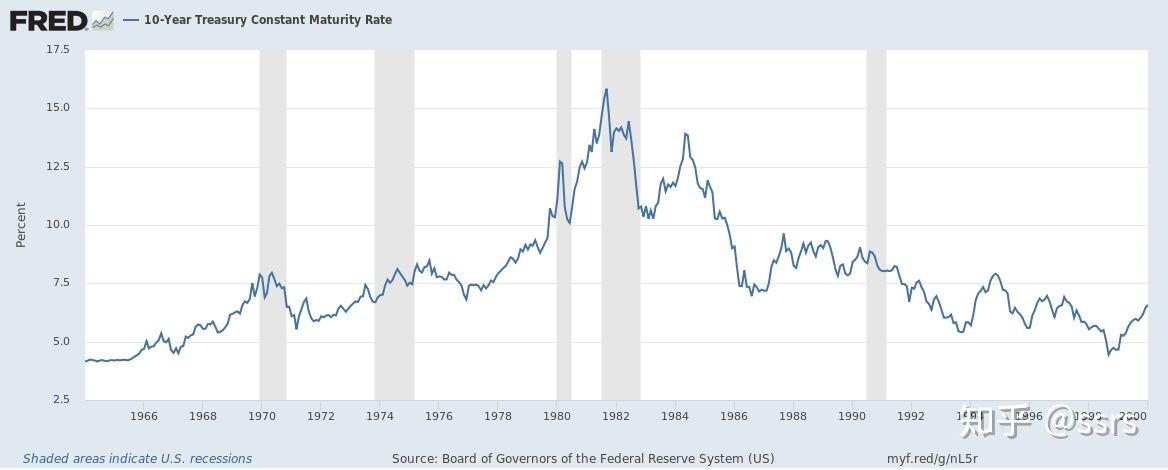
\includegraphics[scale=0.3]{lilv.jpg}
    \caption{十年期美国国债利率}
    \label{lilv} 
    \end{figure}

1964—1981年,美国长期国债的利率呈现大幅上扬的态势,从1964年年底的4\%飙升到1981年年末的15\%。这对各投资品的价格都造成了很不好的影响,其中最引人瞩目的便是股票价格,这间接解释了为何在这段经济腾飞的时期,道琼斯工业平均指数却原地踏步。另外一个原因是美国企业的利润,图51-1揭示了1929—1998年期间,美国企业税后利润占GDP的比重。从中可以看出,这个比重在1932年达到巅峰之后又大幅滑落,到了20世纪50年代开始在4\%~6.5\%间盘整,紧接着在1982年滑落到3.5\%的低点。因此,当时的股市投资者同时承受着两项负面因素的煎熬,利润大幅衰减,而无风险利率一飞冲天。投资者总会将目前所面临的状况投射到对未来的看法上,这好比是开车不看前方却紧盯着后视镜看,人们以为企业获利将持续低迷,无风险利率也会一直维持在高位,这再次解释了为何即使GDP已增长了近4倍而股市却还在原地踏步。

不过,在20世纪80年代早期,情况发生了大逆转。大家或许还记得保罗·沃尔克在就任美联储主席时有多么不受欢迎。然而,看看他之后的英雄事迹吧:在经济领域推行紧缩政策,抑制通货膨胀,这使利率走势产生大逆转,并带来了辉煌的硕果。假设你在1981年11月16日拿出100万美元购买30年期、票息率为14\%的美国国债,然后将利息进行再投资,即每次你拿到利息后,用这笔钱再去购买同样的债券。到了1998年年底,在长期国债的利率降为5\%的情况下,你的投资将增值至8181219美元,相当于你获得了超过13\%的复合年回报率。别小瞧这13\%的年回报率,它可比同时期内很多股票的表现抢眼多了,而且几乎胜过历史上任何一个17年的时间段。对于一只“貌不惊人”的国债来说,这样的回报可谓恢宏。

利率的下降对于股价的推升也有影响,当然,利率只是其中的一个因素,还有很多其他因素。我们来看看这17年内股市发生了什么:如果在这一期间,你以相同的100万美元投资道琼斯工业平均指数,到了1998年12月31日,你将会得到19720112美元,复合年回报率约为19\%。这在历史上是前所未有的成绩,甚至比在1932年股市大崩盘时的最低点购入股票(1932年7月8日,道琼斯工业平均指数收盘点数为41.22),然后持有17年还要好。

在这17年内,对股价产生影响的第二个因素就是企业的税后利润。下图向我们展示了企业的税后利润占GDP的比重的变化情况。通过这张图,我们能了解到,到了每年的年终,美国企业的股东们的所得究竟占GDP多大比重。
\begin{figure}[h!]
    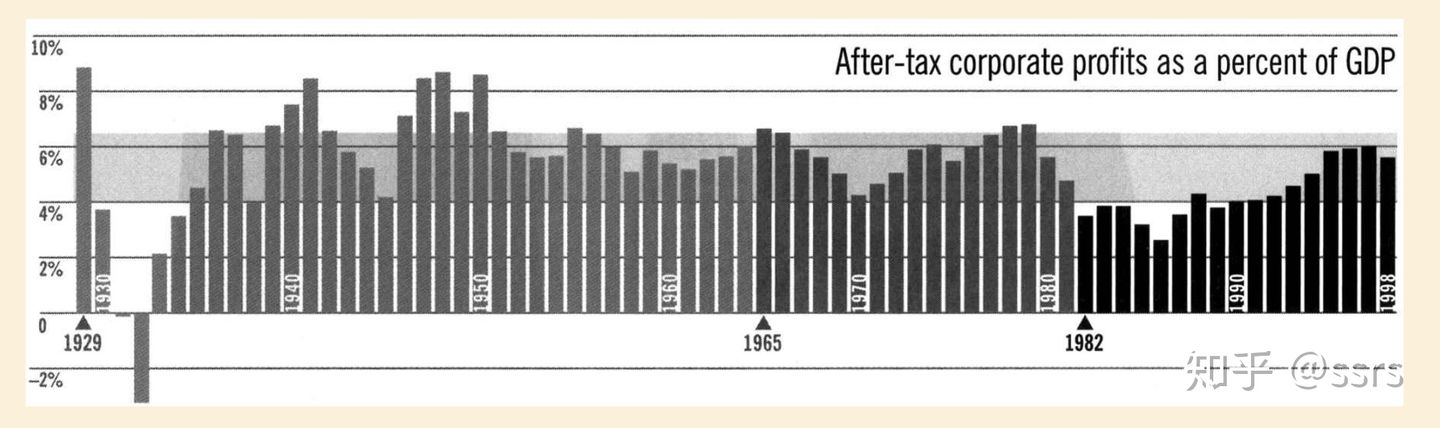
\includegraphics[scale=0.28]{gdp.jpg} 
    \caption{美国企业税后利润占GDP比重}
    \label{gdp}
\end{figure}

正如你们看到的,这张图 2 的起始年份是1929年。我个人非常喜欢这个年份,因为对于我来说,这是“一切”的起点。当时我父亲是一位股票销售员,在大崩盘到来之时,跟任何人打电话都会让他感到恐惧,因为电话那边的人的状况几乎都“惨不忍睹”。每天下午他就待在家里,当时还没有电视,所以……1929年11月30日前后,就有了我(9个月之后的1930年8月30日出生)。因此,大崩盘时常让我感到一种莫名的温暖。

正如你所看到的,在1929年,企业税后利润在GDP中的比重达到顶峰,然后就一蹶不振了。事实上,图表的左半边并不具有典型性:不仅包含了萧条期,还囊括了一段温和复苏的时期(这段时期受到超额利润税的制衡),以及战后另一段复苏期。从1951年起,该比重就开始固定了下来,一直保持在4\%~6.5\%的区间内。

然而,到了1981年,企业税后利润所占比重开始出现下滑的趋势,脱离了4\%~6.5\%这个区间。1982年时,该比重缩水到3.5\%。因此,当时投资者正面临着两种失衡的状况:利润低于预期,而利率又堪比天高。

很典型的现象是,投资者往往会把自己现在看到的景象投射到未来。这是他们根深蒂固的习惯:总是朝后视镜里看风景,而不是从前挡风玻璃中。所以,在展望未来的前景时,他们对国家的未来充满忧虑和沮丧。他们预计利率会继续走高,而利润会持续走低。因此,他们认为,道琼斯工业平均指数会回归到17年前的水平,即使GDP翻了接近两番。

那么,17年前的1982年究竟发生了什么呢?在第二个17年内,GDP方面没有发生可观的大幅提振。GDP的增长不足两倍,但是利率开始下调。沃尔克的“紧缩效应”逐步淡去之后,企业的税后利润率开始爬升,虽然还不太稳定,但无论如何,还是迈出了坚实的步伐。你可以从图51-1中看出税后利润的变化趋势,到了20世纪90年代后期,企业税后利润占GDP的比重已经接近6\%,也可以说回归到了“常态”时的较高水平。1998年年底,美国长期国债的利率降至5\%左右。

利率和企业税后利润,这两个投资者最在乎的要素的变化,虽然不是全部,但也部分解释了为何第二个17年美国股市的涨势超过10倍(道琼斯工业平均指数从875一路攀升到9181)。当然,大牛市也与市场心理因素有密切的关系。一旦牛市开始启动,人们会在某个时期发现,不管用什么方法都能赚大钱。因此,所有人蜂拥而至,不论利率如何,回报怎样,都不做考虑。他们认为,如果不投身股市,就会错失赚钱的良机,到时候追悔莫及。“我可不能错过这个大狂欢”的心理已经超越所有基本因素,成为主导市场的重要动因。大家早已变成俄国著名心理学家伊万·巴甫洛夫(Ivan Pavlov)实验下的那条狗,只要听到纽约证券交易所早上9:30的钟响就知道有东西可以吃。事实证明,他们的信心一天比一天强,甚至到最后还坚信,这一切都是老天爷所赐,是他老人家希望大家共同富裕。

此时通过回顾往昔,他们对未来更是充满了美好的期待。在1999年7月份,由佩因韦伯证券公司(PaineWebber)和盖洛普咨询公司(The Gallup Organization)公布的调查显示,投资经验不到5年的“菜鸟”投资者认为未来10年的复合年回报率竟高达22.6\%,而即使是有20年以上投资经验的“老鸟”,也认为应该是12.9\%。

现在,我要给大家泼一盆冷水,未来股市的复合年回报率可能连12.9\%的边都沾不上,我将通过梳理几个决定性因素来证明我说的话。如果投资者想在未来的10年、17年甚至20年获得丰厚的回报,我预计的三件事中至少将发生一件。三件事的最后一件我会在后面再谈,现在先说说前两条:

1、\textit{利率必定会继续下跌}。如果现阶段美国国债的利率为6\%,那么在将来会降到3\%左右,仅凭这一个因素,普通股的价格将会翻倍。如果你也这么认为或者认为国债的利率会降到1\%,就像日本曾经经历的那样,你就应该在会大赚一笔的债券期权上豪赌一把。

2、\textit{企业利润所占GDP的比重必定会大幅增长}。有人曾告诉我,纽约的律师比普通人还要多。我想这和某些人认为的利润率的增幅会比GDP增长率还高是一个道理。当你期待某个组成部分的增长率永远会领先于整体时,那你最好先去研究一下数学问题。在我看来,如果你相信企业利润占GDP的比重能够,而且,无论如何都会持续地超过6\%,那你一定是盲目乐观了。实际上,企业利润所占的比重是会下降的,而使其下降的一个原因就是竞争。现阶段,美国国内竞争很活跃,而且氛围很不错。除此之外,公共政策方面的因素也会导致企业利润率下降。如果投资企业的人一起分吃美国经济增长所带来的这块大蛋糕,而且胃口越来越大,其他团体不得不面对盘中越来越小的食物时,就会自然而然地产生政治问题。我认为,大规模地重新分配这块大蛋糕的局面只是还未发生。

那么,合理的推算又会带给我们什么结果呢?我们假设GDP的年增长率是5\%(实际年增长率为3\%),这已经是非常乐观的估计了,此外,还有2\%的通货膨胀。如果GDP的年增长率达到5\%,而利率又没什么变化,那么,股票的总体价格将不会上涨更多。当然,你还可假设股息率会高一点,但以目前的股价水准来看,股息所占的比重已大不如前,而通过大规模回购提高每股盈余的方法也没什么用,因为同时期也会有许多公司发行新股,一部分通过一级市场,另一部分通过股票期权。

因此,回到之前假设的5\%的GDP年增长率,我要提醒大家,你们未来的回报存在一个限制性条件:如果美国企业的利润增长顶多只能达到5\%,你就不能预期年投资回报率一直维持在12\%(当然远低于22\%)。实际上,不论何种资产,它的价格的增长速度不可能长期高于其利润的增长速度,这是不可逃避的现实。

或许你有不同的见解,想和我辩论一番,这也情有可原,那就把你的假设说给我听听。如果你觉得美国公众每年能够在股市上赚到12\%的回报,我想你就必须得这样回答:“那是因为我预期GDP的年增长率应该在10\%左右,回报上还要再加2\%的股息,而利率又保持在恒定的水平。”或者你通过其他的方式重新设置了这些关键变量。如果你相信的话,奇妙仙子小叮当的魔法或许帮得上你,你可以拍拍手,只不过得拼命拍,可别停下来。

此外,你还必须考虑到的一点是,未来的回报总是与当下股市估值水平有紧切的关系。让我们来看看现在投资美国股市到底能得到什么。以下是《财富》500强企业在1998年的两项重要数据。500强企业占据了美国股市总市值的75\%,所以,它相当于美国企业的缩影。

FORTUNE 500

1998 profits: \$334,335,000,000

Market value on March 15, 1999: \$9,907,233,000,000

当你仔细研究这两项数据时,必须注意的是利润部分“事有蹊跷”。1998年的利润中包括了一些非同寻常的部分。福特汽车公司计入了分拆旗下第一联合资本(Associates First Capital)所获得的160亿美元;另外总利润中还包括了很多互助公司的收益,比如国家农场保险公司(StateFarm Insurance Cos.),但该类公司没有参考的(公开)市值,这在《财富》500强企业中是常见的情况。此外,一项巨大的企业开销没有从利润中扣除,即股票期权的补偿成本。另一方面,一些不能反映经济现实的冲销,事实上是可以加回实际利润的。不过,抛开以上例外情形,按照1999年3月15日当日的行情来计算,美国股市的投资者等于每年花10万亿美元赚取了3,000多亿美元的回报。

要特别注意的是,本质上除了企业真正的利润,股票投资者作为一个整体不可能从股市中多赚一分钱。我们或许可以低买高卖赚取差价。然而,如果假设《财富》500强企业合并成一家企业,而所有投资者都拥有一小部分股权,那么这样一来,我们就如同坐在同一间房子里,相互之间买进卖出,将股价越炒越高。如果你比别人聪明,你确实可以逢低买入,逢高卖出,但事实上,你在游戏里拿走的钱都是另一个投资者投入的。与此同时,这种零和游戏对合并后的巨无霸“企业”的境遇并没有丝毫改变,因为它的命运完全取决于利润。无论是现在还是直至世界末日那一天,对于企业所有者来说,最重要的就是企业的实际利润,这是毫无疑问的。

还有另一个非常重要的问题值得考虑。如果你我只是在这间小房子里相互交易,我们就可以规避交易费用,因为这里没有经纪人来收取每笔交易的佣金。然而,在真实世界里,投资者总是喜欢换“座位”,或者至少咨询一下是否应该换“座位”,无论如何,这都会是一笔开销,而且是一笔很大的开销。他们承担的这笔费用(我把它称为交易费用)涵盖的内容相当广泛,比如做市商的差价、佣金、认购/申购产生的销售费用、12b-1费用、管理费、保管费和包装费,甚至还有订阅金融出版物的费用。千万别把这些开销当作无关痛痒的东西一笔抹去。如果你要投资一块房地产,难道在计算回报时你会将自己花费的评估费用忽略掉吗?当然不会。同样地,股票投资者在计算回报时,也必须扣除高昂的交易费用。

那么投资者到底为此花了多少钱呢?我的估测是:美国股票市场的投资者每年要支付超过1,000亿美元,准确一点是1,300亿美元,来改变自己的投资去向,或者向咨询机构购买建议。每年大约有1,000亿美元都花在了《财富》500强企业身上。换句话说,1998年,《财富》500强企业辛辛苦苦为投资者赚了3,340亿美元,投资者却拱手将其中的1/3送给了各种各样的咨询和“帮助”机构。在这之后,《财富》500强企业的股东们用他们10万亿美元的投资只获得了不到2,500亿美元的回报。在我看来,油水已经太少了。

或许你心里并不赞同,想和我辩论一下1,000亿美元是如何流向那些“帮手”的。我们来看看他们是如何收取费用的吧。先从传统的佣金说起,这其中包括手续费、做市商的抽成以及承销发行的差价。除去重复计算的部分,今年股市的交易量大约为3500亿股,如果按照每股每方(也就是买和卖都要支付)的佣金平均为6美分来计算的话,统计下来,这笔佣金也将达到420亿美元。

再看看其他开销:拥有包管账户的小户要面对巨额开支,大户则要支付管理费用,股票型共同基金的投资者还要支付一大笔骇人听闻的开销。这些基金目前拥有3.5万亿美元资产,而它们的投资者每年所要支付的各种费用,如管理费用、认购/申购产生的销售费用、12b-1费用以及运营成本等,总计至少将达到资产额的1\%,也就是350亿。

而且,以上我所提及的那些费用还未包括期权和期货的佣金和差价,或者是各种年费以及“帮手”们想出的层出不穷的各种费用。简而言之,《财富》500强企业的股东们无辜花掉了1000亿美元(相当于《财富》500强企业市场价值的1\%)。在我看来,这1000亿美元的费用不是说多了,而是非常保守的估计。

我觉得这是一笔可怕的开支。我曾听说过一部动画片,其中有一位新闻评论员说:“纽约证券交易所今天没有发生任何交易。每个人都满足于他们现在所拥有的。”好吧,如果这是事实,投资者每年就能为自己的口袋保住1300亿美元。

关于股市,我来总结一下自己的观点。我认为,实在很难找到一个具有说服力的证据来证明,在接下来的17年里,股市的回报率将会像它过去17年中的表现一样好。如果让我预测一个最有可能的回报率数字,包括增值和股息,在利率稳定、2\%的通货膨胀率和居高不下的交易费用的基础上,投资者最后整体可能得到的结果是6\%,我要强调一下,是整体。如果在这个基础上再刨除通货膨胀率(不论通货膨胀率涨跌情况如何,都要刨除这个部分),那就是4\%。如果4\%字有误,我相信正确的数字只可能更低。

回到我早先说过的话题上:投资者若想在未来的股市上获得丰厚的回报,有三件事不可或缺。第一,利率继续下跌;第二,企业利润所占GDP的比重大幅提升。现在我来谈谈第三点。或许你是一位乐观主义者并坚定地认为,尽管从整体上来说,股市投资者前景堪忧,但你自己总能成为股市中的佼佼者。在信息革命(我个人无比膜拜的时代)的初期,这种想法听起来颇具诱惑力。你的经纪人或许会告诉你,选择那些明显的大牛股,把握这波超级趋势!

回顾一下20世纪前半段改变我们生活的那些工业,比如汽车制造业和航空业,应该会对我们大有裨益。先来谈谈汽车制造业,美国汽车与卡车制造业者的名单能写满70页纸。其中两家制造商的名字很自然地引起我的注意,一家名叫伯克希尔,另一家叫奥马哈,当然还有许多其他汽车制造商。

正如你所听到的,汽车制造业是一个拥有超过2000家制造商的庞大工业,对人们的生活有着难以估量的影响。如果在当时你具有足够的见识,就一定会说“这是一条通往富裕的道路”。然而,情况发展到20世纪90年代又如何呢?这些公司经过多年的竞争厮杀之后,只剩下三家,这对投资者来说全然不是好事。因此,可以这样说,这是一个对美国影响深远的产业,但对投资者的影响未必是那般辉煌。

在汽车制造业的蓬勃发展这种革命性的事件中,有时我们反而比较容易断定输家。人们很容易体会到汽车产业的重要性,却很难挑选出能为自己赚钱的企业。如果时光可以倒流,我相信你就可能会做出这样一个决定:有时候把事情颠倒过来看可能更好,做空那些受负面影响最大的事物,比如马匹。坦白地说,我很惋惜为何巴菲特家族当初没有做空马匹。而且这实在很难说得过去:住在内布拉斯加州,本可以很容易借到马匹以避免被别人“逼空”。

U.S. Horse Population

1900: 21 million

1998: 5 million

除了汽车产业之外,20世纪另外一个革命性产业就是航空业,这是一个让投资者想到美好未来便口水直流的新兴产业。我特地查阅了当初所有飞机制造商的资料,发现在1919—1939年,大约有300多家公司,但现今可能只剩下几家还在苟延残喘。当时生产的众多飞机中有两架名叫“内布拉斯加”和“奥马哈”号的飞机,现在即便是最忠诚的内布拉斯加人恐怕也不敢驾驶这样的飞机驶向蓝天吧。

接下来,我们来看看航空业是如何走向衰落的。最近20年宣告破产的航空公司有129家。自从航空业陷入不景气以来,所有航空公司加起来的净利润是零,也就是说连一毛钱也没赚过。我在想,如果当初莱特兄弟的小鹰号第一次起飞时,我在现场,我很可能会极具远见地、充满公益心地(这点是为了未来的资本家)设法将它打下来。

我的意思是,莱特兄弟对于其他深深地改变了美国人生活方式,但对投资者没什么好处的辉煌产业,比如收音机与电视等,我不再赘述。不过我从中得出这样一个结论:\textit{投资的要旨不在于评估这个产业对社会能有多大的影响,或是它有多大的发展空间,而主要应该看某家公司有多大的竞争优势,还有更为重要的一点是,这种优势能维持多久。拥有广阔而持久的“护城河”的产品或服务才能真正为投资者带来甜美的果实}。

17年这样一个时间跨度不禁使我联想到17岁的“蝗虫”,虽然这么说有点儿突兀。这些计划飞进2016年的小生命,到时候又会有怎样的际遇呢?到那时对于股票的看法或许更冷静、理智,不像现在这般欢欣雀跃。自然,投资者对此可能会感到失望,不过,这只因为他们开始时期望得太多。

无论如何,他们那时一定比现在富裕得多,原因很简单,因为他们所拥有的美国企业将会继续发展,而且其利润以每年约3\%的速度增长。最值得我们高兴的是,新生的财富将最终惠及美国大众,美国人整体的生活水平将比现在更上一个台阶。即便未来达不到在过去17年美国投资者业已习惯的那种大跨步式的发展,也注定不会是一个糟糕的世界。

\section{股东手册}

在1996年6月,伯克希尔董事会主席沃伦·巴菲特向公司A股和B股的股东分发了一本名叫“股东手册”的小册子。其目的是解释伯克希尔主要的营运经济原则,以下是这本小册子的升级版本。
\subsection{与股东相关的商业原则}

在1983年合并印花蓝筹公司(Blue Chip)的时候,我立下了13条与股东密切相关的商业原则,希望这将协助新股东理解我们的管理方式。正如“原则”的涵义,13条则完整保留至今,在此以楷体列出。
\begin{itemize}
    \item [1.]
    \textit{虽然我们的形态是企业但我们的态度却是合伙事业。查理·芒格和我都将我们的股东视为经营合伙人,而我们自己则为经营伙伴 (由于持有的股权规模之故,姑且不论好坏,我们也是控制伙伴)。我们并未将公司视为所拥有事业资产的最终持有人,反而是将其视为我们股东拥有资产的一个管道。}
    
    查理跟我希望你们不要认为自己只是拥有一张价格会每天波动的纸张,而这张纸只是当某些使你紧张万分的经济或政治事件出现,你选择抛售与否的选项之一。我们反倒希望你将自己视为是某个事业的部分所有人,而这事业是你愿意永久保留的,如同你可能跟其他家庭成员共同拥有一座农场或是一间公寓一般。对我们而言,我们不会将伯克希尔的股东视为一群常变动的无名氏,而是愿意将他们原本可以用以安度余生的资金托付给我们一同参与冒险的伙伴。
    
    证据显示大部分的伯克希尔股东的确欣然接受这长期伙伴的概念。伯克希尔股票每年的周转率相对其他大多数美国企业来说只是很小的比率,即便是把我所持有的股份排除在外来计算亦是如此。
    
    实际上,我们的股东对伯克希尔股票的影响与伯克希尔对其投资的影响如出一辙。就好比伯克希尔亦是可口可乐或美国运通的股票持有人,我们视伯克希尔为这两家卓越公司的不具管理权限的伙伴,而我们以公司长期发展的成果来衡量我们的绩效而非每月股价的波动程度。事实上,就算这些公司在市场上长达数年都没有交易或是报价,我们也完全不在意。如果我们抱持长期的展望,短期股价的变化对我们来说是无任何意义的,除非是他们出现提供我们增加其持股机会的诱人价格。

    \item [2.]
    \textit{为了与伯克希尔股东导向一致,我们大部份的董事都将其大部分净资产净值投资在公司上,我们可是自食其力。}

    查理的家族大量资产净值形式是持有伯克希尔的持股;我个人则是 98\%。除此之外,我很多亲属例如,我的姊妹以及堂或表兄弟姊妹他们资产净值中也都有很大比例是伯克希尔的持股。
    
    查理跟我对于这种把鸡蛋放在同一个篮子的情况感到放心,因为伯克希尔本身拥有各式各样真正优异的企业。的确,我们深信伯克希尔拥有的股权无论具控制权与否,已经是近乎唯一在质与多样性上兼具的公司。
    
    查理跟我无法承诺你结果将会是如何。但是我们可以保证不论你是在哪个时期决定成为我们的合伙人,你的财富将与我们的财富一起成长。我们对于巨额薪酬、期权或是其他赚取超过你的好处没兴趣。我们只跟我们的合伙人赚同比例的钱。此外,当我做了某项蠢事,我愿你能从我也将蒙受同比例的损失这件事上得到一些慰藉。

    \item [3.]
    \textit{我们长期的经济目标(容我在稍后再对此作描述)是以每股内在事业价值为基础追求伯克希尔最大的年化报酬率。我们不用伯克希尔的公司规模来衡量其经济重要性或绩效;我们通过每股进程来决定。我们可以确定在未来巨幅扩张资本的基础下将见到每股表现每况愈下。但若是我们的成长率没有超越美国大型企业的平均水准我们将感到失望。}

    \item [4.]
    \textit{我们偏好通过直接拥有多种可产生现金且资本报酬恒常高于一般水准的事业群来达到我们的目标。我们次佳的选项则是通过我们旗下保险子公司在公开市场买进普通股进而拥有上述特质企业的部份股权。价格、可行性以及对保险资本的需求状况决定我们在特定年期中的资产配置方式。}

    近几年我们已经完成几项并购。即便必定出现荒年,我们依旧期待后续数十年完成更多更大项目的并购案。若是这些收购接近我们过去所达到的品质,伯克希尔将得到更好的成果。
    
    对我们最大的挑战在于我们孕育新构想的速度必须跟我们产生现金的速度一样快。基于这个因素,一个萎靡不振的股市比较可能让我们发挥显著的优势。首先这样可以降低所有企业的价格使其更可被收购。其次一个低迷的市场让我们的保险公司得以用吸引人的价格买下卓越公司的部份股权(包括我们已经持有的公司也可增加其持股)。第三点,有些优异的公司持续回购自家的股份,这意味他们跟我们都可以从买进较便宜的股票这件事上得到益处。
    
    整体说来,伯克希尔及其长期持有人都可以从下跌的股市中得到好处,正如同一般食物采购人可以从食物价格下跌中得到利益一般。所以当股市总是一次又一次发生崩跌时,无需恐慌或是哭丧着脸,要知道这对伯克希尔来说可是天大的好消息。

    \item [5.]
    \textit{由于我们对于事业所有权采两手策略的态度并受限会计的先天限制,合并报表所载的盈余数字可能仅揭露我们实际绩效的一小部分而已。查理跟我既身为公司的拥有人也是经理人,我们实际上会忽略这类合并数字。然而我们也会向你报告每个我们实质控制事业的盈余,这才是我们认为最具重要性的数字。这些数字会在我们提供个别事业的信息中一并出现,相信对于你在判断他们的表现上会有帮助。}

    为了让事情简单化,我们试着在年报中呈现给你真正重要的数字跟信息。查理跟我付出大半心力在关注我们的事业表现如何以及各事业所处产业环境的运作情形。举例来说,我们的事业体究竟是在搭产业循环的顺风车或是被该产业大环境不佳拖下水?查理跟我需要确切知道目前的情况并借此调整我们的预期。我们也会把我们的结论传达给你知悉。
    
    长久以来,我们大部分的事业体都有超出我们预期的好表现。但有时也有令我们失望的情况发生,我们将尽可能坦率地向你告知这类信息一如我们过去在描述较愉快的经验那般。当我们用非传统的方法去评估我们的进程(例如你在我们的年报中所读到的保险「浮存金」),我们将试着解释这些概念以及为何我们重视他们的原因。换句话说,我们深信在告知你我们的想法后,你不但能评估伯克希尔旗下的事业体,也能将其运用在管理及资产配置上。 

    \item [6.]
    \textit{会计上的结果并不影响我们的营运方针或资产配置决策。当并购成本相近,我们倾向购买在标准会计准则认定报告台面下具有 2美元盈余的标的,而非台面上仅有 1美元盈余者。这正是我们经常在收购一完整事业体(其盈余为台面上的算法)的一小部分(其盈余大部分是在台面下的)时会做出支付相当于一般估算两倍价格决定的原因。总之在经年累月之后,我们期望这些台面下盈余最终将透过资本利得反映在我们事业的内在价值。 }

    我们发现经过一段时日后我们投资部位的未分配盈余对伯克希尔的取向与这些盈余直接分派给伯克希尔相当(也因此都会被覆盖在我们官方报告的盈余中)。这个令人高兴的结果会出现是因为我们的投资对象都处在真正卓越的业务中,他们总能运用额外的资本获取更大的利益,不管是将资本投入自己的业务中还是回购自己的股票。显而易见,我们投资对象的所做的每个资本决定没有让我们这些股东获益,但整体说来,他们每保留一美元盈余,我们就能得到中得到远远超过一美元的好处。我们因此将实质盈余考虑到我们营运年度收益的最佳写照。

    \item [7.]
    \textit{我们很谨慎地利用融资,并且当我们真的得借贷时,我们总试图以长期固定利率的型态组织我们的补偿。 这样的保守原则对我们并非有利,但顾虑到我们对于被保险人,放款人以及很多将自己大半毕生心血交付给我们的股票持有人 (诚如一位印第安纳波利斯的“ 500”获胜者的玩家所言:想要完成比赛获得第一名,首先得先完成比赛) }

    查理跟我所运用的财务计算,绝对不会牺牲我们一夜好眠只为了换取一丁点额外的报偿。我相信不须要为了追求我的亲友们没有或不需要的东西,而让他们涉足不必要的风险。
    
    此外,伯克希尔已拥有两种低成本且无风险的举债来源:递延所得税及「浮存金」(我们拥有的保险事业所持有的另一种资金,主要是从我们收取保费后到需要赔付这段期间所衍生),这允许我们可以更安全拥有远超过单靠我们资产净值所能持有限制的总资产。这两种资金来源快速成长至今已达到总共 1700 亿美金的规模。

    更棒的是,这些资金到目前为止还经常是零成本的。递延所得税负债项目不需要利息,而且只要我们能打平再保的成本,营运产生的浮存金的成本一样是零。当然啦,这两者都是真的负债而非资产净值,但他们是没有附加条款或是到期日的负债。实际上,这两者给我们债务的好处(有能力拥有更多资产来为我们工作)却没让我们承受一般债务所具缺点的重担。

    当然,并没有人可以保证未来我们还是可以获取零成本的浮存金。但我们感觉我们跟其他保险同业有相同机会达到这个目标。不仅我们在过去达到这目标(排除你们的董事长所犯下的一些重大过失),我们在 1996 年并购 GEICO 后,大大增进我们取得零成本浮存金的可能性。

    在我们当前的配置里,我们想更多的借款-那些对伯克希尔没有追索权的借贷,集中用于我们的公用事业及铁路业务上。此时,我们偏爱长期固定利率的贷款

    \item [8.]
    \textit{管理阶层的「希望清单」将不会让股东埋单。我们不会只为了多样化经营而用控制价格去购买整个企业,却忽视股东的长期经济利益。我们只会用你的钱去做我们用自己的钱会去做的事,就像你会权衡自己能透过多样化自己的投资组合可获取多少价值后才经由股市购买股票一般。}
    
    查理跟我只有在确信我们可以提高伯克希尔股票的每股内在价值之后才对该并购案感兴趣。我们的酬劳多寡或是办公室大小都跟伯克希尔资产负债表的规模无关。

    \item [9.]
    \textit{我们觉得崇高的目标应该经常以成果来检验。我们透过评估每保留一美金盈余经过一段时间后,股东们是否可从市值得到超过一美元效益,来检测我们对保留盈余的看法是否正确。至今为止,这样的检验始终与我们的看法一致。我们将持续用往前回溯五年的基础来运用这方式。随着我们的资产净值成长,要明智地运用保留盈余将渐行困难。}

    我应该把“五年滚动基础”这句话另外表述的,直到2009年股东大会上我碰到一个关于这方面的提问时,我才意识到自己犯了个错误。
    
    当股票市场经过一个5年的行程大幅下跌后,我们的账面价值对应的市场价格有时会收缩。当这个情况出现时,我们没有通过检验因为我没有正确的表述它。早在1971到1975年,就在1983年我写下这些原则前,我们就落后很多。
    
    五年检验必需满足以下条件:(1)在5年中,我们的每股收益确实超越了标普指数的表现;(2)我们的股票持续的以超过账面价值的价格交易,意味着每保留的1美元收入市价都超过了1美元。如果这些条件达到了,保留收入才有意义。

    \item [10.]
    \textit{我们只有在当我们能付出跟获取等量事业价值时才发行普通股。这规则适用于所有发行型态(不只是并购或公开发行,还包括股债转换、股票选择权以及可转换有价证券)。在与整个企业价值不一致的前提下,我们将不会出售你的公司的一小部分(亦即总发行股数的对应数量)。}

    当我们于 1996 年售出 B 股时,部分投资人对我们指称伯克希尔股票的价值并未被低估感到震惊。这样的反应实在是毫无根据。他们应该感到震惊的反而是我们当初登记发行的股票被低估这件事才对。当公司的高层在公开发行期间明说或暗指他们的股票价值被低估时,通常时依据的是公司当时实际经济情况,而非依照原股东的持有成本而言:因为假如他们的经理人刻意用80美分的价格出售实际价值1美元的资产,将对股东造成不公平的损失之前我们在发行B 股时不曾犯过这样的罪行,往后也绝对不会。 (然而,我们在当时并未宣称我们的股价被高估,许多媒体却都报导我们确实有这么做)。

    \item [11.]
    \textit{你必须确实了解到查理跟我所分享的一种并不利于我们的财务表现态度:不管股价为何,我们毫无兴趣出售伯克希尔旗下所拥有的优秀企业。只要我们预期他们至少会产出些许现金,并且只要我们对其劳资关系感到满意,我们也非常不情愿出售表现低于平均水准的事业体。我们只希望入主次级事业体这种资产配置的错误不再重复发生。我们将对那些声称只要对我们旗下表现不佳的事业体大幅提高资本支出即可让公司回复到令人满意收益的建议严正警告(这些推论看似前途似锦而且倡导人往往态度诚恳,但到了最后,对一个糟糕透顶的产业大量额外的投资通常得到的只是像陷入流沙般那样苦苦挣扎)。尽管如此,唯利是图的管理行为(每次都抛弃你认为最不具前景的事业体)并非我们的风格。我们宁愿为保有全部成果而受点责罚,也不愿意干出那种勾当。}

    我们持续避免出现唯利是图的行为。的确,我们在苦撑 20 年后最终仍在 1980 年代中期关闭我们的纺织事业,但这只因我们认为它已经陷入无穷无尽的营运亏损深渊之故。不过我们既不会以高价出售某些业务也不会摒弃我们表现较差的部分,我们会聚焦在解决造成它们表现不佳的原因。为了澄清在2016年出现的一些质疑的声音,我们强调此处指的是我们控股的业务,而不是可交易的股票。 

    \item [12.]
    \textit{我们将直言不讳地向你报告,并在评估企业价值时强调对其造成增减的重要项目。我们的指导手册主要是告诉你那些即便我们彼此的立场互换,我们也会想知道的各事业体的实际营运状况。我们绝对不会亏欠你。此外,就像一家传播公司在资料正确性上对我们大打折扣是非常不可原谅一般,我们会对自家公司有更平衡及深入的报告内容,如同我们要求自己的新闻从业人员报导别人一般。我们同样相信真诚对管理阶层的好处会跟我们一样:公开误导其他人的 CEO 最终也会自欺欺人。}

    在伯克希尔你找不到会计花招或重组的"洗大澡"行为,也不会发现任何对季报或年报结果做任何的美化。我们总会告诉你我们在每一洞击出多少竿且绝不会在计分卡上玩任何花样。当保险准备金需要被粗略概估时,我们将试着沿用我们那套前后一致且保守的方式来施行。

    我们会用几种方式跟你联系。通过年度报告我试图给所有股东在合理的文件篇幅中尽可能多的价值定义资讯。我们也会试着在发布到网路上的季报中呈献给你充足却扼要的重要资讯,虽然这些并非出自我手(个人秀一年一次就够了)。另一个重要的联系场合正是我们的年度聚会,在这里查理跟我很乐意花五个小时甚至更多时间去回答各位有关伯克希尔的种种问题。但是有种交流的方式我们则无法提供:一对一的交谈方式。这对于拥有成千上万股东的伯克希尔来说实在窒碍难行。
    
    在我们所有的联络方式中,我们试着确保没有任何一个股东拥有优势:我们不会遵循给财务预测的常规或是将其他有价值的资讯透露给分析师或大股东。我们的目标是让所有股东在同一时间得到第一手信息。

    \item [13.]
    \textit{尽管我们有坦白这项行事方针,我们只会在法律要求的前提下,讨论我们对于上市有价证券的买卖情形。绝妙的投资点子是很稀有而且珍贵的,且如同好产品或优秀企业并购案那般极易遭致竞争对手的觊觎。所以我们通常不讨论我们的投资想法。这个禁令同样适用于我们已经出售的股票(因为我们可能会再买回)以及谣传说我们将买进的标的。如果我们否认所有报告内容但却在其他场合表明「不予置评」,那么这个不予评论就应该是确认了。}
    
    虽然我们仍然没有意愿对特定股票表达看法,我们却可对我们的事业及投资哲学畅所欲言。我个人从睿智慷慨且堪称金融史上最伟大的导师——本·格雷厄姆身上获益良多,即使本的教诲也调教出其他伯克希尔新的投资对手,而我依旧深信从他学习到的隽永智慧亦将助我继续前行。
\end{itemize}
\subsection{两条新增原则}
\begin{itemize}
    \item [14.]
    \textit{在尽可能的情况下,我们希望每位伯克希尔的股东在他们持有股票的期间,可以通过同一时期公司每股的内在价值增减幅度等比例的反应在市价的增减纪录上。这么一来,伯克希尔的内在价值就必须和其市值的比例呈现一个定值,而我们倾向让两者是一比一的关系。如前所述,我们宁愿看到伯克希尔的股价维持在公平的水准而非较高水准。很显然地,查理跟我不会控制伯克希尔的股价。但是透过我们各种的行事方针及沟通渠道,我们可以轮流鼓励消息灵通且行为理性的投资人间接让伯克希尔的股价趋于合理。我们「高低估一样糟糕」的作法可能会让某些投资人感到失望。然而,我们相信这样的方式才是最有可能使伯克希尔吸引那些愿意陪伴公司成长,而非是只想藉由其他投资人犯的过错寻求利益的长期投资人。 }
    \item [15.]
    \textit{我们经常拿伯克希尔每股帐面价值的增益与 标普 500指数的表现相比较。长此以往,我们希望能超越这个指标。要不然,为什么我们的投资人还需要我们呢?然而这样的检验方式有个特定的缺点,我将在下个章节描述这个缺点。此外,目前这样的年增率比较方式已经比过去来得没意义多了。此乃肇因于我们目前净值中持有的股票其价值仅有一小部份与 标普500 连动,这与早年的情况截然不同。除此之外,标普500指数 股票收益乃全由其指数计算而得,而伯克希尔持股由于联邦税制的关系只有 79\% 能计入。所以我们期望在股市了无生气的年度里胜过 标普500指数,而在股市过热表现的几年表现不佳我们倒不介意。}
\end{itemize}

\subsection{内在价值}
现在让我们把焦点放在我先前提到且将来你在年报中会遇到的一个名词。内在价值是个能提供唯一具逻辑估算各投资项目或事业体的相对吸引力的一个极重要概念。内在价值可以被简单定义为:一个事业在其存续期间所有产出现金的折现值总合。

虽然内在价值的估算并不容易。如我们所提出的定义,内在价值乃是一个估计值而非一个确切的数字,而且随着利率的变化或是对于未来现金流量的预估被修正,都需要对其重新估算。此外,就算两个人看到一样多的事实依据(这同样适用在查理跟我的身上),仍然不可避免出现些微差距的内在价值估算结果。这也是从未给你我们对于内在价值估算值的主要原因之一。虽然在我们年度报告中提供的诸多事实正是我们自己用以计算内在价值的基础。

同时,我们定期报告我们每股的帐面价值,虽然这是个容易计算的数据,但实际能运用的情况却有极其有限。这些限制并非从我们持有的那些上市有价证券中产生(其市值持续反映在我们帐上)。而是帐面价值不足以彰显我们掌控的公司,其帐面上所载净值可能完全迥异于内在价值。

情况也可能完全相反。举例来说,在 1964 年我们确信伯克希尔每股帐面价值为 19.46 美元。然而这数字有些夸大了公司的内在价值,因为所有公司的资源几乎与无利可图的纺织事业牢牢绑在一起。我们的纺织事业相关资产所登载的帐面价值,既与其继续营运的价值不符,也与其清算价值不相当。然而今日伯克希尔的情况刚好相反:目前我们的帐面价值远低于伯克希尔的内在价值,主要原因在于我们所控管的很多事业体其内在价值比他们所登载的帐面价值高得多了。

即使上述的说明显示帐面价值有不足之处,我们依旧给你伯克希尔的帐面价值等数字,因为如今这些数字提供一个尽管有些粗略、不充分但却不失为追踪伯克希尔内在价值的一个方式。换句话说,任何年度帐面价值变化的百分比很可能适度地接近其内在价值的年度波动程度。

通过观察大学教育这一种投资可以帮助你对于帐面价值跟内在价值之间的差异有更深刻的了解。我们先将教育成本视为他的「帐面价值」。假如这成本要是个很精确的数字,那么应该将该名学生选择求学而放弃工作所可能获取的收入列入考虑。

在这个练习中,我们将忽略教育在非经济性的重要效益并且只聚焦在其经济价值上。首先,我们必须推估该名大学毕业生往后人生可赚取的收入,并扣除他若未受该项教育其工作所得的估计值。这给我们一个额外的获利数字,接着将该数字以一个合适的利率折现,并回推到其毕业典礼当天。求得的结果相当于该教育的内在经济价值。

有些大学毕业生将发现他们所受教育的帐面价值超过其内在价值,这表示无论是谁受该教育都是花冤枉钱。在其他情况,一项教育投资的内在价值将远超过其帐面价值,而这结果证明资本被明智地分配。很显然在所有情形下,帐面价值都是内在价值一个毫无意义的指标。

\subsection{伯克希尔的管理}

我认为通过讨论伯克希尔今后的管理来作此篇总结应该是挺恰当的。如同我们股东相关守则第一条所述,查理跟我是伯克希尔的管理搭档。但我们把管理事业群比较吃重的工作都交由子公司的经理人代劳。事实上,我们几乎委派所有工作给其他人并退居幕后:虽然伯克希尔拥有 377,000 个员工,其中却只有 26 位在总部服务。

查理跟我主要参与资产配置以及我们重要经理人的培植。这些经理人在他们独挑大梁时最感到愉快,而这正是我们对待他们的方式。这样的安排让他们得以全权负责营运决策并且得以上缴多余的资金给总部。而将多余资金交付给我们可以让他们不会为了要配置资金到他们个别事业上而遭遇各种用度金钱伴随的诱惑而分神。甚且,查理跟我在投资运用这些资金上本来就比我们谨守自己领域的经理人浸淫在更大范围的机会之中。

我们大部分的经理人本身都很富有,所以我们有责任创造一个可以鼓励他们为伯克希尔工作的良好氛围而不是花时间在打高尔夫球或钓鱼上。这使我们必须公平地且设身处地以我们自己也愿遵守的规范来对待他们。

提到资产配置,这可是一个查理跟我都很乐在其中且获得不少宝贵经验的活动。一般认知上,即便头发花白,在这个领域也不会受到任何影响:你不需要好的手眼协调能力或是健硕的肌肉就可以灵活调度资金(谢天谢地)。只要我们的心智精明依旧,查理跟我就能像从前一样做好我们分内的工作。

在我死后,巴菲特家族将不会介入事业的管理,而只会当个坚实的股东协助遴选并监督经理人。当然,这些经理人何时上任得视我何时过世来决定,但是我可以事先决定管理架构:基本上我的工作将会分成两部分。一个高层主管将会成为 CEO负责所有营运。投资相关的重担则会落在一个或多个高阶主管的身上。假如有一个新的合并案已经开始进行磋商,这些高阶主管将会协同做出决策,当然啦,最后还是必须提交董事会同意才行。我们将会继续保有一个关注股东权益的卓越董事会,其相关利益绝对会与你一致。

一旦我们急切需要如我前述的管理架构,我们的董事们知道我对这两项职务的建议人选。所有候选人目前不是正为伯克希尔工作就是随时都可以走马上任,他们都是我可以完全信任的人选。

在继任人选这个议题上,我将继续保有董事资格。在我死后相当长的一段期间,我全部的遗产都会由伯克希尔股票组成,且这些股票将化为各基金会等价的资产,所以你可以确信董事们跟我对于继任人选的问题必有通盘的考量并早已为此做好万全准备。你同样可以确定的是我们经营伯克希尔至今所运用的各项准则亦将持续带领那些继承我遗志的经理人,而我们非凡坚韧且定义明确的企业文化将原封不动地持续下去。

唯恐我们以哀戚作结,我要你知道我过去从未感到像现在这样活力充沛,所以你大可放一百个心。我爱极了参与伯克希尔的运作,此外若享受生命有助于延年益寿,麦修撒拉(译注:圣经记载非常高寿的人)的纪录就岌岌可危了。 
\section[伯克希尔:过去、现在、未来]{伯克希尔:过去、现在、未来\footnote{原文刊登于2014年致股东信后附件。}}
\subsection{一切的开始}

1964年5月6日,伯克希尔·哈撒韦,当时是由一个叫做Seabury Stanton的人经营。他送了一封信给股东,打算用 11.375 元每股的价格,从股东手中,买 225,000股。我期待着这个信件,但却惊讶于这个价格。

伯克希尔当时拥有 1,583,680 股的外在股本。巴菲特合伙人企业,即我管理的投资实体,并实际上是我的净资产的企业,大约拥有其 7\% 的股份。在那个出价寄给我前不久, Stanton 询问我,要让我的企业出售所持股份,要给出什么价格。我回答说 11.50 元.他说:“好,成交。”而后,伯克希尔的信件来了,价格少了 0.125 元(即还是 11.375)。我对 Stanton的行为感到愤怒,所以没有响应。

这是个巨大的愚蠢决定。

伯克希尔当时是一个北方的纺织品制造企业,处于困境之中。这个行业正在向南方转移,不论是隐喻的,还是物理上的。伯克希尔呢,因为多方面的原因,不能相应做出改变。

行业的问题,长期以来都被广泛地理解。伯克希尔自身的董事会会议记录,1954 年 7月 29 日,记录下了惨淡的事实:“新英格兰地区的纺织行业在 40 年前就开始停业。在战争期间,这个趋势停止了。然而,这个趋势一定会继续,直到供给需求处于平衡为止。”

大约是董事会议一年后,两家 19 世纪就成立的公司,伯克希尔公司和哈撒韦公司,走到了一起,用了我们现在采用的名字。拥有 14 个工厂和 10,000 名员工,合并后的公司变成新英格兰地区的纺织巨头。然而,两家公司视为合并协议的文书,很快变成了自杀的契约。在合并后的七年间,伯克希尔的经营整体上是亏损的,净值减少了 37%。

与此同时,公司关闭了九个工厂,有时候用清偿的收入去回购股票,这个模式,引起了我的关注。

1962 年 12 月,我用巴菲特合伙人企业,第一次购买了伯克希尔股票,预计更多的关闭工厂和回购行为。那时候,股价是 7.5 美元,相比于运营资本 10.25 元和账面价值 20.20元,是大幅度折的。在这个价格买他家的股票,就像是捡让人抛弃的烟蒂,还可以再吸一口。尽管烟蒂可能难看或者乏味,吸的那口却是免费的。然而,一旦享受了短暂的愉悦,就再也没有什么能够被期待的了。

伯克希尔随后如预想的那样:它很快地关闭了其他 2 个工厂,在 1964 年的运动中,它开始用关闭公司的收入来回购股票。Stanton 那时候给的报价,是我们原始买入成本的 50%以上。它们,我免费吸烟蒂的机会,正在等着我呢,在吸几口后,我可以去别处寻找那些被抛弃的烟蒂。

相反地,愤怒于 Stanton 的欺骗,我忽视了他的回购报价,并开始大量地买入更多的伯克希尔的股票。

到 1965 年 4 月,巴菲特合伙人企业拥有 392,633 股(当时有 1,017,547 股外发股本),并且在 5 月上旬的董事会上,我们正式地控制了公司。通过 Seabury 和我的孩子气的行为——毕竟,1/8 美元,对于我或者他而言,算得了什么?——他丢掉了他的工作,而我发现我自己用了多于 25%的巴菲特合伙人企业的资本,投资在一个糟糕的生意,而且我对此生意知之甚少。我变成了那只追逐汽车的小狗。

因为伯克希尔的运营损失和股票回购,它的净资产,在 1964 年的财务年度末期,从 1955年合并的 5500 万美元的高峰,降到了 2200 万美元。2200 万美元全部都用在了纺织方面的运营上,公司没有多余的现金,并且倒欠银行 250 万美元(伯克希尔 1964 年年报,在本年报的 130-142 页重新印制)。

有段时间我很幸运:伯克希尔很快就享受了两年的好的运营状况。更好的是,它在那几年的收入是不需要缴交收入税收的,因为它拥有大量的延后亏损,源于前几年的灾难后果。

很快蜜月结束。在 1966 年之后的 18 年时间里,我们在纺织行业,经历了持续不断的挣扎,却全无效果。但是倔强——愚蠢?——是有限度的。在 1985 年,我终于认输了,关闭了运营。

我第一个错误,即把巴菲特合伙人的资源投入到将死的生意中,并未阻止我继续犯错,我快速地恶化错误。事实上,我的第二个错误,要远远比第一个严重,最终是我职业生涯中最昂贵的一个。

早在 1967 年,我让伯克希尔支付 860 万美元去购买国民保险公司 NICO,一个小型的,但有前途的奥马哈的保险公司(一个小的姐妹公司同样包括在这笔交易中)保险行业是在我的舒适区的:我理解并喜欢这个行业。

Jack Ringwalt,NICO 的拥有者,是我的长期朋友,他想把公司卖给我——我个人。他的报价,决不是给伯克希尔这个公司的。所以,为什么我为伯克希尔购买 NICO,而不是为巴菲特合伙人企业呢?我有 48 年时间去想这个问题,始终没想到好的答案。我只是犯了一个大错误。

如果巴菲特合伙人是购买者,我的伙伴和我,将会拥有一个 100%的好生意,注定会形成构造现今伯克希尔这样的基础。此外,我们的成长,将不会受到将近二十年时间的,困于纺织运营中的无效资本的妨碍。最后,我们接下来的并购将会由我和我的合伙人完全拥有,而不是还被其他 39%伯克希尔公司股东拥有,对于他们,我们是没有义务的。尽管这些事实盯着我的脸,我选择将 100%好生意 NICO 给予了我拥有 61%股份的烂生意(伯克希尔. 哈撒韦),这个决定最终将 1000 亿美元左右从巴菲特合伙人那儿,移给了一大堆陌生人。

再说一个忏悔,而后我就会进入到更加让人开心的话题:你相信么,在 1975 年,我买了 Waumbec Mills 公司,另一个新英格兰地区的纺织企业?当然,这次购买的价格,是个“便宜货”的价格,之所以说是便宜货,是基于我们获得的资产,和协同它与伯克希尔现存的纺织生意的计划。然而——意外地,意外地——Waumbec 是一个灾难,因为工厂几年后就被关
闭了。

好了,现在有一些好消息了:北方的纺织行业终于消失了。如果你听到我在英格兰地区的困境感到痛苦,你从此不必再痛苦了。
\subsection{查理理顺了我的思路}

当我管理小规模资金的时候,我的烟蒂策略非常的有效。事实上,我 1950 年代所获得的许多免费的烟蒂,使得那 10 年至今为止,是我人生中最好的 10 年,从相对和绝对投资表现上来看。

然而,纵使是在当时,我也有一些非烟蒂类型的投资,最重要的是盖可公司(政府雇员
保险公司)。多亏了 1951 年我和 Lorimer Davidson 的谈话,他是一个很好的人,后来成为
了该公司的 CEO。从谈话中,我得知盖可是个极好的公司,并且很快地将我净资产 9800 美
元的 65%投入去购买它的股票。我早期岁月的大部分收益,来自于以低廉价格交易的普通
的公司。本杰明·格雷厄姆教我这个技巧,而它是有效的。但是,这个方法的一个主要的弱
点逐渐地变得明显起来:烟蒂投资法的可扩展性,仅仅只到了某个程度。对大规模资金,它
可能就不那么好用。

另外,尽管用便宜的价格购买不良的生意,作为短期投资可能具有吸引力。它们是构造
庞大而且持久的企业的错误基础。挑选可以结婚的伙伴,相比于约会,显然需要更多严格的
条件(伯克希尔,应该在此标明,可能是一个非常令人满意的“约会”:如果我们将股份以
11.375 元卖给了 Seabury Stanton,巴菲特合伙人企业在伯克希尔身上的加权年回报,将会
到达大约 40%左右。)

上天派了芒格,来打破我的烟蒂投资习惯,并且为建立一个可以将大的投资规模和满意
利润相结合的方式,指明了方向。查理生长在距离我现在所住的地方大约几百英尺的地方,
年轻时候,和我一样,在我祖父的杂货店里工作过。然而,直到 1959 年我们才第一次见面,
那时候他早已经离开奥马哈,定居洛杉矶了。我那时候 28 岁,他是 35。介绍我们认识的奥
马哈医生预测说,我们会合得来——我们确实是。如果你参加我们的年会,就知道查理有着
多样的才华,惊人的记忆力,和一些坚定的看法。我并不真的是思路不清,我们有时候也不
是意见一致。然而,在 56 年里,我们没有争吵过。当我们意见分歧,查理往往用这句话结
束我们的对话:“沃伦,再考虑看看,你会赞成我的,因为你是个聪明人,而我是对的。”

你们大多数人所不知道的是,建筑是查理的爱好之一。尽管他以执业律师身份开始自己
的职业生涯(那时候薪水 15 美元一小时),查理第一次真的赚到钱,是在他三十几岁的时候,
通过设计并且建造了洛杉矶附近的 5 个公寓楼项目。同时,他设计了他自己现在住的房子—
—大约 55 年之后。(像我一样,如果他对周围环境感到满意,他就不愿意挪动。)在最近几
年,查理设计了斯坦福和密歇根大学的大的宿舍群,今天,91 岁高龄的他,正在建设其他
项目。

依我看来,查理最重要的建筑功绩,是设计了今天的伯克希尔。他给我的设计图很简单:
忘记你所知道的,以极好的价格买入普通生意,相反地,要以合理的价格买入极好的生意。

改变我的行为,不是一个容易的计划(问问我的家人)。我在没有查理的教诲以前,获
得了还不错的成功,所以为什么我应该去听一个律师的话,他又没有在商学院待过(而我—
—咳咳——待过三个)。但是查理不厌其烦地对我重复他的商业和投资的箴言,而且他的逻
辑是不可反驳的。结果,伯克希尔依据查理的设计图建立了。我的角色变成了总承包人,而
伯克希尔诸多子公司的 CEO 们,则作为次承包人,做着实际工作。

1972 年,是伯克希尔的一个转折年(尽管还是有我的偶然的滑坡——还记得我 1975 年
买 Waumbec 的故事么)。我们那时候有了机会为蓝筹印花公司购买喜诗糖果,芒格,我和伯
克希尔拥有蓝筹印花公司的大量股票,并且蓝筹印花后来并入了伯克希尔。

喜诗是传奇的西海岸制造商和零售商,主营盒装巧克力,那时候年盈利大约 400 万税前
利润,但是却仅仅用了 800 万美元的净有形资产。另外,公司拥有未曾体现在它财报上的巨
大的资产:广泛的,持久的竞争优势,赋予它巨大的定价能力。这个优势实际上长期确定了
喜诗糖果盈利上的主要收益。更好的是,仅仅需要很小的投资增量,这些收益就将会实现。
换句话说,喜诗糖果在未来几十年里,可以被期待会有巨大的现金流。

控制喜诗糖果的家族,希望要价 3000 万美元,查理正确地指出它值这个价钱。但我并
不想支付超过 2500 万美元的价格,并且纵使真的是 2500 万美元卖给我,我也不是真的那么
热情(三倍于有形资产的价格让我倒吸一口凉气)。我的错误的谨慎,差一点破坏了这桩极
好的收购。但是,幸运的是,卖方决定同意我们 2500 万美元的报价。

迄今为止,喜诗糖果赚取了 19 亿税前利润,而它的成长,仅仅需要增加 4000 万美元而
已。喜诗因此可以分派大量金钱,帮助伯克希尔去购买其他生意,而这些生意反过来,又可
以为伯克希尔提供大量可分配利润(像小兔繁殖一样)。另外,经由观察喜诗的交易,我获
得了有关强大品牌的商业教育,开拓了我的眼光,投向许多其他富有利润的投资。

纵使有了查理的设计,自 Waumbec 之后,我还是犯了很多错了。最可怕的错误是 Dexter
鞋业。当我们于 1993 年购买该公司的时候,它有很好的记录,在我眼中,全然不像烟蒂股。
然而,因为外国的竞争,它的竞争优势,很快蒸发。而我根本没有发现这点。

结果,伯克希尔支付了 4.33 亿美元给 Dexter,并且,非常迅速地,它的价值降到了 0。 然而,GAAP 会计准则,却没有很好地反映出我错误的巨大。事实是我给了 Dexter 伯克希尔
股票,而不是现金,我用于购买的那部分股票,现在价值大约 57 亿美元。作为一场金融灾
难,这是那种值得被写进吉尼斯世界纪录的。

我随后的几个错误,同样包括使用伯克希尔的股票去购买那些利润注定会衰退的公司。
这类的错误是致命的。用好的公司的股票——伯克希尔必然是的——去交换一般般的,不可
挽回地会毁灭价值的公司股票。

我们同样遭受财务上的损失,当这个错误由伯克希尔参股的公司犯下的时候(有时候,
这些错误发生在当我是他们的董事的时候)。太经常地,CEO 们看上去对一个基本的现实视
而不见:在并购中,你所给出的股份的内在价值,不应当高于你所获得的公司股份的内在价
值。

我至今没有看到,有投资银行家量化这个重要的数学依据,当他面对潜在的收购者的董
事会,做一个换股收购演说的时候。相反地,这些银行家的专注点,将是描述“通常的”,
最近被用于兼并收购的市场价格溢价——一种绝对愚蠢的方式来衡量兼并的吸引力——或
者是否这个交易将会增加收购者的每股收益(它本身应该不是决定性的)。在努力获得想要
的每股收益数字的过程中,气喘吁吁的 CEO 和他的“帮助者”将会经常地变出美好的“协同
效应”。(多年来,作为 19 个公司的董事,我至今没有听过“不协同”被人提到过,虽然我
见过许多这样的事情在收购完成之后发生。)兼并收购的事后剖析,即现实会被诚实地与原
本的计划相比较,很少出现在美国的董事会会议室里。

而这一过程(兼并收购的事后评估)应当成为标准惯例。我可以向你保证,在我走后多
年之内,在为任何兼并发行股份以前,伯克希尔的 CEO 和董事会,将会仔细地做好内在价值
的计算。你不可能通过支付 100 美元,去交易 80 美元的方式,变得富裕。(即使你的顾问曾
经帮你出具昂贵的“公平交易”的意见,为这种交换背书)。

总的来说,伯克希尔的兼并做得不错——并且就一些大的交易来说,做得非常不错。所
以,同样的,我们会在证券市场上投资。后者总是在我们的财报上以市场价值计算,所以任
何的收益——包括那些尚未实现的——将很快在我们的净资产上体现出来。但是那些我们完
全买断的公司,从来不会在我们的财报上向上地重计,即使当我们能出售它们,获得多于它
们现存账面价值几十亿美元的收入。这些不被记录的收益,在伯克希尔的子公司中的价值是
非常巨大的,在过去的十年里,增长特别迅速。听查理的话有了回报。

\subsection{伯克希尔的今天}

伯克希尔现在是个庞杂的企业集团(conglomerate),并且持续不断地试图变得更为庞
杂。

企业集团,应当承认,在投资者中有着糟糕的声誉。并且,它们确实应该得到这种声誉。
让我们先解释一下,为什么它们受到冷落,然后我将继续描述为什么企业集团的形式会给伯
克希尔带来巨大的,持续的优势。

自从我进入了商业世界,企业集团享受了很长一段时间的,极端受欢迎的状态,其中,
最为愚蠢的阶段发生在 1960 年末期。那时候,大型联合企业 CEO 的把戏非常的简单:依靠
人格魅力,依靠宣传,或者依靠可疑的会计操作——经常是三者一起用——这些管理者把一
个新组建的企业集团股价推升到,比如说,20 倍的净利(即市盈率 20),然后尽快地发行股
票,用以收购其他的市盈率 10 倍上下公司。它们立即应用“股权联营法”(pooling)的会
计方法处理收购,使得尽管被兼并的公司价值完全没有任何的变化,但是其每股收益却自动
地增加,并把这种增加作为自己管理才华的体现。他们接着对投资者解释说,这种才能,证
明收购公司的 P/E 倍数的持续,甚至增加的合理性。最后,他们许诺会无尽地重复这个过程,
所以会创造一直增长的每股收益。

60 年代后,华尔街对这种把戏的喜爱大大增加。华尔街的居民们,总是愿意放弃对增
加每股收益的可疑方法的怀疑,特别是,如果这些把戏,能为投资银行家们制造大量报酬的
时候。会计师们愿意在企业集团的会计报表上泼洒他们的圣水,有时候,甚至为如何进一步
合理解释这些数字提供建议。

正是因为扩张的企业集团中,每股收益的增加,是源于 P/E 的差异,它的 CEO 不得不寻
找低 P/E 的公司。这些,当然了,是典型的平庸生意,有着很差的长期前景。这种冲动,甚
至连海底的鱼都不放过,往往使得企业集团所收购的企业,变得越来越垃圾。

对兼并收购活动结果,盲目崇拜的媒体煽风点火。诸如 ITT,Litton Industies,
Gulf\&Western 和 LTV 等公司受到了追捧,它们的 CEO 变成了名人(这些曾经出名的企业集
团早就不在了。就像 Yogi Berra 说的,“每个拿破仑都会遇到水门。”)

在当时,各种各样的会计诡计——它们中许多都很可笑,很容易识破的——被原谅了,
或者被忽视了。事实上,在快速扩张的企业集团的领导位置中,有个会计造假专家,被视为
是巨大的优势:股东在那种情况下,能够被确保的是,报告的利润将不会让人失望,不管运
营的实际状况可能变得多坏。

在 1960 年末期,我参加了一个会议,会议上一个兼并公司的 CEO 吹嘘着他的“大胆的,
富有想象力的会计”大多数的分析师听着他的话,报以赞赏的点头,认为他们发现了一个其
预期一定会实现的经理人,不论经营结果是如何。

然而,结果,时钟卡在了十二点,一切变回了南瓜和老鼠,再一次地,显而易见地,基
于一系列的高价股份发行而撑起来的商业模式——就像连锁信模式——最确实地重新分配
了财富,但不论如何,不会创造它。然而,所有的现象,都在我们国家短暂地盛行过——它
们是每个倡导者的梦——虽然它们往往以精心设计的骗局出现。

结局纵使相同的:金钱从轻信的人流向行骗者。对于股票,不像连锁信,被绑架的金额
是令人震惊的。在巴菲特合伙企业和伯克希尔公司,我们从未投资于拼命发行股票的公司。
这种行为,是以下情况的,最确定的标志之一——有推销想法的管理层,糟糕的会计,高估
的股价,还有——往往地——全然地不诚实。

所以,查理和我发现了什么,才会认为伯克希尔企业的集团结构如此吸引人?简单地说:
如果企业集团形式被明智地使用,它是一种最大化长期资金增长的理想形式。

资本主义所能宣告的美德之一,就是能有效地分配资金。市场将会直接地投资到有希望
的生意中,并且拒绝那些注定要凋零的生意。这是真的:纵然是有过度的情况,市场主导的
资金分配往往远胜过其他的方法。

然而,它们往往是理性的资本流动的障碍。就像 1954 年,伯克希尔公司所清晰体现的
那样,在纺织工业中的资本撤离,早就应当发生,然而却被自私的管理层的空虚期盼,延后
了好几十年。确实地,我自己大大推迟了放弃我们废弃的纺织工厂的时间。

一个资金配置在衰退产业的 CEO,很少选择大规模地重新分配资本于不相关的活动中。
这样的行为,往往需要开除长期的伙伴,并且需要他承认错误。此外,那个 CEO 不太可能就
是你希望承担重新配置工作的经理人,即使这个 CEO 想要承担这个工作。

在股东的层面,税收和摩擦成本,对于个人投资者具有重要作用,当他们打算重新分配
资本于公司和行业的时候。即使免税的机构投资者也面临比较大的费用,当他们运作资本的
时候,因为他们往往需要中介去完成这个工作。无数张嘴,进行了昂贵的品尝,而后吵吵嚷
嚷——在他们中间,是投资银行家,会计师,咨询师,律师和诸如杠杆收购者的资本重新分
配者。金钱洗牌可不便宜。

相反地,一个企业集团,比如伯克希尔,是完美的设置,用以理性地配置资本,并且以
是最小的成本配置。当然,仅仅形成它,并不保证会成功。我们犯了无数错误,并且我们将
会犯更多。然而,我们的结构优势,是令人敬畏的。

在伯克希尔,我们能够-在不承受税负或者其他花费的情况下——从纵使增加投资也机
会有限的生意,向有更大希望的其它部门那里,转移巨大的资本。

另外,我们不因为一生都投身于一个特定行业,而受到历史偏见的影响,也不会遭受来
自同伴的压力,他们有既定利益,希望保持现状。这是重要的:如果马儿能控制投资决定,
那么可能就不会有汽车行业了。

其他由我们所拥有的主要优势,是购买好生意的一部分的能力——又称为普通股。这不
是大多数管理层的所作所为。在我们的历史中,这种策略性的取舍显得非常的有益;广泛的
选择总是使得决策更好。股票市场每天给予我们的企业报价——一小部分的,确然——经常
远远地,比我们同时地收到它们公司整体的报价,还要具有吸引力。另外,我们从股票市场
上实现的收益,帮助我们做了许多大型的收购,没有这些收益,这些收购就会超出我们的财
务能力。

事实上,世界是属于伯克希尔的——世界提供给我们范围广泛的机会,远远超出大多数
的企业。我们,当然,会限制只投资于那些我们能够评估其经济前景的企业。这是一个重要
的限制:查理和我不知道很多企业未来十年将会如何。但是这个限制,大大地小于,那些经
验被限定在一个领域的管理者。

我刚才提到了相比于它的商业模型的资本需求,喜诗糖果产生了大量利润。我们喜欢,
当然了,明智地使用那些资金,去扩张我们的糖果生产。但是我们多次尝试如此去做,大体
上却是无效的。所以,在没有招致无效税负或摩擦成本的情况下,我们使用这些喜诗糖果产
生的多余资金去购买其他的企业。如果喜诗仍然是一个单独的企业,它的收益就要分配给投
资者,用来重新配置,有时候是在被抽取了重税之后,而且几乎总是要耗费巨大的摩擦成本
和代理成本。

伯克希尔有一个更进一步的优势,多年来,这个优势变得越来越重要:我们现在成为了
很多杰出企业拥有者和管理者的选择。

当拥有成功的企业的家族,想要出售他们的企业时,他们有多种选择。往往地,最好的
选择是什么也不做。在生命中,的确是有比拥有一个自己极为了解的,有前途的企业更加糟
糕的事情,但是端坐着是不受华尔街待见的(不要问理发师你需不需要理发)。

当家庭成员的一部分人想要出售,而另一部分人想要继续经营的时候,公开发行股票往
往变得有理了。但是,当所有者想要完全地出售,他们通常考虑两个途径之一。

第一个途径,是出售给那些垂涎三尺,正想通过合并两家公司,达到“协同效应”的竞
争对手。这种收购者总是考虑排除卖方的大量伙伴,即那些帮助所有者建立这个事业的人。
然而,一个体贴的所有者——有很多这样的人——往往不想让他的长期伙伴悲伤地唱旧的乡
村音乐:“她得到了金矿,我得到了不公平对待”。

第二种选择是华尔街的买家。多年来,这种收购方准确地称他们自己为“杠杆收购公司”。
当这词汇在 1990 年代获得了恶名——记得 RJR 收购案和门口的野蛮人——这些买家匆忙地
将他们自己标记为“私募股权”。

名字可能改变,但是核心一直不变:事实上在所有的私募股权收购案中,权益(equity)
大幅度地减少,负债(debt)堆积。实际上,私募股权购买者提供给出售者的数额,部分地,
是由购买者评估计算,被收购的公司所能承受的债务最大数额所决定的。

接着,如果事情发展顺利,权益(equity)开始建立,杠杆收购方往往将寻求利用新的
借贷来进行重新杠杆。他们通常接着使用收益的一部分去支付巨大的利息,使得权益大幅度
减少,有时候甚至到了负值。

事实真相是,对以许多私募股权购买者,“权益”是一个可恨的词汇;他们喜爱的是负
债。并且,因为负债现在如此便宜,这些收购者经常能够支付高价。接着,公司会被重新出
售,经常卖给其他的杠杠收购者。事实上,公司变成了一件商品。

伯克希尔提供了想卖出的公司所有者第三种选择:永久的家,在这个家里公司的人和文
化将被保留(虽然,偶尔地,管理上的变化将是需要的)。除此之外,我们收购的任何商业,
大幅度地增加他的金融优势和增长能力。面对银行和华尔街分析师的日子也永远地结束了。

一些出售者不考虑这些事情。但是,当出售者考虑的时候,伯克希尔就不会有很多竞争
对手了。

有时候评论员提议伯克希尔剥离一部分的公司。这些建议没有道理。我们所拥有的公司,
作为伯克希尔的一部分,比作为独立的实体要更有价值。一个原因是,我们能够立即而且不
用付税地,在企业之间移动资本,或者投入新的公司。另外,一些花费会全部或者部分地重
复,如果运营是分离的话。这儿有个最明显的例子:伯克希尔花费微不足道的钱在单一的董
事会上;如果我们几十个的子公司都被分离出来,总的董事会花费将增加。所以,一样地,
监管和管理支持也会增加。

最后,对于子公司 A,有时候会因为我们拥有子公司 B,而产生重要的税负效能。例如,
一些税收计入贷方方式,之所以可以在我们的事业公司使用,只是因为在伯克希尔的其他公
司的运营中,我们产生了巨大数额的税收收入。这给予了伯克希尔.哈撒韦能源一个巨大的
优势,相比于发展风能和太阳能的大多数公共事业公司。

投资银行家,因他们的参与而获得报酬,持续不断地催促着收购方,支付高于公众持股
公司市场价 20%至 50%的溢价。银行家们告诉购买者,这个溢价是有道理的,因为“控制
价值”,并且因为一旦收购方的 CEO 控制了被收购公司,好的事情就要发生了(急于收购的
管理者将怎样挑战这个臆断?)

一些年以后,银行家们——绷着张脸——又一次出现了,并且热切地催促分拆早期兼并
的公司,目的是要“解锁股东的价值”。分拆,当然,剥离了它宣称的有“控制价值”的母
公司,没有任何赔偿性支付。银行家解释说,分拆后的公司将会繁荣,因为它的管理将会更
加具有企业家精神,从令人窒息的官僚的母公司中解脱出来(我们早前见到的有才干的 CEO
就这么点本事)

如果这些已经剥离的公司日后希望重新收购分拆的业务,它大概将又一次被银行家所催
促,为了这种特权支付庞大的“控制”溢价。(银行界的这类心理“弹性”引起了一种说法,
费用常常导致交易,而不是交易导致了费用)

如果可能的话,当然,有一天监管层会要求伯克希尔公司的分拆或者出售。伯克希尔于
1979 年实施了这种分拆,当时新的,有关持有银行的监管要求,迫使我们剥离一家位于
Rockford 市,Illinois 州的银行。

然而,自发的分拆,对我们而言毫无道理。我们将损失控制价值,资本分配的弹性,并
且,在一些情况下,重要的税收优势。考虑到源于伯克希尔的所有权的运营和财务优势,如
果运营分拆后的公司,我们子公司那群聪明的 CEO 们,现在将面临困境,而不能如此有效运
营。另外,母公司和分拆后的公司,一旦分离,将可能被课以适量地更多花费,相比于现存
的合并状况。

在我离开分拆话题以前,让我们看个从企业集团中学到的教训:LTV。我将在这儿做总
结,但那些想看好的金融故事的人应当阅读在 1982 年 10 月 D Magazine 发表的有关 Jimmy
Ling 的文章。上网查查。经过一系列眼花缭乱的公司操作,Ling 将 LTV 从 1965 年仅仅 3600
万美元销售额,带到了世界 500 强第 14 名,仅仅花了 2 年时间。Ling,应当注明,从未展
现过任何的管理技巧。但是查理很久以前对我说,不要低估那些高估自己的人。并且,Ling
在那方面无人可比。

Ling 策略,他标名为“项目重新部署”,是买入大公司,然后部分地分拆它的各种部门。
在 LTV 的 1966 年度报告,他解释了接下来将要发生的魔法:“最重要的是,兼并一定要满足
2+2=5(或 6)的公式。”媒体,公众和华尔街喜欢这类的讲话。

在 1976 年,Ling 买了 Wilson\&Co.一个巨大的肉类包装企业,同时也有高尔夫设备和药
业的权益。很快地,和分拆母公司成三家公司,Wilson\&Co.(肉类包装),Wilson 体育用品和
Wilson 制药,每一个都被部分地分拆。这些公司很快被华尔街称为肉球,高尔夫球,呆瓜。

随后很快,很清楚的是,就像 Icarus 一样,Ling 飞得太靠近太阳了。在 1970 年代初
期,Ling 的帝国消散,他本人也被分拆出了 LTV,就是,被解雇了。定期地,金融市场会和
现实脱离-你可以依赖它。更多的 Jimmy Ling 们会出现。他们将看起来和听起来很权威。
媒体将抓住他们的每一个字。银行家们将为他们的生意打架。他们说的话将近期“发挥作用”。
他们早期的跟随着将会觉得非常明智。我们的建议是:不论他们说什么,永远不要忘记 2+
2 将会永远等于 4.并且当某些人告诉你这个数学公式如何落伍——拉上皮包拉链,去度假,
几年后回来以便宜的价格购买股票。

今天的伯克希尔拥有

(1)无与伦比的一系列公司,它们中的大部分,有着很好的经济前景。

(2)骨干的管理层,他们少有例外地,往往投身于他们所经营的子公司和伯克希尔母
公司。

(3)一个极好的多样化收入,极佳的财务优势,和大量的流动资金,这些我们会在所
有情况下保持。

(4)对于许多的所有者和管理者来说,在考虑出售他们的生意的时候,我们公司是他
们的第一选择

(5)和前面有关的一点是,文化,在许多方面,和大多数的大公司不同,我们公司花
了 50 年时间去发展公司文化,现在它坚如磐石。

这些优势为我们提供了发展的美妙基础。

\subsection{伯克希尔未来 50 年}
现在让我们看看前方的道路。记住,如果我打算在五十年前判断接下来的事,我的预测
当然将会大大偏离实际。在这点告诫之后,我将会告诉你,如果我的家庭问我伯克希尔的未
来,我说些什么。
\begin{itemize}
    \item \noindent 首先和必然最为重要的是,我相信对于耐心的伯克希尔投资者而言,永久性的资本损失
的机率,是对单一公司的投资中所能找到最低的。这是因为我们的\textit{每股内在商业价值,随着
时间推移,几乎是确定增加的}。

然而,这个让人欢快的预言,却伴随着一个重要的谨慎因素:如果伯克希尔投资者的买
入点不同寻常地高——在一个价格,也就是说,几乎接近了两倍的账面价值,虽然伯克希尔
的股票只是偶尔地到达这个价格——它可能需要很多年才能让投资者能够实现盈利。换句话
说,一个明智的投资可能变成匆忙的投机,如果股票是被高价购买的。伯克希尔也不会豁免
于这个真理。

然而,投资者在比于公司回购股份稍微高一点的价格购买伯克希尔的股票,应当在一个
合理的时间内产生收益。伯克希尔的董事们仅会在他们相信回购价格远低于内在价值时,才
会批准回购。(在我们的观念中,这是回购的基本标准,这标准经常被其他管理者忽视)

对于那些打算在买入后一两年内出售股票的投资者而言,我不能够提供任何保证,不论
他们的买入价格是多少。在如此短的时间内,总体股票市场的变动,对于你结果的影响,将
可能远远重要于伯克希尔股份内在价值相伴发生的变化。就像本杰明·格雷厄姆几十年前说
的:“在短期内,市场是台投票机;在长期内,市场表现得像台称重机。”\footnote{此名句原文
是 As Ben Graham said many decades ago:“In the short-term the market is a voting
machine;in the long-run it acts as a weighing machine.”}偶然地,投资者的投票决
定——业余者和投资者都一样——近似于神经病。

因为我知道没有方法能够可靠地预测市场变动,我推荐除非你打算持有它们至少五年,
否则你别买伯克希尔的股票。那些谋求短期利润的人应当到别处看看。

另一个告诫:不应当用借来的钱购买伯克希尔的股票。自从 1965 年以来,曾经有过三
次,我们的股价是从高点跌下大约 50%的。有朝一日,像这类的下跌事情将会再次发生,
并且没人知道是何时。伯克希尔将几乎确定地,会成为投资者满意的持有标的。但是它同样
能成为运用杠杆的投机者的灾难性选择。

    \item \noindent 我相信,发生导致伯克希尔遭遇财务问题的事件机率大体为零。我们总是为千年的洪水
做准备;事实上,如果它发生了,我们将把救生衣卖给那些没有准备的人。在 2008-2009
的崩溃中,伯克希尔作为一个“第一反应者”发挥着重要作用,并且我们此后多于一倍地增
强了我们的资产负债表和盈利能力。你们的公司是美国商业的直布罗陀并且将会继续如此。

维持财务能力要求一家公司在\textit{所有}情况下保持三个优势:(1)一个巨大且可靠的盈利流
(2)大量的流动资产并且(3)没有重大的近期现金需求。忽视了最后一条,常常导致公司
经历意想不到的问题:太经常地,赚钱的公司的 CEO 们,感觉他们将总是能够偿还到期债务,
不论它们规模多大。在 2008-2009 年,许多管理者领教了这个思维模式有多么危险。

以下是我们无论如何将始终坚持的三个原则:首先,我们的盈利流是巨大的并且来自一
大批企业。我们的股东现在拥有许多具备持续竞争优势的大型公司,并且我们在未来将收购
更多。我们的多元化保证了伯克希尔持续的盈利能力,纵使发生一个大灾难,产生远远超越
过去任何经历的保险损失。

接下来是现金。在一个运作良好的企业中,现金有时候被认为是需要最小化的东西——
作为没有收益的资产,拖累净资产收益率之类的收益标志。\textit{然而,现金,对于企业而言,就
像空气对于人:当它存在的时候,从来不想它,但当缺了它的时候,却是心里唯一想的事物}。

美国企业在 2008 年提供了这方面的案例研究。在那年九月份,许多长期兴盛的公司突
然想知道,是否它们的支票会在未来的日子里拒付。一夜之间,它们的财务空气消失了。

在伯克希尔,我们的“呼吸”毫无阻碍地进行着。事实上,在九月末、十月初期的三个
星期时间内,我们提供了 156 亿美元的新资金给美国的企业。我们能够做到这点,因为我们
总是保持最少 200 亿美元——并且常常远多于此——的现金等价物。并且在此,我们说的是
美国国债,而不是那些声称提供流动性,并且实际上能够这么做的现金替代物,除了当它们
真的被需要的时候。当债务到期,只有现金是法定货币。出行不能没有它。

最后——到达我们的第三点——我们从不参与运营或投资会导致突然需要大量资金的
企业。那意味着,我们将不会把伯克希尔暴露在短期到期的债务,不会进入衍生品契约,或
者其他需要大量抵押物的企业协议。

几年以前,我们参与了某些衍生品合约,我们相信是大幅地被错误定价,并且只需要少
量的抵押物。这些已经被证明相当地有利可图。然而,最近,新订立的衍生品合约需要完全
的抵押物。这终结了我们对于衍生品的兴趣,不论它们可能提供何种的盈利潜力。几年来,
我们没有签署这些合约,除了少数是因为我们的公共事业公司的运营需要。

此外,我们将不会签署那些客户可以选择取出现金的保险合约。一些人寿保险产品包含
了赎回特征,使得它们在极端恐慌的时候易受“流动”的影响。然而,那类的合同,不会出
现在我们所采用的财产保险世界中。即使我们的保费数量会减少,我们的浮存金会减少——
但是只以很慢的速度。

对于一些人而言,这种保守是极端的,我们保守的原因,是因为完全地可以预测,人们
会偶尔地恐慌,但完全不可预测,何时会发生。虽然实际上所有的日子相对地无事,明天总
是不确定的。(在 1941 年 12 月 6 日,或者 2001 年 9 月 11 日,我没有感到特别不安。)如果
你不能预测明天会发生什么,你必须为无论发生什么做好准备。

一个 64 岁并且打算在 65 岁退休的 CEO,可能有他自己的特殊计算,以评估在一年内仅
有很小发生概率的风险。他可能,实际上,99%的时间都是“正确”的。然而,那些几率,
对我们没有吸引力。我们将永远不会用你们托付给我们的资金,玩财务的俄罗斯轮盘,即使
隐喻的枪有 100 个枪膛,且仅有一发子弹。在我们看来,冒着损失你需要的,去追求你仅仅
渴望的,是疯狂的。

    \item \noindent 尽管我们保守,我想我们将能够每年继续增加伯克希尔潜在的每股盈利能力。这并不意
味着经营收益将每年增加——远非如此。美国经济将起起伏伏——虽然主要是上涨——并
且,当它减弱的时候,我们当前的盈利也会减弱。但是我们将继续取得逐步的收益,做追加
并购,并且进入新的领域。所以,我相信,伯克希尔将会每年增加它的潜在盈利能力。

在一些年里,收益将会是大量的,在其他时候,它们将是少量的。市场,竞争和机会将
会决定何时机会出现在我们面前。尽管这些,伯克希尔将继续保持前进,由一批我们现在拥
有的可靠的企业,和我们将购买的新企业所驱动。此外,在多数年份里,我们国家的经济将
为公司提供强烈的助力。上帝保佑,我们有美国作为主场。

    \item \noindent 坏消息是,伯克希尔的长期收益——用百分比衡量,而不是美元——不能够急剧的增长,
并且将不会接近在过去 50 年里取得的收益。其数字已经变得过于庞大。我想伯克希尔将超
越平均的美国公司的表现,但是我们的优势,如果有的话,不会太大。

最终——可能从现在起十年到二十年的时间——伯克希尔的盈利和资本资源将到达一
个水平,将使得管理者不能明智地重新投资所有的公司盈利。在那时候,我们的主管将需要
决定是否最好的分配多余盈利的方式是通过股息,股份回购,或者二者皆是。如果伯克希尔
的股份是低于内在商业价值的价格出售,大量的回购将几乎确定地是最好的选择。你能够放
心的是你的主管们将会做出正确的决定。

 \item \noindent 没有公司会比伯克希尔公司更加重视股东。在超过 30 年的时间里,我们每年重申我们
的股东原则(参见 117 页),总是以此开头:“虽然我们的形式是公司,我们的态度是合伙制。”
这个与你们之间的协议,是刻在石头上的。

我们有个很博学的和以商业为导向的董事会,准备执行合伙制的承诺。没有人为了金钱
而做工作:在一个几乎不存在于别处的安排之下,我们的董事仅仅收取象征性的费用。取而
代之的是,他们通过伯克希尔股份的所有权,接受他们的回报,并且从当好一个重要企业的
管家中,获得满足感。

他们和他们的家庭所拥有的股份——在很多情况下,价值非常大的金额——是从市场中
购买的(而不是通过他们的期权或者补助实现的)。另外,不像几乎所有其他大型上市公司,
我们没有董事和职员的责任保险。在伯克希尔,董事们站在你的立场看问题。

为了继续保证我们文化的延续性,我建议我的儿子,霍华德,接替我作为公司的非执行
主席。我希望如此的唯一原因是,如果错误的 CEO 被聘用,需要主席强制解聘他,改变起来
会更加简单。我可以对你们保证,这个问题在伯克希尔发生概率很低——就像在任何上市公
司发生的概率一样低。然而,在我所服务的十九家上市公司的董事会中,我曾见过要替代一
个平庸的 CEO 是多么困难,如果那人又是主席的话。(换人行为通常会完成,但是几乎总是
非常晚。)

如果当选,霍华德将会无偿服务并且将不在此工作上花费任何时间,除非所有的董事要
求。他将仅仅成为安全阀,任何董事都能够找他,如果他或者她担忧 CEO 的情况,并且希望
知道是否其他的董事也同样表示出疑虑。如果多个董事表示担忧,霍华德的主席地位将使得
事情快速和合理地解决。

    \item \noindent 选择正确的 CEO 是非常重要的,并且在伯克希尔的董事会中是一件
值得花费很多时间的事情。管理伯克希尔主要是资本配置的工作,还有选择和保留出色的管
理者,去领导我们的运营子公司。显然地,工作同样需要替换子公司的 CEO,如果需要的话。
这些职责需要伯克希尔的 CEO 是个理性的,镇静的和果断的人,并且知道自己的局限性。(正
如 Tom Watson,IBM 的高管说的,“我不是天才,但我在某些领域方聪明,并且我在那些领
域坚持。”)

品格是最重要的:一个伯克希尔的 CEO 必须为了公司“投入所有”,而不是为了他自己。
(我使用男性代词以避免笨拙的措辞,但性别不应当决定谁成为 CEO。)他不得不赚取远多
于可能需要的金钱。但重要的是,自大和贪婪都不会促使他伸手索要报酬,以赶上他那些用
最奢侈的方式补偿的同辈,纵使他的成就远胜于他们的。一个 CEO 的行为对经理人有巨大的
影响:如果他们清楚,对 CEO 而言,股东的利益是至高无上的,他们将,少有例外地,同样
抱有这样的想法。

我的继任者将需要具备一个其他的特殊优点:有能力摆脱企业衰退的因素,即傲慢,官
僚和自满。当这些公司癌症转移,纵使最强的公司都会衰退。有众多的例子去证明这个观点,
但为了保持友谊,我将仅仅从那些遥远的过去发掘案例。

在巅峰时期,通用汽车,IBM,西尔斯罗巴克,和美国钢铁在几大行业排行榜首。它们的
优点看上去无懈可击。但是我上文所谴责的破坏性行为,最终使得它们中的每一个,都掉入
了其 CEO 和董事在不久前都认为不可能的深渊。它们一时的财务优势,和他们历史的盈利能
力被证明毫无保护作用。

当伯克希尔变得更加庞大的时候,仅有警惕的和坚定的 CEO 能够避开此种削弱力量。他
必须永远不忘查理的请求:“告诉我,我会在哪里死去,所以我将永远不会去那儿。”如果我
们的非经济价值会损失,大部分的伯克希尔经济价值同样会崩塌。“高层基调”将是保持伯
克希尔特殊文化的关键。

幸运的是,使得我们未来的 CEO 们成功,所需要的结构已经切实地准备好了。现在存在
于伯克希尔的,特别授权的权限是对官僚主义的理想解药。在运营的意义上,伯克希尔不是
一个大的公司,而是一群大公司。在总部,我们从未有委员会,也从不要求我们的子公司提
交预算(虽然许多公司使用它们作为重要的内部工具)。我们不拥有法律办公室,也不拥有
其他公司认为理所应当的部门:人力关系,公共关系,投资者关系,战略,并购,但凡你想
得起来的。

我们,当然,有定期进行的审计职务;没道理成为一个积累问题的傻瓜。然而,我们以
一种不寻常的程度,相信我们的经理们会以热情的管家观念,进行他们的运营。毕竟,他们
正在做的,正是我们收购他们企业前的事情。此外,除了偶尔的例外,相比于一连串的指令,
无尽的检查,层层的官僚制度所取得的成绩,我们的信任要产生更好的结果。如果位置颠倒
的话,查理和我尝试以我们所希望的被对待的方式,和我们的管理者互动。

    \item \noindent 我们的董事相信,我们未来的 CEO 们,将来自伯克希尔董事会已经逐步了解清楚的内部
候选人中。我们的董事同样相信,新任的 CEO 应当相对地年轻,所以他或者她能够长期工作。
如果 CEO 们领导企业的时间平均远超十年,伯克希尔将最好地运营。(很难教会一只新狗旧
的把戏。)并且他们也不可能在 65 岁退休(或者你已经注意到了什么吗?)

在伯克希尔的企业并购和大型的,为伯克希尔量身定制的投资行动中,重要的一点是,
我们的对手方熟悉并放心于伯克希尔的 CEO。形成那种的信任并且巩固关系需要时间。然而,
回报可能是巨大的。

董事会和我都相信我们现在有合适的人选去继承我 CEO 的位置——在我死后或者退位
之后,有一个继承者准备好担当此项工作。在某些重要的方面,这个人将做得比我现在做的
还要好。

    \item \noindent 对伯克希尔而言,投资将总是非常重要的,并将由多位专家处理。他们将对 CEO 报告,
因为他们的投资决定,在广阔意义上,需要和伯克希尔的运营和并购项目相协调。然而,总
的来说,我们的投资经理将享受很大的自主权。在这方面,同样,我们未来几十年将处于良
好的情况。Todd Combs 和 Ted Weschler,他们都在伯克希尔的投资团队花了许多年时间,
在所有方面都是一流的,能够在评估并购方面,给予 CEO 特别的帮助。

总之,为了查理和我离开舞台后的岁月,伯克希尔被完美地安置。我们准备了正确的人
选——正确的董事们,管理者们和那些管理者们可能的继任者。另外,我们的文化,是根植
于他们全体成员的。我们的系统同样是可再生的。在大的程度上,好和坏的文化都自我选择
永存它们自身。那些和我们价值观相同的企业所有者和运营管理者,将继续被伯克希尔,一
个独一无二的和永恒的家所吸引,是有理由的。

    \item \noindent 如果我没有像其他重要的,使伯克希尔特别的关键支持者们致敬,那我将是不负责的:
我们的股东。伯克希尔的确具有一个不同于任何其他巨型企业的所有者基础。这个事实在去
年年会上被肯定地证实,那时候股东收到一个代理人的解决方案:
\begin{quote}
解决方案:鉴于公司已有的资金多于它所需要的,并且因为所有者们不像巴菲特那样是
亿万富翁,董事会应当考虑支付有意义的每年分红。
\end{quote}

倡议此解决方案的股东从未出现在会议上,所以他的提议没有被正式地提出。然而,代
理投票还是被清点了,并且它们是富有启发性的。不出意外地,A 股——由相对少数股东持
有,他们每一个人都有大的经济利益——在分红问题上投了“不”,差额是 89 比 1。

引人注目的投票是我们 B 股股东的投票。他们的数量成千上万——可能甚至总数一百万
人——他们投票是 660,759,855“不”和 13,927,026“是,”比例大约 47 比 1。

我们的董事们推荐“不”票但除此之外,公司没有打算影响股东。然而,98%的股份实
际上投票说,“不要给我们红利,而是取而代之地,重新投资所有的盈利。”拥有我们的股东
——大的和小的——都和我们的管理哲学如此同步,是不同寻常的,也是有回报的。

有你们做伙伴,我真是幸运的家伙。
\end{itemize}
\end{document}